% Options for packages loaded elsewhere
\PassOptionsToPackage{unicode}{hyperref}
\PassOptionsToPackage{hyphens}{url}
%
\documentclass[
]{book}
\usepackage{amsmath,amssymb}
\usepackage{lmodern}
\usepackage{iftex}
\ifPDFTeX
  \usepackage[T1]{fontenc}
  \usepackage[utf8]{inputenc}
  \usepackage{textcomp} % provide euro and other symbols
\else % if luatex or xetex
  \usepackage{unicode-math}
  \defaultfontfeatures{Scale=MatchLowercase}
  \defaultfontfeatures[\rmfamily]{Ligatures=TeX,Scale=1}
\fi
% Use upquote if available, for straight quotes in verbatim environments
\IfFileExists{upquote.sty}{\usepackage{upquote}}{}
\IfFileExists{microtype.sty}{% use microtype if available
  \usepackage[]{microtype}
  \UseMicrotypeSet[protrusion]{basicmath} % disable protrusion for tt fonts
}{}
\makeatletter
\@ifundefined{KOMAClassName}{% if non-KOMA class
  \IfFileExists{parskip.sty}{%
    \usepackage{parskip}
  }{% else
    \setlength{\parindent}{0pt}
    \setlength{\parskip}{6pt plus 2pt minus 1pt}}
}{% if KOMA class
  \KOMAoptions{parskip=half}}
\makeatother
\usepackage{xcolor}
\usepackage{color}
\usepackage{fancyvrb}
\newcommand{\VerbBar}{|}
\newcommand{\VERB}{\Verb[commandchars=\\\{\}]}
\DefineVerbatimEnvironment{Highlighting}{Verbatim}{commandchars=\\\{\}}
% Add ',fontsize=\small' for more characters per line
\usepackage{framed}
\definecolor{shadecolor}{RGB}{248,248,248}
\newenvironment{Shaded}{\begin{snugshade}}{\end{snugshade}}
\newcommand{\AlertTok}[1]{\textcolor[rgb]{0.94,0.16,0.16}{#1}}
\newcommand{\AnnotationTok}[1]{\textcolor[rgb]{0.56,0.35,0.01}{\textbf{\textit{#1}}}}
\newcommand{\AttributeTok}[1]{\textcolor[rgb]{0.77,0.63,0.00}{#1}}
\newcommand{\BaseNTok}[1]{\textcolor[rgb]{0.00,0.00,0.81}{#1}}
\newcommand{\BuiltInTok}[1]{#1}
\newcommand{\CharTok}[1]{\textcolor[rgb]{0.31,0.60,0.02}{#1}}
\newcommand{\CommentTok}[1]{\textcolor[rgb]{0.56,0.35,0.01}{\textit{#1}}}
\newcommand{\CommentVarTok}[1]{\textcolor[rgb]{0.56,0.35,0.01}{\textbf{\textit{#1}}}}
\newcommand{\ConstantTok}[1]{\textcolor[rgb]{0.00,0.00,0.00}{#1}}
\newcommand{\ControlFlowTok}[1]{\textcolor[rgb]{0.13,0.29,0.53}{\textbf{#1}}}
\newcommand{\DataTypeTok}[1]{\textcolor[rgb]{0.13,0.29,0.53}{#1}}
\newcommand{\DecValTok}[1]{\textcolor[rgb]{0.00,0.00,0.81}{#1}}
\newcommand{\DocumentationTok}[1]{\textcolor[rgb]{0.56,0.35,0.01}{\textbf{\textit{#1}}}}
\newcommand{\ErrorTok}[1]{\textcolor[rgb]{0.64,0.00,0.00}{\textbf{#1}}}
\newcommand{\ExtensionTok}[1]{#1}
\newcommand{\FloatTok}[1]{\textcolor[rgb]{0.00,0.00,0.81}{#1}}
\newcommand{\FunctionTok}[1]{\textcolor[rgb]{0.00,0.00,0.00}{#1}}
\newcommand{\ImportTok}[1]{#1}
\newcommand{\InformationTok}[1]{\textcolor[rgb]{0.56,0.35,0.01}{\textbf{\textit{#1}}}}
\newcommand{\KeywordTok}[1]{\textcolor[rgb]{0.13,0.29,0.53}{\textbf{#1}}}
\newcommand{\NormalTok}[1]{#1}
\newcommand{\OperatorTok}[1]{\textcolor[rgb]{0.81,0.36,0.00}{\textbf{#1}}}
\newcommand{\OtherTok}[1]{\textcolor[rgb]{0.56,0.35,0.01}{#1}}
\newcommand{\PreprocessorTok}[1]{\textcolor[rgb]{0.56,0.35,0.01}{\textit{#1}}}
\newcommand{\RegionMarkerTok}[1]{#1}
\newcommand{\SpecialCharTok}[1]{\textcolor[rgb]{0.00,0.00,0.00}{#1}}
\newcommand{\SpecialStringTok}[1]{\textcolor[rgb]{0.31,0.60,0.02}{#1}}
\newcommand{\StringTok}[1]{\textcolor[rgb]{0.31,0.60,0.02}{#1}}
\newcommand{\VariableTok}[1]{\textcolor[rgb]{0.00,0.00,0.00}{#1}}
\newcommand{\VerbatimStringTok}[1]{\textcolor[rgb]{0.31,0.60,0.02}{#1}}
\newcommand{\WarningTok}[1]{\textcolor[rgb]{0.56,0.35,0.01}{\textbf{\textit{#1}}}}
\usepackage{longtable,booktabs,array}
\usepackage{calc} % for calculating minipage widths
% Correct order of tables after \paragraph or \subparagraph
\usepackage{etoolbox}
\makeatletter
\patchcmd\longtable{\par}{\if@noskipsec\mbox{}\fi\par}{}{}
\makeatother
% Allow footnotes in longtable head/foot
\IfFileExists{footnotehyper.sty}{\usepackage{footnotehyper}}{\usepackage{footnote}}
\makesavenoteenv{longtable}
\usepackage{graphicx}
\makeatletter
\def\maxwidth{\ifdim\Gin@nat@width>\linewidth\linewidth\else\Gin@nat@width\fi}
\def\maxheight{\ifdim\Gin@nat@height>\textheight\textheight\else\Gin@nat@height\fi}
\makeatother
% Scale images if necessary, so that they will not overflow the page
% margins by default, and it is still possible to overwrite the defaults
% using explicit options in \includegraphics[width, height, ...]{}
\setkeys{Gin}{width=\maxwidth,height=\maxheight,keepaspectratio}
% Set default figure placement to htbp
\makeatletter
\def\fps@figure{htbp}
\makeatother
\setlength{\emergencystretch}{3em} % prevent overfull lines
\providecommand{\tightlist}{%
  \setlength{\itemsep}{0pt}\setlength{\parskip}{0pt}}
\setcounter{secnumdepth}{5}
\usepackage{booktabs}
\usepackage{amsthm, graphicx, amssymb, amsmath}
\makeatletter
\def\thm@space@setup{%
  \thm@preskip=8pt plus 2pt minus 4pt
  \thm@postskip=\thm@preskip
}
\makeatother

\newtheorem*{adamCitation}{Citation}
\newtheorem*{remark}{Remark}
\newtheorem*{definition}{Definition}
\newtheorem*{task}{Task}
\newtheorem*{solution}{Solution}
\DeclareMathOperator\Arg{Arg}
\usepackage{booktabs}
\usepackage{longtable}
\usepackage{array}
\usepackage{multirow}
\usepackage{wrapfig}
\usepackage{float}
\usepackage{colortbl}
\usepackage{pdflscape}
\usepackage{tabu}
\usepackage{threeparttable}
\usepackage{threeparttablex}
\usepackage[normalem]{ulem}
\usepackage{makecell}
\usepackage{xcolor}
\ifLuaTeX
  \usepackage{selnolig}  % disable illegal ligatures
\fi
\usepackage[]{natbib}
\bibliographystyle{elsarticle-harv}
\IfFileExists{bookmark.sty}{\usepackage{bookmark}}{\usepackage{hyperref}}
\IfFileExists{xurl.sty}{\usepackage{xurl}}{} % add URL line breaks if available
\urlstyle{same} % disable monospaced font for URLs
\hypersetup{
  pdftitle={Time Series Analysis and Forecasting with Complex Dynamic Models},
  pdfauthor={Sergey Svetunkov and Ivan Svetunkov},
  hidelinks,
  pdfcreator={LaTeX via pandoc}}

\title{Time Series Analysis and Forecasting with Complex Dynamic Models}
\author{Sergey Svetunkov and Ivan Svetunkov}
\date{2023-04-05}

\begin{document}
\maketitle

{
\setcounter{tocdepth}{1}
\tableofcontents
}
\hypertarget{introduction}{%
\chapter*{Introduction}\label{introduction}}
\addcontentsline{toc}{chapter}{Introduction}

The theory of complex variables functions is actively used in a variety of disciplines, including modern physics and engineering sciences. It is relatively easy to describe the complex phenomena that are studied in these areas of science using the models and methods of this branch of mathematics. Social sciences, being much more complicated due to the unpredictability of human behaviour, tend to use simpler instruments for modelling complex processes (references). For example, there are only few scientific publications in which methods and models of the theory of complex variables functions are used in economics, and they typically use that instrument for diagnostics or statistical tests (references) rather than proper modelling.

In 2012, Springer published the monograph ``Complex-valued Modeling in Economics and Finance'' (Svetunkov, 2012), which presented the theory and methodology of modelling using complex variables in economics. Svetunkov (2012) have summarised the main principles of using complex variables in economics and discussed how to estimate some of those models. While, this was the first monograph that discussed the topic, the first paper in this direction was Ben Tamari (1997). The author first introduced Wealth as a complex variable consisting of Output (real part) and Money (imaginary part) and showed how, even with such an elementary representation, interesting new results can be obtained in the area of economics. Unfortunately, this work has gone unnoticed in scientific world. We became aware of this work only in 2016, when Ben Tamari had kindly sent Sergey Svetunkov his paper.

Since 2012, there has been some development in the area of modelling using complex variables, notably a paper by Svetunkov \& Kourentzes (2022) on Complex Exponential Smoothing and Kourentez et al.~(2019) on an error measure based on the idea of complex numbers. Up until now, the modelling with complex variables has been mainly picked up by academics working in the areas of forecasting and engineering. The latter group has been using complex autoregressions for a couple of decades, modelling and predicting signals. The former group has only started using the principles described in Svetunkov (2012). In other disciplines, complex variables are not used directly for model building. The probable reason for this is the lack of the communication between the disciplines and the inherited inertia of academia.

In a try to speed up the adoption of the new instrument, we have written this monograph, summarising the research that has been done in the area of dynamic models since 2012. We should clarify that the term ``dynamic model'' used in this monograph refers to models that have a structure that changes over time. The classical example of such a model is ARIMA (AutoRegression Integrated with Moving Average by Box \& Jenkins, 1976), which allows producing forecasts for a variety of processes based on the existing historical time series. Another example is a multivariate version of ARMA, Vector ARMA or VARMA, which allows modelling the dynamics of several related processes simultaneously. For instance, in business and economics, these models are used for prices, demand forecasting and for capturing complex interactions between macroeconomic indicators over time.
However, all autoregression models that exist today use real variables. In this monograph we will discuss their complex-valued counterparts, namely complex ARIMA and complex VARMA, and study their properties, showing how to identify their orders and how to estimate these models in practice. But before rushing into the discussion, we will explain the basics of random complex variables and complex-valued statistics, which has been developed in signal processing literature, but has not been used to its full potential.

Chapter 1 discusses the theory of random complex variables, conventional and complex-valued statistics, the complex least squares method, maximum likelihood and complex autocorrelation and partial autocorrelation functions. In Chapter 2, we will move to the discussion of simple dynamic model -- complex AR, starting from its properties and slowly moving to its identification and estimation and then to forecasting. After that, in Chapter 3, we will move towards complex MA, again discussing its properties and how one can apply it in practice. The two parts will be united in a cARIMA model in Chapter 4, where we will also discuss seasonal counterpart of the model. Finally, we will move to vector models in Chapter 5, introducing cVAR, cVMA and cVARMA, showing their advantages in comparison with the conventional real valued models. All of this will be supported by examples in R, which will rely heavily on the package ``complex'', developed especially for this monograph. This means that anyone can then use the proposed models for purposes of time series analysis and forecasting.
This work was partially supported by the Russian Foundation for Basic Research (grant No.~19-010-00610\textbackslash19 ``Theory, methods and methodologies of forecasting economic development by autoregression models of complex variables''). Thanks to this support, it became possible to carry out this research in general, forming a new scientific direction in statistical modelling and short-term forecasting.

The authors are grateful to those young scientists of St.~Petersburg Polytechnic University of Peter the Great, who participated in this study, patiently testing the author's hypotheses. They helped forming the theory behind the models discussed in this monograph. We are pleased to mention their names: Evgeny Goltsev, Nikolai Pitukhin, Victoria Matskevich, Yulia Selivanova, Galina Siruk and Nazira Shaikhleeva.

this monograph relies heavily on the \texttt{complex} package for R. Many of the examples in R will use functions from this package, so make sure to install it before running any R code \citep{R-complex}:

\begin{Shaded}
\begin{Highlighting}[]
\FunctionTok{install.packages}\NormalTok{(}\StringTok{"complex"}\NormalTok{)}
\end{Highlighting}
\end{Shaded}

\hypertarget{intro}{%
\chapter{Introduction to theory of complex variables}\label{intro}}

\hypertarget{theoryOfComplexNumbers}{%
\section{Theory of complex numbers}\label{theoryOfComplexNumbers}}

This section sets out the basic concepts of the Theory of Complex Variables Functions (TCVF) with some historical overlook of the idea of complex numbers. Hopefully, this will help in understanding the main idea that we will use extensively in the following chapters.

The theory of complex numbers started in 1572 in the small Italian town of Kura. It was in this place and precisely in this year that the manuscript of an Italian mathematician Rafael Bombelli was published. The book was called Algebra. Rafael Bombelli showed in it how to solve the following cubic equation:
\begin{equation}
    x^3 = 15x + 4 .
    \label{eq:BombelliEquation}
\end{equation}
The root of cubic equations at that time was calculated using the formula of Scipione del Ferro. With regards to the task at hand, finding the root should have been carried out as follows:
\begin{equation}
    \begin{aligned}
    x = & \sqrt[3]{\frac{4}{2}+\sqrt{\left(\frac{4}{2}\right)^2 - \left(\frac{15}{3}\right)^3}} + \sqrt[3]{\frac{4}{2}-\sqrt{\left(\frac{4}{2}\right)^2 - \left(\frac{15}{3}\right)^3}} = \\
        & \sqrt[3]{2+\sqrt{-121}} + \sqrt[3]{2-\sqrt{-121}} .
    \end{aligned}
    \label{eq:BombelliSolution}
\end{equation}
As can be seen from equation \eqref{eq:BombelliSolution}, there are several square roots, and it follows directly from the right hand side of this equation that to calculate the roots of equation \eqref{eq:BombelliEquation}, we need to extract the square root from the negative number, -121. This means that it will not be possible to find a solution to this equation in the domain of real numbers.

This does not mean that equation \eqref{eq:BombelliEquation} does not have a solution. If you represent the problem graphically on a plane then it is easy to see that there is one. But it is impossible to find it arithmetically using the Scipione del Ferro formula, because there is a negative number in the expression on the right-hand side of \eqref{eq:BombelliSolution}, and back then, mathematicians were sure that the square root of a negative number does not exist.

The mathematicians of that time struggled to solve this problem, and Rafael Bombelli suggested to ignore the negative sign in the expression (Bombelli, 12). After all, the number -121 can be represented as a product of two numbers: -1 and 121. Then the square root of this number can be written as \(\sqrt{-1} \times 11\). So, formula \eqref{eq:BombelliSolution} becomes:
\begin{equation}
    x = \sqrt[3]{2+11\sqrt{-1}} + \sqrt[3]{2-11\sqrt{-1}} .
    \label{eq:BombelliSolutionSqrt}
\end{equation}
Now it is possible to get a solution of the problem, and the root of the cubic equation is \(x = 4\).

For a long time, Bombelli's approach was considered by scientists as a convenient mathematical trick. And the square root of minus one was called ``magic unit'', ``vanishing unit'', etc. Finally, the term ``imaginary unit'' was established by René Descartes in 1637 and any number multiplied by the imaginary unit would be called ``imaginary number''. Merging a real number with an imaginary number gives another number, which can be considered as a more general to the two, which is called ``complex''. It can be written as:
\begin{equation}
    \underline{z} = x+iy ,
    \label{eq:complexNumber}
\end{equation}
where \(x\) is the real part, \(iy\) is the imaginary part of a complex number, \(x\) and \(y\) are real numbers and \(i\) is the imaginary unit that satisfies the equality:
\begin{equation}
    i^2 = -1 .
    \label{eq:imaginaryUnit}
\end{equation}
We use the symbol \(\underline{}\) to denote a complex number.

With complex numbers, one can perform almost all the same operations as with the real ones. However, taking into account the properties of the imaginary unit, these operations can lead to results that are not common in the domain of real numbers.

The main problem that analysts face when trying to understand a complex number is the complexity of the interpretation of the imaginary part. The main question in this case can be formulated as: Where do imaginary numbers appear in practice? And what is the practical meaning of an imaginary unit? We have heard questions like that many times, and while they are valid, we think that they do not have appropriate answers and divert the analysts from what the modelling with complex variables brings.

We argue that the imaginary unit does not have any practical meaning: neither in economics, nor in sociology, nor in engineering, nor in physics. The imaginary unit is a mathematical rule, and that is all. It is a mathematical abstract that has useful properties. A number \(\sqrt{2}\) or \(\ln 3\) do not have practical meaning either, but they are useful for modelling purposes and solving applied problems in a variety of disciplines. Similarly, an imaginary unit is convenient for solving a whole class of problems in different areas of application. With the help of the rules specified by conditions \eqref{eq:complexNumber} and \eqref{eq:imaginaryUnit}, it is possible to use new mathematical operations, obtain new mathematical results, and create new mathematical models.

Imaginary and complex numbers are mathematical instruments that can help in describing a real-life phenomenon. If a researcher decides to use complex variables for real processes modelling, they will need to predefine the rules according to which one component of a complex process is attributed to the real part, and another one is attributed to the imaginary part of the complex variable. These rules might seem arbitrary, because there is no ``true'' recipe, according to which the assignment to complex variable parts should be done. The main motivation for them is the efficiency of modelling (such as goodness of fit or forecasting accuracy) and nothing else.

In order to better understand how the modelling with complex variables can be done, we need to better understand how complex variables can be represented and interpreted. A real number represents visually a certain segment on the numerical axis, which has a zero point and a multitude of values from minus infinity to infinity. Any real number is characterized by the distance from zero to the value of that number. Negative numbers are located to the left of zero, while the positive ones are located to the right of it.

A complex number consists of two parts, which can be visualised on the plane with two perpendicular axes, where the real numbers are marked on the horizontal line, and the imaginary ones are on the vertical one. This is shown visually in Figure \ref{fig:complexPlane} with a complex number \(\underline{z}=x+iy\).

\begin{figure}
\centering
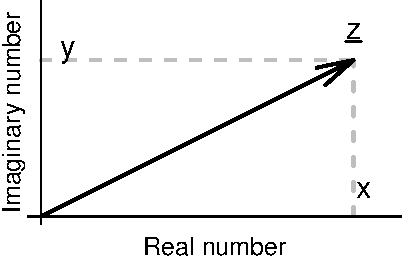
\includegraphics{Svetunkov---Svetunkov---Complex-Dynamic-Models_files/figure-latex/complexPlane-1.pdf}
\caption{\label{fig:complexPlane}Visual presentation of a complex number on the complex plane.}
\end{figure}

Any point lying on the complex plane in Figure \ref{fig:complexPlane} characterises a complex number, even if that point lies on the axis of real numbers. In that specific case, we would be talking about a complex number with a zero imaginary part, i.e.~\(\underline{z}=x+i0\).

Given that complex numbers can be represented on a plane (in so called Cartesian coordinates), the number \eqref{eq:complexNumber} can be represented in a form of a vector that starts in the origin of coordinates and ends at the point (x, y). Then any complex number can be represented in form of polar coordinates using the magnitude of the vector and its polar angle:
\begin{equation}
    \underline{z} = x+iy = r (\cos \phi + i \sin \phi),
    \label{eq:complexNumberTrigonometric}
\end{equation}
where \(r=|\underline{z}|\) is the magnitude, which is calculated as a Euclidean distance from the origin to the point (x, y) on the plane:
\begin{equation}
    r = \sqrt{x^2 + y^2},
    \label{eq:complexNumberMagnitude}
\end{equation}
and \(\phi=\Arg(\underline{z})\) is the angle, which equals to:
\begin{equation}
    \phi = \arctan \frac{y}{x} + 2 \pi l,
    \label{eq:complexNumberAngle}
\end{equation}
where \(l\) is an integer number. While depending on a task, \(l\) can be set to a positive, a negative number, or a zero, for convenience, we will restrict it to \(l=0\), because all the other values will not be useful for the inference in following chapters. The polar angle is sometimes referred to as the argument of a complex number.

Using the magnitude and the polar angle, we can also represent any complex number in the exponential form, which was first proposed in 1748 by Euler, in his book ``Introduction to the Infinitesimal Analysis'' \textbf{(Euler, 1961, pp.~118-119)}, which:
\begin{equation}
    \underline{z} = r e^{i \phi} ,
    \label{eq:complexNumberExponential}
\end{equation}
where \(e\) is the Euler's constant. Equation \eqref{eq:complexNumberExponential} is nowadays also called ``Euler's form''. Comparing @ref\{eq:complexNumberTrigonometric\} with @ref\{eq:complexNumberExponential\}, we can conclude that:
\begin{equation}
    e^{i \phi} = \cos \phi + i \sin \phi ,
    \label{eq:EulerFormula}
\end{equation}
which gives the connection between the linear, trigonometric and exponential forms of a complex number. In the exponential form \eqref{eq:complexNumberExponential}, a positive real number has \(\phi=0\), while a negative one has \(\phi=\pi\), and all imaginary numbers have an angle dividable by \(\frac{\pi}{2}\). So, for example:
\begin{equation*}
    \begin{aligned}
    41 = & 41 e^{i 0} \\
    i41 = & 41 e^{i \frac{\pi}{2}} \\
    -41 = & 41 e^{i \pi} \\
    -i41 = & 41 e^{i \frac{3 \pi}{2}}
    \end{aligned}
\end{equation*}
In fact, multiplication of any complex number by the imaginary unit implies the rotation of complex vector by \(\frac{\pi}{2}\), as shown in Figure \ref{fig:complexPlaneMultiplication}, where a complex number \(\underline{z}_1 = x_1 + i y_1\) becomes \(\underline{z}_2 = \underline{z}_1 \times i = x_2 + i y_2\) etc.

\begin{figure}
\centering
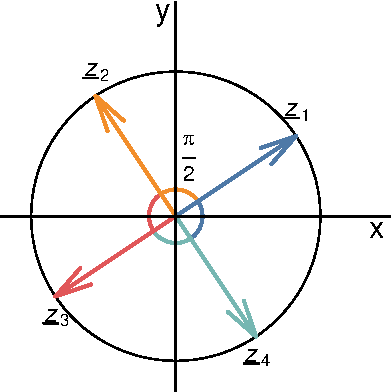
\includegraphics{Svetunkov---Svetunkov---Complex-Dynamic-Models_files/figure-latex/complexPlaneMultiplication-1.pdf}
\caption{\label{fig:complexPlaneMultiplication}Multiplication of a complex number by \(i\) implies the rotation of it by \(\frac{\pi}{2}\).}
\end{figure}

In a way, any mathematical operation with a complex number implies a change in magnitude and angle of the number, while the multiplication and division by a number with non-zero imaginary part will always lead to the rotation of the vector. Operations of addition and subtraction are simpler in the linear form:
\begin{equation*}
    \underline{z}_3 = \underline{z}_1 + \underline{z}_2 = x_1 + x_2 + i (y_1 + y_2) ,
\end{equation*}
while operations of multiplication and division are easier to do in either exponential or trigonometric forms of complex numbers:
\begin{equation*}
    \underline{z}_3 = \underline{z}_1 \times \underline{z}_2 = r_1 r_2 e^{i \phi_1 + \phi_2} 
\end{equation*}
or:
\begin{equation*}
    \underline{z}_3 = r_1 r_2 \left(\cos (\phi_1 + \phi_2) + i \sin (\phi_1 + \phi_2) \right) .
\end{equation*}

Furthermore, given that any complex number can be represented in the exponential form \eqref{eq:complexNumberExponential}, it can also be visualised on a polar coordinates plane, where the magnitude is marked on the x-axis, and the polar angle is marked on the y-axis. This is shown visually in Figure \ref{fig:complexPlanePolar}.

\begin{figure}
\centering
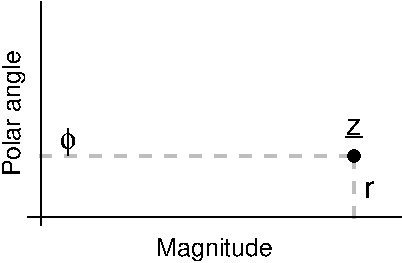
\includegraphics{Svetunkov---Svetunkov---Complex-Dynamic-Models_files/figure-latex/complexPlanePolar-1.pdf}
\caption{\label{fig:complexPlanePolar}Visual presentation of a complex number in the polar coordinates.}
\end{figure}

The usefulness of the polar coordinates presentation becomes apparent when a set of complex numbers is considered, because then in some cases it becomes possible to see some relations that are not obvious on the Cartesian plane. Figure \ref{fig:complexCartesianvsPolar} shows an example of a set of complex random numbers, for which the real and imaginary parts do not seem to have any obvious linear relation, but the magnitude and the angle have a negative relation.

\begin{figure}
\centering
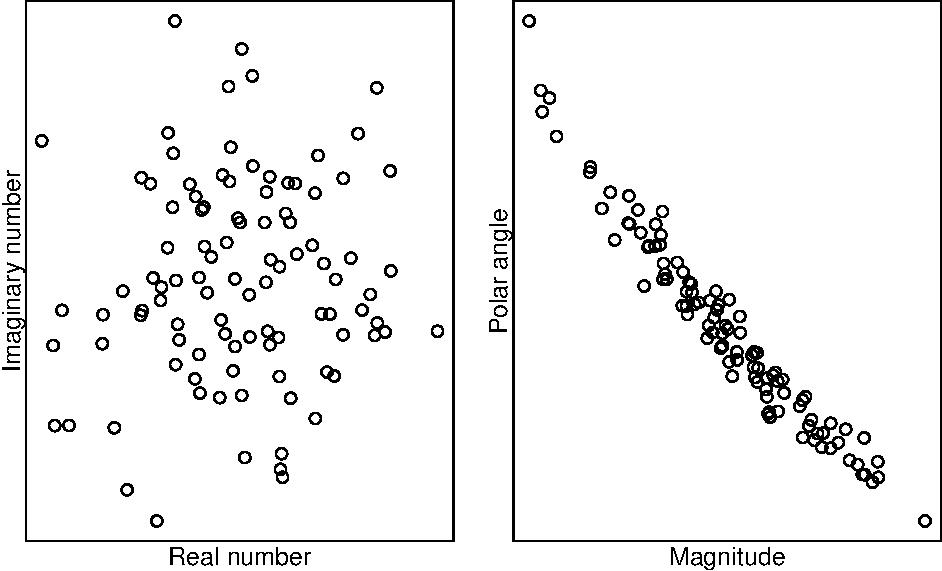
\includegraphics{Svetunkov---Svetunkov---Complex-Dynamic-Models_files/figure-latex/complexCartesianvsPolar-1.pdf}
\caption{\label{fig:complexCartesianvsPolar}Visualisation of a set of complex numbers on Cartesian and on polar coordinates planes.}
\end{figure}

In this case, modelling can be done in the exponential form of complex numbers, which might allow capturing complicated non-linear relations between variables.

When it comes to comparing complex numbers, mathematically we will say that two complex numbers \(\underline{z}_1 = x_1 + i y_1\) and \(\underline{z}_2 = x_2 + i y_2\) are equal to each other if and only if their real and imaginary parts are equal:
\begin{equation*}
    \underline{z}_1 = \underline{z}_2 \iff \left \lbrace
    \begin{aligned}
        & x_1 = x_2 \\
        & y_1 = y_2
    \end{aligned}
    \right. ,
\end{equation*}
which is equivalent to saying that their magnitudes and polar angles are equal:
\begin{equation*}
    \underline{z}_1 = \underline{z}_2 \iff \left \lbrace
    \begin{aligned}
        & |\underline{z}_1| = |\underline{z}_2| \\
        & \Arg(\underline{z}_1) = \Arg(\underline{z}_2)
    \end{aligned}
    \right. .
\end{equation*}

Unfortunately, given that complex numbers are two dimensional, it is not possible to say in general whether one number is greater or less than the other. However, we could use magnitude to compare complex numbers, to say which one lies further away from the origin than the other. In that case, the number with a larger magnitude could be considered as a greater than the one with the smaller magnitude. While we could compare the polar angles as well, they only give us information about rotation of a complex number and thus do not give any meaningful information about the comparison of numbers. So, two complex numbers in Figure \ref{fig:complexPlaneCircle} would have the same magnitude, but will have different angles, and it is not possible to say whether one number is greater than the other in this case. In order to conclude that, we would need to devise additional criteria for comparison of numbers (e.g.~positive numbers are ``better'' than the negative ones, thus \(\phi_1=\pi\) and \(\phi_1=-\pi\) is ``worse'' than \(\phi_2=0\)).

\begin{figure}
\centering
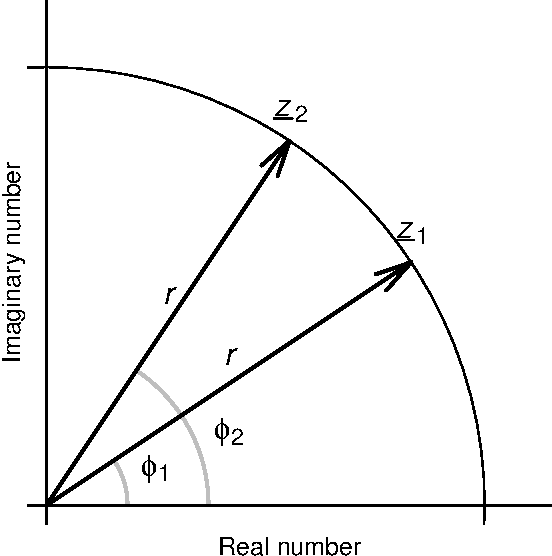
\includegraphics{Svetunkov---Svetunkov---Complex-Dynamic-Models_files/figure-latex/complexPlaneCircle-1.pdf}
\caption{\label{fig:complexPlaneCircle}Comparison of two complex numbers \(\underline{z}_1\) and \(\underline{z}_2\) that have the same magnitude \(r\), but different angles \(\phi_1\) and \(\phi_2\).}
\end{figure}

Continuing the discussion of different forms of a complex number, its magnitude can be represented in exponential form:
\begin{equation*}
    r = e^{\ln(r)},
\end{equation*}
where \(\ln\) is the natural logarithm. This can then be used to rewrite the exponential form of a complex number as:
\begin{equation}
    \underline{z} = e^{\ln r + i \phi} ,
    \label{eq:complexNumberExponentialAll}
\end{equation}
And this form allows calculating logarithms of a complex number:
\begin{equation*}
    \ln \underline{z} = \ln \left(e^{\ln r + i \phi} \right) = \ln r + i \phi .
\end{equation*}
This operation will become useful when we discuss transformations of complex-valued functions, but it also shows that a logarithm of a negative real number is a complex number, because in that case \(\phi=\pi\). This demonstrates that the field of complex numbers is complete: any mathematical operation of a complex number will give another complex number.

One of the important definitions in theory of complex numbers is the conjugate complex number. It is the number, for which the imaginary part has the sign opposite to the one of the original variable. For example, the conjugate of the complex variable \(\underline{z} = x+ iy\) is \(\underline{\tilde{z}} = x- iy\). These numbers are useful because the multiplication of a complex number by its conjugate gives a real number:
\begin{equation}
    \underline{z} \times \underline{\tilde{z}} = (x+ iy) (x- iy) = x^2 + y^2 ,
    \label{eq:complexNumberConjugateMulti}
\end{equation}
which is the square of the magnitude \eqref{eq:complexNumberMagnitude} of both complex variables \(\underline{z}\) and \(\underline{\tilde{z}}\). Conjugation is distributive over addition, subtraction, multiplication and division, meaning that:
\begin{equation}
    \begin{aligned}
        & \widetilde{x + y} = \tilde{x} + \tilde{y} \\
        & \widetilde{x - y} = \tilde{x} - \tilde{y} \\
        & \widetilde{x \times y} = \tilde{x} \times \tilde{y} \\
        & \widetilde{\left(\frac{x}{y}\right)} = \frac{\tilde{x}}{\tilde{y}} .
    \end{aligned}
    \label{eq:complexNumberConjugateDistributive}
\end{equation}

Finally, given that any complex number can be represented visually in a form of a vector, we can write it mathematically either like vector:
\begin{equation}
    \boldsymbol{z} = \begin{pmatrix} x \\ y \end{pmatrix}
    \label{eq:complexNumberVectors}
\end{equation}
or like a matrix:
\begin{equation}
    \underset{\sim}{\boldsymbol{z}} = \begin{pmatrix} x & -y \\ y & x \end{pmatrix} ,
    \label{eq:complexNumberMatrix}
\end{equation}
where the symbold \(\sim\) below the letter denotes a matrix presentation of a complex number. In the matrix notation, any real number can be represented as a diagonal matrix, while any imaginary one is a matrix with zero diagonal:
\begin{equation*}
    \begin{aligned}
        & \begin{pmatrix} x & 0 \\ 0 & x \end{pmatrix} \\
        & \begin{pmatrix} 0 & -y \\ y & 0 \end{pmatrix}
    \end{aligned} .
\end{equation*}
All the mathematical operations done with the vector and matrix representations would correspond to the ones for the conventional complex numbers. Furthermore, the multiplication by the transpose of the original object in both of these cases is equivalent to the multiplication by the conjugate value \eqref{eq:complexNumberConjugateMulti}. For the vector:
\begin{equation}
    \boldsymbol{z} \boldsymbol{z}^\prime \begin{pmatrix} x & y \end{pmatrix} \times \begin{pmatrix} x \\ y \end{pmatrix} = \begin{pmatrix} x^2 + y^2 \end{pmatrix}
    \label{eq:complexNumberVectorsMulti}
\end{equation}
and for the matrix:
\begin{equation}
    \underset{\sim}{\boldsymbol{z}} \underset{\sim}{\boldsymbol{z}}^\prime = \begin{pmatrix} x & -y \\ y & x \end{pmatrix} \times \begin{pmatrix} x & y \\ -y & x \end{pmatrix} = 
    \begin{pmatrix} x^2 + y^2 & 0 \\ 0 & x^2 + y^2 \end{pmatrix}.
    \label{eq:complexNumberMatrixMulti}
\end{equation}
These transpositions will be called in this monograph ``conjugate transpositions''. The vector and matrix representations become especially useful when we work with complex variables to construct complex models. Finally, in case of matrix form, it is possible to multiply complex variable by itself without the conjugation, which results in:
\begin{equation}
    \underset{\sim}{\boldsymbol{z}} \underset{\sim}{\boldsymbol{z}}^{\top} = \begin{pmatrix} x & -y \\ y & x \end{pmatrix} \times \begin{pmatrix} x & -y \\ y & x \end{pmatrix} = 
    \begin{pmatrix} x^2 - y^2 & - 2 xy \\ 2 xy & x^2 - y^2 \end{pmatrix}.
    \label{eq:complexNumberMatrixMultiDirect}
\end{equation}
In this monograph, we will call the multiplications \eqref{eq:complexNumberMatrixMulti} and \eqref{eq:complexNumberMatrixMultiDirect} ``conjugate'' and ``direct'' respectively.

\hypertarget{complexVariable}{%
\subsection{Complex variables}\label{complexVariable}}

Similarly to any other variable, complex variable is a place holder for values, with the difference that it represents two parts of a number instead of one. Given the properties of complex numbers discussed in the previous section, any complex variable can be represented in linear, trigonometric and exponential forms. But in addition, it can also be represented in the form of a set of equations, i.e.~if \(y_r + i y_i = 3+2i\) then:
\begin{equation}
    \begin{aligned}
        y_r = & 3 \\
        y_i = & 2
    \end{aligned} ,
    \label{eq:complexVariablesSystem}
\end{equation}
where the subscript \(r\) or \(i\) refers to respectively the real or imaginary parts of the complex number. In fact, any function of a complex variable can be represented as system of two equations, so that for a function
\begin{equation}
    y_{r} + i y_{i} = f(x_r+ix_i)
    \label{eq:complexFunction}
\end{equation}
we have:
\begin{equation}
    \begin{aligned}
        y_r = & \mathcal{R}(f(x_r+ix_i)) \\
        y_i = & \mathcal{I}(f(x_r+ix_i))
    \end{aligned} ,
    \label{eq:complexFunctionSystem}
\end{equation}
where \(\mathcal{R}()\) and \(\mathcal{I}()\) are respectively the real and the imaginary parts of a resulting complex variable. For example, a simple linear function:
\begin{equation*}
    y_r + i y_i = a_{0,r} + i a_{0,i} + (a_{1,r} + i a_{1,i}) (x_{1,r} + i x_{1,i}),
\end{equation*}
which can be written after opening the brackets and regrouping elements as:
\begin{equation*}
    y_r + i y_i = a_{0,r} + a_{1,r} x_{1,r} - a_{1,i} x_{1,i} + i \left( a_{0,i} + a_{1,i} x_{1,r} + a_{1,r} x_{1,i} \right)
\end{equation*}
and is equivalent to the system of the following two equations:
\begin{equation*}
    \begin{aligned}
        y_r = & a_{0,r} + a_{1,r} x_{1,r} - a_{1,i} x_{1,i} \\
        y_i = & a_{0,i} + a_{1,i} x_{1,r} + a_{1,r} x_{1,i}
    \end{aligned} .
\end{equation*}
Given the vector and matrix representation of complex variables, the same linear function can be written as:
\begin{equation*}
    \begin{pmatrix} y_r \\ y_i \end{pmatrix} = \begin{pmatrix} a_{0,r} \\ a_{0,i} \end{pmatrix} + \begin{pmatrix} a_{1,r} & -a_{1,i} \\ a_{1,i} & a_{1,r} \end{pmatrix} \begin{pmatrix} x_{1,r} \\ x_{1,i} \end{pmatrix} ,
\end{equation*}
which is convenient in some situations. Presenting the system of equations \eqref{eq:complexFunctionSystem} in the linear form \eqref{eq:complexFunction} is often convenient. In fact, any function of complex variables can be represented as a system of two functions. Even if the real or the imaginary part of the output complex variable \(y_r + i y_i\) is equal to zero, we can still use a system of two equations, where one of the equations becomes just a constraint for the function. For example, if we assume that \(y_i=0\), then the system \eqref{eq:complexFunctionSystem} becomes:
\begin{equation*}
    \begin{aligned}
        & y_r = \mathcal{R}(f(x_r+ix_i)) \\
        & \mathcal{I}(f(x_r+ix_i)) = 0
    \end{aligned} .
\end{equation*}
This property becomes especially useful if one needs to construct a model with linear relations between the input variables \citep[this is discussed in Chapter ??? of][]{Svetunkov2014}.

Given the discussion about the vector and matrix forms of complex numbers, the system of equations \eqref{eq:complexFunctionSystem} can be written as:
\begin{equation}
    \begin{pmatrix} y_r \\ y_i \end{pmatrix} =
    \begin{pmatrix} \mathcal{R}(f(x_r+ix_i)) \\ \mathcal{I}(f(x_r+ix_i)) \end{pmatrix} .
    \label{eq:complexFunctionVectors}
\end{equation}
or:
\begin{equation}
    \begin{pmatrix} \mathcal{R}(f(x_r+ix_i)) & - \mathcal{I}(f(x_r+ix_i)) \\ \mathcal{I}(f(x_r+ix_i)) & \mathcal{R}(f(x_r+ix_i)) \end{pmatrix} .
    \label{eq:complexFunctionMatrix}
\end{equation}
The representations \eqref{eq:complexFunction}, \eqref{eq:complexFunctionSystem}, \eqref{eq:complexFunctionVectors} and \eqref{eq:complexFunctionMatrix} are equivalent and can be used interchangeably depending on the task at hand.

Finally, in terms of definitions, the function \eqref{eq:complexFunction} is often referred to as a ``complex-valued'' function. It maps a certain values of the input variable \(x_r + i x_i\) with a specific value of the output variable \(y_r +i y_i\). If there is only a one-to-one relation between the input and output variables then such function is called ``univalent''. When several different values of the input variable leads to one and the same value of the output variable then the function is called ``multivalent''. An example of the former is the linear function:
\begin{equation*}
    y_r + i y_i = (a_{1,r} + i a_{1,i}) (x_{1,r} + i x_{1,i}),
\end{equation*}
while for the latter, an example is
\begin{equation*}
    y_r + i y_i = (a_{1,r} + i a_{1,i}) (x_{1,r} + i x_{1,i})^2, 
\end{equation*}
where two different input complex numbers (for example \(0 + i\) and \(0-i\)) correspond to the same output number (\(-1 + i0\)). While there are examples of functions like that in the real domain, in the complex one, they appear even more often due to the rotation property discussed in the previous Subsection.

\hypertarget{vectorComplexVariables}{%
\subsection{Vectors of complex variables}\label{vectorComplexVariables}}

Last but not least, for what follows, we introduce vectors and matrices of complex variables. There are different ways how one can represent a vector of complex variables. The simplest and most direct one is:
\begin{equation}
    \underline{\mathbf{x}} = \begin{pmatrix} x_{r,1} + i x_{i,1} \\ x_{r,2} + i x_{i,2} \\ x_{r,3} + i x_{i,3} \end{pmatrix} ,
    \label{eq:complexVector}
\end{equation}
where the index in subscript (1, 2, 3) represents the observed first, second and third values of the complex variable. Alternatively, given that any complex variable can be represented as a vector \eqref{eq:complexNumberVectors}, the same complex vector can be written as a matrix:
\begin{equation}
    \mathbf{x} = \begin{pmatrix} x_{r,1} & x_{i,1} \\ x_{r,2} & x_{i,2} \\ x_{r,3} & x_{i,3} \end{pmatrix} ,
    \label{eq:complexVectorMatrix}
\end{equation}
Finally, given the connection of complex numbers and matrices \eqref{eq:complexNumberMatrix}, the same complex vector \(x\) can be written as a matrix:
\begin{equation}
    \underset{\sim}{\mathbf{x}} = \begin{pmatrix} x_{r,1} & - x_{i,1} \\ x_{i,1} & x_{r,1} \\
                                 x_{r,2} & - x_{i,2} \\ x_{i,2} & x_{r,2} \\
                                 x_{r,3} & - x_{i,3} \\ x_{i,3} & x_{r,3} \end{pmatrix} .
    \label{eq:complexMatrix}
\end{equation}
We use the symbol \(\sim\) below a character to denote the complex variable in the matrix form \eqref{eq:complexMatrix}. Each of the forms \eqref{eq:complexVector}, \eqref{eq:complexVectorMatrix} and \eqref{eq:complexMatrix} might be useful in different circumstances, their usage should be dictated by the modelling purpose.

Finally, note that the transposition of these three forms will imply different things. As discussed earlier, in vector and matrix forms transposition of a complex number implies the conjugation. However, transposing \eqref{eq:complexVector} will not have the same effect - it will only switch rows and columns of the complex vector:
\begin{equation}
    \underline{\mathbf{x}}^{\top} = \begin{pmatrix} x_{r,1} + i x_{i,1} & x_{r,2} + i x_{i,2} & x_{r,3} + i x_{i,3}
                        \end{pmatrix} ,
    \label{eq:complexVectorTransposed}
\end{equation}
If we then switch to either the form \eqref{eq:complexNumberVectors} or \eqref{eq:complexNumberMatrix}, we will not get the vector of conjugate complex numbers, but rather an object of the original complex variables with the switched rows and columns:
\begin{equation}
    {\mathbf{x}}^{\top} = \begin{pmatrix} x_{r,1} & x_{r,2} & x_{r,3} \\
                                 x_{i,1} & x_{i,2} & x_{i,3}
                        \end{pmatrix} 
    \label{eq:complexVectorMatrixTransposed}
\end{equation}
and
\begin{equation}
    \underset{\sim}{\mathbf{x}}^{\top} = \begin{pmatrix} x_{r,1} & - x_{i,1} & x_{r,2} & - x_{i,2} & x_{r,3} & - x_{i,3} \\
                                        x_{i,1} & x_{r,1} & x_{i,2} & x_{r,2} & x_{i,3} & x_{r,3}
                        \end{pmatrix} .
    \label{eq:complexMatrixTransposed}
\end{equation}
We will denote the operation of transposition above with the symbol \(\top\) and will call it just ``transposition''. The transposition that produces the conjugate complex numbers is called ``conjugate transposition'' and will be denoted as \(\prime\) in this monograph. For the three examples above, the conjugate transposition will be:
\begin{equation}
    \underline{\mathbf{x}}^{\prime} = \begin{pmatrix} x_{r,1} - i x_{i,1} & x_{r,2} - i x_{i,2} & x_{r,3} - i x_{i,3}
                        \end{pmatrix} ,
    \label{eq:complexVectorTransposedConj}
\end{equation}
\begin{equation}
    {\mathbf{x}}^{\prime} = \begin{pmatrix} x_{r,1} & x_{r,2} & x_{r,3} \\
                                         -x_{i,1} & -x_{i,2} & -x_{i,3}
                        \end{pmatrix} 
    \label{eq:complexVectorMatrixTransposedConj}
\end{equation}
and
\begin{equation}
    \underset{\sim}{\mathbf{x}}^{\prime} = \begin{pmatrix} x_{r,1} & x_{i,1} & x_{r,2} & x_{i,2} & x_{r,3} & x_{i,3} \\
                                        -x_{i,1} & x_{r,1} & -x_{i,2} & x_{r,2} & -x_{i,3} & x_{r,3}
                        \end{pmatrix} .
    \label{eq:complexMatrixTransposedConj}
\end{equation}

\hypertarget{complexRandomVariable}{%
\section{Complex random variable}\label{complexRandomVariable}}

In statistics, a random variable is a variable, the value of which depends on random events. For example, for the classical coin tossing experiment, \(x\) would be considered as a random variable if it is equal to 1 in case of heads and is equal to zero otherwise. In case of complex random variables (c.r.v.), the logic is similar, but we would typically deal with two-dimensional cases (e.g.~tossing two coins simultaneously). We accept that in some cases, some parts of the c.r.v. might become non-random (e.g.~the real part becomes equal to some fixed number). As such, we would be saying that \(x=x_r+ix_i\) is a complex random variable if at least one part of it follows some distribution. Furthermore, while random variables can be measured in a variety of scales (coin tossing represents the nominal scale), in this monograph we focus the discussion on continuous numerical variables.

As any other random variable, c.r.v. can be characterised by its moments. However, some of its moments differ from the conventional ones for real variables and are based on the properties of complex numbers.

\hypertarget{first-moment}{%
\subsection{First moment}\label{first-moment}}

The first moment of any c.r.v. is relatively straightforward. For the variable \(\underline{x}=x_r+ix_i\) it is:
\begin{equation}
    \underline{\mu} = \mathrm{E}(\underline{x}) = \mathrm{E}(x_r + i x_i) = \mathrm{E}(x_r) + i \mathrm{E}(x_i) = \mu_{r} + i \mu_{i},
    \label{eq:crvMomentFirst}
\end{equation}
due to the law of total expectation and because \(i\) is a constant. In \eqref{eq:crvMomentFirst}, \(\mathrm{E}(.)\) is the expectation of a variable, \(\underline{\mu}\) is the first moment of a complex variable and \(\mu_{r}\) and \(\mu_{i}\) are the respective real and imaginary parts of the first moment. In sample, this moment can be calculated as:
\begin{equation}
    \underline{\hat{\mu}} = \hat{\mu}_{r} + i \hat{\mu}_{i} = \frac{1}{n}\sum_{j=1}^n x_{r,j} + i \frac{1}{n}\sum_{j=1}^n x_{i,j},
    \label{eq:crvMomentFirstSample}
\end{equation}
where \(n\) is the sample size and \(\hat{\mu}\) is the estimate of \(\mu\). The properties of the first moment of c.r.v. are similar to the properties of any other random variable. The only thing to note is that the moment can also be represented in a vector or matrix form (see Subsection \ref{complexVariable}):
\begin{equation}
    \boldsymbol{\mu} = \begin{pmatrix} \mu_{r} \\ \mu_{i} \end{pmatrix} 
    \label{eq:crvMomentsVector}
\end{equation}
or
\begin{equation}
    \underset{\sim}{\boldsymbol{\mu}} = \begin{pmatrix} \mu_{r} & - \mu_{i} \\ \mu_{i} & \mu_{r} \end{pmatrix} .
    \label{eq:crvMomentsMatrix}
\end{equation}

In R, the first moment can be obtained via the \texttt{mean()} function from \texttt{stats} package:

\begin{Shaded}
\begin{Highlighting}[]
\CommentTok{\# Create a random variable}
\NormalTok{x }\OtherTok{\textless{}{-}} \FunctionTok{complex}\NormalTok{(}\AttributeTok{real=}\FunctionTok{rnorm}\NormalTok{(}\DecValTok{100}\NormalTok{, }\AttributeTok{mean=}\DecValTok{50}\NormalTok{, }\AttributeTok{sd=}\DecValTok{10}\NormalTok{),}
             \AttributeTok{imaginary=}\FunctionTok{rnorm}\NormalTok{(}\DecValTok{100}\NormalTok{, }\AttributeTok{mean=}\DecValTok{100}\NormalTok{, }\AttributeTok{sd=}\DecValTok{10}\NormalTok{))}
\CommentTok{\# Calculate the first moment}
\FunctionTok{mean}\NormalTok{(x)}
\end{Highlighting}
\end{Shaded}

\begin{verbatim}
## [1] 49.5654+100.385i
\end{verbatim}

\hypertarget{crvSecondMoment}{%
\subsection{Second moment}\label{crvSecondMoment}}

While there are raw moments for c.r.v., here we will focus on the centred ones, i.e.~moments for \(x-\bar{x}\). There are several instruments related to the second moment that could characterise a complex random variable. The first one is called ``variance'' and is based on the multiplication by a conjugate number \citep{reference}. So for the c.r.v. \(x_r + i x_i\) the variance is:
\begin{equation}
    \begin{aligned}
    \sigma_x^2 = & \mathrm{E}((x-\mu) (\tilde{x}-\tilde{\mu})) = \\
                 & \mathrm{E}\left(((x_r-\mu_{r}) + i (x_i-\mu_{i}))((x_r-\mu_{r}) - i (x_i-\mu_{i}))\right) = \\
                 & \mathrm{E}((x_r-\mu_{r})^2) +  \mathrm{E}((x_i-\mu_{i})^2)
    \end{aligned}
    \label{eq:crvMomentSecondVariance}
\end{equation}
or taking that the variances of the real and the imaginary parts are \(\sigma_{x_r}^2\) and \(\sigma_{x_i}^2\) respectively:
\begin{equation}
    \sigma_x^2 = \sigma_{x_r}^2 + \sigma_{x_i}^2.
    \label{eq:crvMomentSecondVarianceShort}
\end{equation}
Multiplication by conjugate in \eqref{eq:crvMomentSecondVariance} allows keeping the size of variability for both real and imaginary parts, but at the same time masks the individual contribution of each part in the overall variance and removes the covariance between the parts. The resulting values shows in a way the overall variability of a c.r.v. along a diagonal line as shown in Figure \ref{fig:crvMomentSecondVariance}.

\begin{figure}
\centering
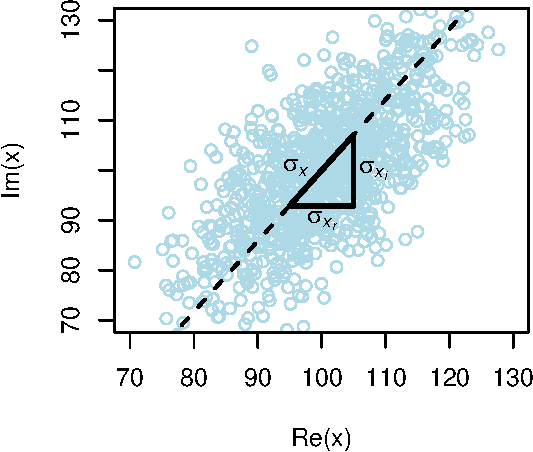
\includegraphics{Svetunkov---Svetunkov---Complex-Dynamic-Models_files/figure-latex/crvMomentSecondVariance-1.pdf}
\caption{\label{fig:crvMomentSecondVariance}Visual representation of variance of a complex random variable.}
\end{figure}

Figure \ref{fig:crvMomentSecondVariance} demonstrates graphically the relation between standard deviations of real, imaginary and the overall variance of a complex variable according to the formula \eqref{eq:crvMomentSecondVarianceShort}.

\citet{Picinbono} note that the moment \eqref{eq:crvMomentSecondVarianceShort} is not sufficient to entirely describe the second order statistics of a c.r.v. This is because it ignores the potential covariance between the parts of a variable and only describes their average variability. Another measure of variability of a complex random variable is the so called ``pseudo-variance'' \citep{reference}, which can be obtained by applying the conventional formula of variance directly to the c.r.v. without the multiplication by conjugate:
\begin{equation}
    \begin{aligned}
    \varsigma_x^2 = & \mathrm{E}(x-\mu^2) = \mathrm{E}\left(((x_r-\mu_{r}) + i (x_i-\mu_{i}))^2\right) = \\
                    & \mathrm{E}((x_r-\mu_{r})^2) - \mathrm{E}((x_i-\mu_{i})^2) + i2 \mathrm{E}((x_r-\mu_{r})(x_i-\mu_{i}))
    \end{aligned}
    \label{eq:crvMomentSecondVariancePseudo}
\end{equation}
or using the notation \(\sigma_{x_r,x_i}\) for covariance between the real and imaginary parts:
\begin{equation}
    \varsigma_x^2 = \sigma_{x_r}^2 - \sigma_{x_i}^2 + i2 \sigma_{x_r,x_i}.
    \label{eq:crvMomentSecondVariancePseudoShort}
\end{equation}
In the literature, the moment \eqref{eq:crvMomentSecondVariancePseudoShort} is called pseudo-variance \citep{reference}, because it does not measure the variability of a variable, but rather gives a different information: it shows whether the real and imaginary variances are similar and what the covariance between them is. If both real and imaginary parts of \eqref{eq:crvMomentSecondVariancePseudoShort} are equal to zero then it is said that the distribution of the complex variable \(x\) is spherical \citep{reference}, i.e.~the variances are similar and the real and imaginary parts are not linearly related. Furthermore, we should point out that while minimising \eqref{eq:crvMomentSecondVarianceShort} implies minimising both variances of the real and imaginary parts of \(x\) (ignoring the covariance between them), minimising \eqref{eq:crvMomentSecondVariancePseudoShort} is not as straightforward. At very least, we could tell that it implies making the distribution of \(x\) closer to the spherical one, but we cannot provide any thorough insight about this.

We should note that both measures can be considered as complex, and the main distinction between them is the multiplication by the same c.r.v or by its conjugate. As such we propose to call them respectively ``conjugate variance'' and ``direct variance''.

In R, the conjugate and direct variances are available in \texttt{cvar()} function of \texttt{complex} package.

\begin{Shaded}
\begin{Highlighting}[]
\CommentTok{\# Create a random variable}
\NormalTok{x }\OtherTok{\textless{}{-}} \FunctionTok{complex}\NormalTok{(}\AttributeTok{real=}\FunctionTok{rnorm}\NormalTok{(}\DecValTok{100}\NormalTok{, }\AttributeTok{mean=}\DecValTok{50}\NormalTok{, }\AttributeTok{sd=}\DecValTok{5}\NormalTok{),}
             \AttributeTok{imaginary=}\FunctionTok{rnorm}\NormalTok{(}\DecValTok{100}\NormalTok{, }\AttributeTok{mean=}\DecValTok{100}\NormalTok{, }\AttributeTok{sd=}\DecValTok{10}\NormalTok{))}
\CommentTok{\# Calculate the conjugate variance}
\FunctionTok{cvar}\NormalTok{(x, }\AttributeTok{method=}\StringTok{"conjugate"}\NormalTok{) }\SpecialCharTok{|\textgreater{}}
    \FunctionTok{setNames}\NormalTok{(}\StringTok{"Conjugate variance"}\NormalTok{)}
\end{Highlighting}
\end{Shaded}

\begin{verbatim}
## Conjugate variance 
## 150.509+0i
\end{verbatim}

\begin{Shaded}
\begin{Highlighting}[]
\CommentTok{\# Calculate the direct variance}
\FunctionTok{cvar}\NormalTok{(x, }\AttributeTok{method=}\StringTok{"direct"}\NormalTok{) }\SpecialCharTok{|\textgreater{}}
    \FunctionTok{setNames}\NormalTok{(}\StringTok{"Direct variance"}\NormalTok{)}
\end{Highlighting}
\end{Shaded}

\begin{verbatim}
##    Direct variance 
## -96.64872-1.23656i
\end{verbatim}

As we see from the output above, the direct variance has the negative real part, which indicates that the imaginary part has higher variance than the real one. The imaginary part of the direct variance shows the double covariance between the real and imaginary parts. Finally, the conjugate variance should be \(5^2 + 10^2 = 125\), but due to small sample (100 observations in the generated random variable above), it will be equal to a number close to it.

Given that any complex variable can be represented in a vector form, the c.r.v. \(x\) can be treated as a bivariate random variable, for which a covariance matrix can be calculated via:
\begin{equation}
    \boldsymbol{\Sigma}_x = \begin{pmatrix} \sigma_{x_r}^2 & \sigma_{x_r, x_i} \\ \sigma_{x_r, x_i} & \sigma_{x_i}^2 \end{pmatrix} .
    \label{eq:crvMomentSecondVarianceMatrix}
\end{equation}
The minimisation of the matrix \eqref{eq:crvMomentSecondVarianceMatrix} does not make sense, but instead it is possible to minimise the determinant of that matrix, which is called ``Generalised Variance'' (GV):
\begin{equation}
    \mathrm{GV} = |\boldsymbol{\Sigma}_x| = \sigma_{x_r}^2 \sigma_{x_i}^2 - \sigma_{x_r, x_i}^2 .
    \label{eq:crvMomentSecondGV}
\end{equation}

In R, this is implemented in \texttt{covar()} function from the \texttt{complex} package:

\begin{Shaded}
\begin{Highlighting}[]
\FunctionTok{covar}\NormalTok{(x)}
\end{Highlighting}
\end{Shaded}

\begin{verbatim}
##            x_r         x_i
## x_r 26.9301538  -0.6182819
## x_i -0.6182819 123.5788712
\end{verbatim}

The minimisation of GV, as can be seen from the formula \eqref{eq:crvMomentSecondGV}, implies the simultaneous minimisation of variances of real and imaginary parts and maximisation of the square of covariance between them, making the resulting distribution compacter and emphasising the potential relations between the real and imaginary parts of a c.r.v. For our example in R, the GV equals to:

\begin{Shaded}
\begin{Highlighting}[]
\FunctionTok{covar}\NormalTok{(x) }\SpecialCharTok{|\textgreater{}} \FunctionTok{det}\NormalTok{()}
\end{Highlighting}
\end{Shaded}

\begin{verbatim}
## [1] 3327.616
\end{verbatim}

All the three moments discussed in this subsection rely on variances of real and imaginary parts of a c.r.v. and on a covariance between those parts. These moments in turn can be calculated using the conventional formulae, correcting for the potential small sample bias \citep{referenceSBA}:
\begin{equation}
    \begin{aligned}
        \hat{\sigma}_{x_r}^2 = & \frac{1}{n-k} \sum_{j=1}^n (x_{r,j}-\bar{x}_{r,j})^2 \\
        \hat{\sigma}_{x_i}^2 = & \frac{1}{n-k} \sum_{j=1}^n (x_{i,j}-\bar{x}_{i,j})^2 \\
        \hat{\sigma}_{x_r, x_i} = & \frac{1}{n-k} \sum_{j=1}^n (x_{r,j}-\bar{x}_{r,j})(x_{i,j}-\bar{x}_{i,j})^2 ,
    \end{aligned}
    \label{eq:crvMomentSecondSample}
\end{equation}
where \(k\) is the number of estimated parameters in a model.

Finally, similar to the variance it is possible to calculate second moments between two complex random variables \(x = x_r+i x_i\) and \(y = y_r + i y_i\) \citep{Picinbono}. The ``conjugate'' covariance is calculated similarly to \eqref{eq:crvMomentSecondVariance} via the multiplication by conjugate:
\begin{equation}
    \begin{aligned}
    \sigma_{x,y} = & \mathrm{E}((\tilde{x}-\tilde{\mu}_x) (y-\mu_y)) = \\
                   & \mathrm{E}\left(((x_r-\mu_{x,r}) - i (x_i-\mu_{x,i}))((y_r-\mu_{y,r}) + i (y_i-\mu_{y,i}))\right) = \\
                   & \mathrm{E}((x_r-\mu_{x,r})(y_r-\mu_{y,r})) + \mathrm{E}((x_i-\mu_{x,i})(y_i-\mu_{y,i})) + \\
                   & i \left(\mathrm{E}((x_r-\mu_{x,r})(y_i-\mu_{y,i})) - \mathrm{E}((x_i-\mu_{x,i})(y_r-\mu_{y,r}))\right)
    \end{aligned}
    \label{eq:crvMomentSecondCovariance}
\end{equation}
where \(\mu_{x}\) and \(\mu_y\) are the respective first moments of c.r.v. \(x\) and \(y\). Using the notations above, the same covariance can be rewritten as:
\begin{equation}
    \sigma_{x,y} = \sigma_{x_r, y_r} + \sigma_{x_i, y_i} + i (\sigma_{x_r, y_i} - \sigma_{x_i, y_r}),
    \label{eq:crvMomentSecondCovarianceShort}
\end{equation}
which similarly to the variance \eqref{eq:crvMomentSecondVarianceShort} mixes the moments of the real and imaginary parts of the two random variables. Note though that if the conjugate of \(y\) is used instead of the conjugate of \(x\), the imaginary part of the covariance \eqref{eq:crvMomentSecondCovarianceShort} will change to \(\sigma_{x_i, y_r} - \sigma_{x_r, y_i}\), giving potentially different information about the relation between the variables.

In order to have more information about a c.r.v., we also need to consider the ``direct'' covariance \citep[also known in the literature as pseudo-covariance,][]{reference}, which can be shown to be equal to:
\begin{equation}
    \varsigma_{x,y} = \sigma_{x_r, y_r} - \sigma_{x_i, y_i} + i (\sigma_{x_i, y_r} + \sigma_{x_r, y_i}).
    \label{eq:crvMomentSecondPseudoCovarianceShort}
\end{equation}
Note that none of these moments on its own gives enough information about the relation between two complex variables, so they need to be used jointly. Alternatively, using vector representation, a covariance matrix between the two c.r.v. can be used to get a better understanding about the relations between them:
\begin{equation}
    \boldsymbol{\Sigma}_{x,y} =
        \begin{pmatrix}
            \sigma_{x_r}^2 & \sigma_{x_r, x_i} & \sigma_{x_r, y_r} & \sigma_{x_r, y_i} \\
            \sigma_{x_r, x_i} & \sigma_{x_i}^2 & \sigma_{x_i, y_r} & \sigma_{x_i, y_i} \\
            \sigma_{x_r, y_r} & \sigma_{x_i, y_r} & \sigma_{y_r}^2 & \sigma_{y_r, y_i} \\
            \sigma_{x_r, y_i} & \sigma_{x_i, y_i} & \sigma_{y_r, y_i} & \sigma_{y_i}^2
        \end{pmatrix} .
    \label{eq:crvMomentSecondCoVarianceMatrix}
\end{equation}

In R, the complex covariances are implemented in \texttt{ccov()} function from the \texttt{complex} package:

\begin{Shaded}
\begin{Highlighting}[]
\CommentTok{\# Create a random variable x}
\NormalTok{x }\OtherTok{\textless{}{-}} \FunctionTok{complex}\NormalTok{(}\AttributeTok{real=}\FunctionTok{rnorm}\NormalTok{(}\DecValTok{100}\NormalTok{, }\AttributeTok{mean=}\DecValTok{50}\NormalTok{, }\AttributeTok{sd=}\DecValTok{5}\NormalTok{),}
             \AttributeTok{imaginary=}\FunctionTok{rnorm}\NormalTok{(}\DecValTok{100}\NormalTok{, }\AttributeTok{mean=}\DecValTok{100}\NormalTok{, }\AttributeTok{sd=}\DecValTok{10}\NormalTok{))}
\CommentTok{\# Create a random variable y}
\NormalTok{y }\OtherTok{\textless{}{-}}\NormalTok{ (}\FloatTok{1.5} \SpecialCharTok{+}\NormalTok{ 3i) }\SpecialCharTok{+}\NormalTok{ (}\FloatTok{0.5} \SpecialCharTok{{-}} \FloatTok{0.75}\NormalTok{i) }\SpecialCharTok{*}\NormalTok{ x }\SpecialCharTok{+}
            \FunctionTok{complex}\NormalTok{(}\AttributeTok{real=}\FunctionTok{rnorm}\NormalTok{(}\DecValTok{100}\NormalTok{, }\AttributeTok{mean=}\DecValTok{0}\NormalTok{, }\AttributeTok{sd=}\DecValTok{10}\NormalTok{),}
                    \AttributeTok{imaginary=}\FunctionTok{rnorm}\NormalTok{(}\DecValTok{100}\NormalTok{, }\AttributeTok{mean=}\DecValTok{0}\NormalTok{, }\AttributeTok{sd=}\DecValTok{10}\NormalTok{))}
\CommentTok{\# Calculate the conjugate variance}
\FunctionTok{ccov}\NormalTok{(x, y, }\AttributeTok{method=}\StringTok{"conjugate"}\NormalTok{) }\SpecialCharTok{|\textgreater{}}
    \FunctionTok{setNames}\NormalTok{(}\StringTok{"Conjugate covariance"}\NormalTok{)}
\end{Highlighting}
\end{Shaded}

\begin{verbatim}
## Conjugate covariance 
## 52.5628-94.99459i
\end{verbatim}

\begin{Shaded}
\begin{Highlighting}[]
\CommentTok{\# Calculate the direct variance}
\FunctionTok{ccov}\NormalTok{(x, y, }\AttributeTok{method=}\StringTok{"direct"}\NormalTok{) }\SpecialCharTok{|\textgreater{}}
    \FunctionTok{setNames}\NormalTok{(}\StringTok{"Direct covariance"}\NormalTok{)}
\end{Highlighting}
\end{Shaded}

\begin{verbatim}
##   Direct covariance 
## -39.23729+44.04638i
\end{verbatim}

The functions \texttt{cvar()} and \texttt{ccov()} also accept a matrix instead of vector \texttt{x}, in which case they will produce a matrix of moments with complex variances on diagonal and complex covariances on the off-diagonals.

\begin{Shaded}
\begin{Highlighting}[]
\NormalTok{ourData }\OtherTok{\textless{}{-}} \FunctionTok{cbind}\NormalTok{(x,y)}
\FunctionTok{cvar}\NormalTok{(ourData, }\AttributeTok{method=}\StringTok{"direct"}\NormalTok{)}
\end{Highlighting}
\end{Shaded}

\begin{verbatim}
##                     x                   y
## x -68.23133-13.61148i -39.23729+44.04638i
## y -39.23729+44.04638i   6.43149+57.71384i
\end{verbatim}

While there exist higher order moments for complex random variables, we do not discuss them in this book.

\hypertarget{parametric-distributions-of-c.r.v.}{%
\section{Parametric Distributions of c.r.v.}\label{parametric-distributions-of-c.r.v.}}

Similarly to the real valued random variables, complex random variables can follow some parametric distributions. In this section, we discuss several simple ones, some of which will be used later in this monograph.

In general, it is reasonable to assume that a c.r.v. has a distribution of a shape of a circle or ellipse on the complex plane. This becomes more apparent if we consider the exponential form of a c.r.v. \eqref{eq:complexNumberExponential} and consider both magnitude and the angle as random variables. In the simplest case, when they are not correlated and we consider a variable that is centred around the origin, the randomness coming from both of these components will result in a circle on the complex plane, see the following example in R (and Figure \ref{fig:crvGeneratedCircle}):

\begin{Shaded}
\begin{Highlighting}[]
\CommentTok{\# Generate magnitudes from the uniform distribution}
\NormalTok{R }\OtherTok{\textless{}{-}} \FunctionTok{runif}\NormalTok{(}\DecValTok{1000}\NormalTok{,}\DecValTok{0}\NormalTok{,}\DecValTok{10}\NormalTok{)}
\CommentTok{\# Generate angles from the uniform distribution}
\NormalTok{phi }\OtherTok{\textless{}{-}} \FunctionTok{runif}\NormalTok{(}\DecValTok{1000}\NormalTok{,}\SpecialCharTok{{-}}\NormalTok{pi,pi)}
\CommentTok{\# Create c.r.v in exponential form}
\NormalTok{x }\OtherTok{\textless{}{-}}\NormalTok{ R }\SpecialCharTok{*} \FunctionTok{exp}\NormalTok{(}\FunctionTok{complex}\NormalTok{(}\AttributeTok{imaginary=}\NormalTok{phi))}
\CommentTok{\# Plot the variable}
\FunctionTok{plot}\NormalTok{(x)}
\end{Highlighting}
\end{Shaded}

\begin{figure}
\centering
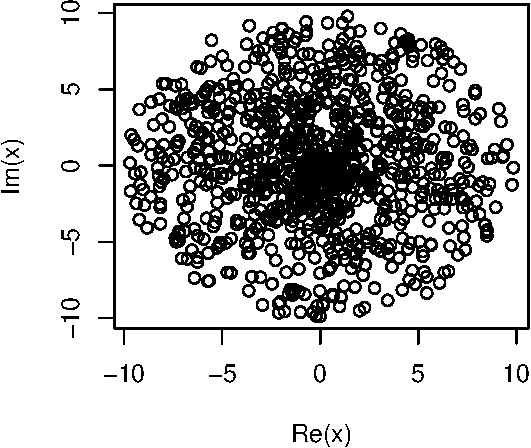
\includegraphics{Svetunkov---Svetunkov---Complex-Dynamic-Models_files/figure-latex/crvGeneratedCircle-1.pdf}
\caption{\label{fig:crvGeneratedCircle}C.r.v. generated from a uniform distribuiton.}
\end{figure}

The example in Figure \ref{fig:crvGeneratedCircle} demonstrates how a c.r.v. with uncorrelated real and imaginary parts looks on the complex plane. If there is a relation between the parts then the circle transforms into ellipse. So, it is only logical to consider the distributions that rely on a circle or an ellipse for the c.r.v. instead of any other geometric shapes.

When it comes to distribution functions, in case of c.r.v. in general we should consider the joint bivariate distribution, thus all the probability density and cumulative distribution functions will be plotted in 3D with the density/probability in z-axis and the complex variable in x and y axes.

\hypertarget{distributionCNorm}{%
\subsection{Complex Normal distribution}\label{distributionCNorm}}

One of the most popular distributions in statistics is the Normal distribution. There exists a complex counterpart of that distribution, which has the following probability density function \citep{refGoodman}:
\begin{equation}
    f(\underline{x}) = \frac{1}{\pi^2 \sqrt{\sigma^4 - \varsigma^2 \tilde{\varsigma}^2}} \exp\left(- \frac{1}{2}
        \begin{pmatrix} \underline{\tilde{x}} - \underline{\tilde{\mu}} & \underline{x} - \underline{\mu} \end{pmatrix}
        \begin{pmatrix} \sigma^2 & \varsigma^2 \\ \tilde{\varsigma}^2 & \sigma^2 \end{pmatrix}^{-1}
        \begin{pmatrix} \underline{x} - \underline{\mu} \\ \underline{\tilde{x}} - \underline{\tilde{\mu}} \end{pmatrix}
    \right),
    \label{eq:ComplexNormalPDF}
\end{equation}
where \(\underline{\mu}\) is the first moment of the c.r.v. \(\underline{x}\) and \(\sigma^2\) and \(\varsigma^2\) are the conjugate and direct variances as defined in Section \ref{complexRandomVariable}. The variable that follows this distribution can be denoted as \(\underline{x} \sim \mathcal{CN}(\underline{\mu}, \sigma^2, \varsigma^2)\) Note that both \(\sigma^2\) and \(\varsigma^2\) are important in the PDF \eqref{eq:ComplexNormalPDF} to define the shape of the distribution. For the real-valued variables, the conventional standard deviation \(\sigma\) characterises the dispersion of the random variable, and in case of the normal distribution shows how many z-scores away the random variable can lie from its centre. For the c.r.v., \(\sigma\) plays a similar role, but not in terms of units along the x axis, but rather in terms of radii from the centre. The direct variance \(\varsigma^2\), on the other hand characterises the shape of the distribution itself: its real part shows whether the ellipse of the normal distribution should be wide (positive numbers) or narrow (negative numbers), while the imaginary part shows how close the points should be to the line drawn through them. These moments are shown visually in Figure \ref{fig:crvNormalMoments}.

\begin{figure}
\centering
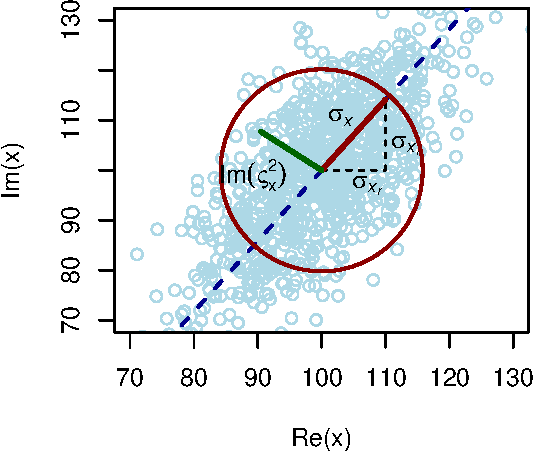
\includegraphics{Svetunkov---Svetunkov---Complex-Dynamic-Models_files/figure-latex/crvNormalMoments-1.pdf}
\caption{\label{fig:crvNormalMoments}Visual representation of variances for a c.r.v. that follows Complex Normal distribution.}
\end{figure}

The overall conjugate standard deviation \(\sigma_x\) represents the radius of the unit circle in Figure \ref{fig:crvNormalMoments}, while the imaginary part of \(\varsigma_x^2\) (i.e.~\(2 \sigma_{x_r, x_i}\)) is shown with a green line. The real part of \(\varsigma_x^2\) is not visualised, but for this plot it will be negative, showing that the distribution is narrower along the x-axis than along the y-axis.

Figure \ref{fig:plotlyCNormal} shows the PDF of \(x \sim \mathcal{CN}(100+100i,100,-20+i30)\), while Figure \ref{fig:plotlyCNormalHeatmap} shows the heatmap of the same PDF. The brighter areas in both Figures correspond to the higher values of PDF. For each specific value of density, there is a multitude of values of \(x\), forming an ellipse of a specific length.

\begin{figure}
\centering
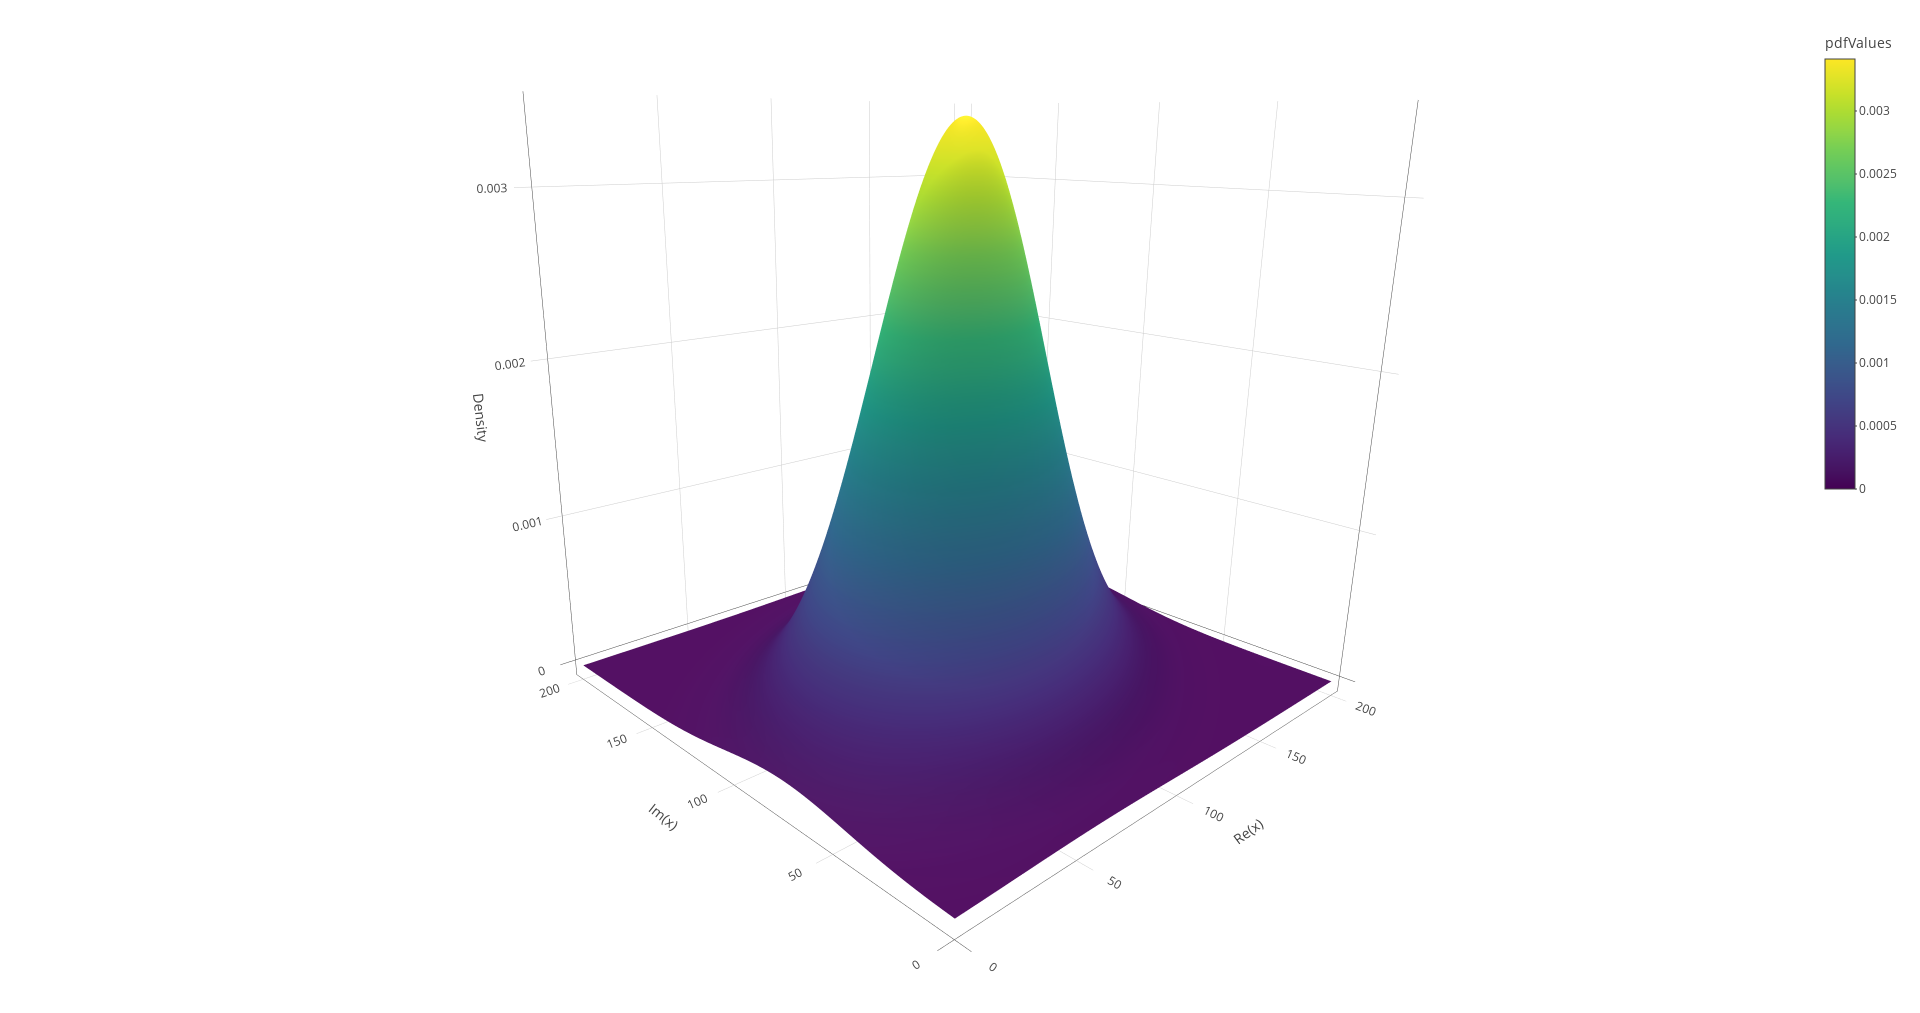
\includegraphics{./images/plotlyCNormal.png}
\caption{\label{fig:plotlyCNormal}Plot of the probability density function of complex normal distribution.}
\end{figure}

\begin{figure}
\centering
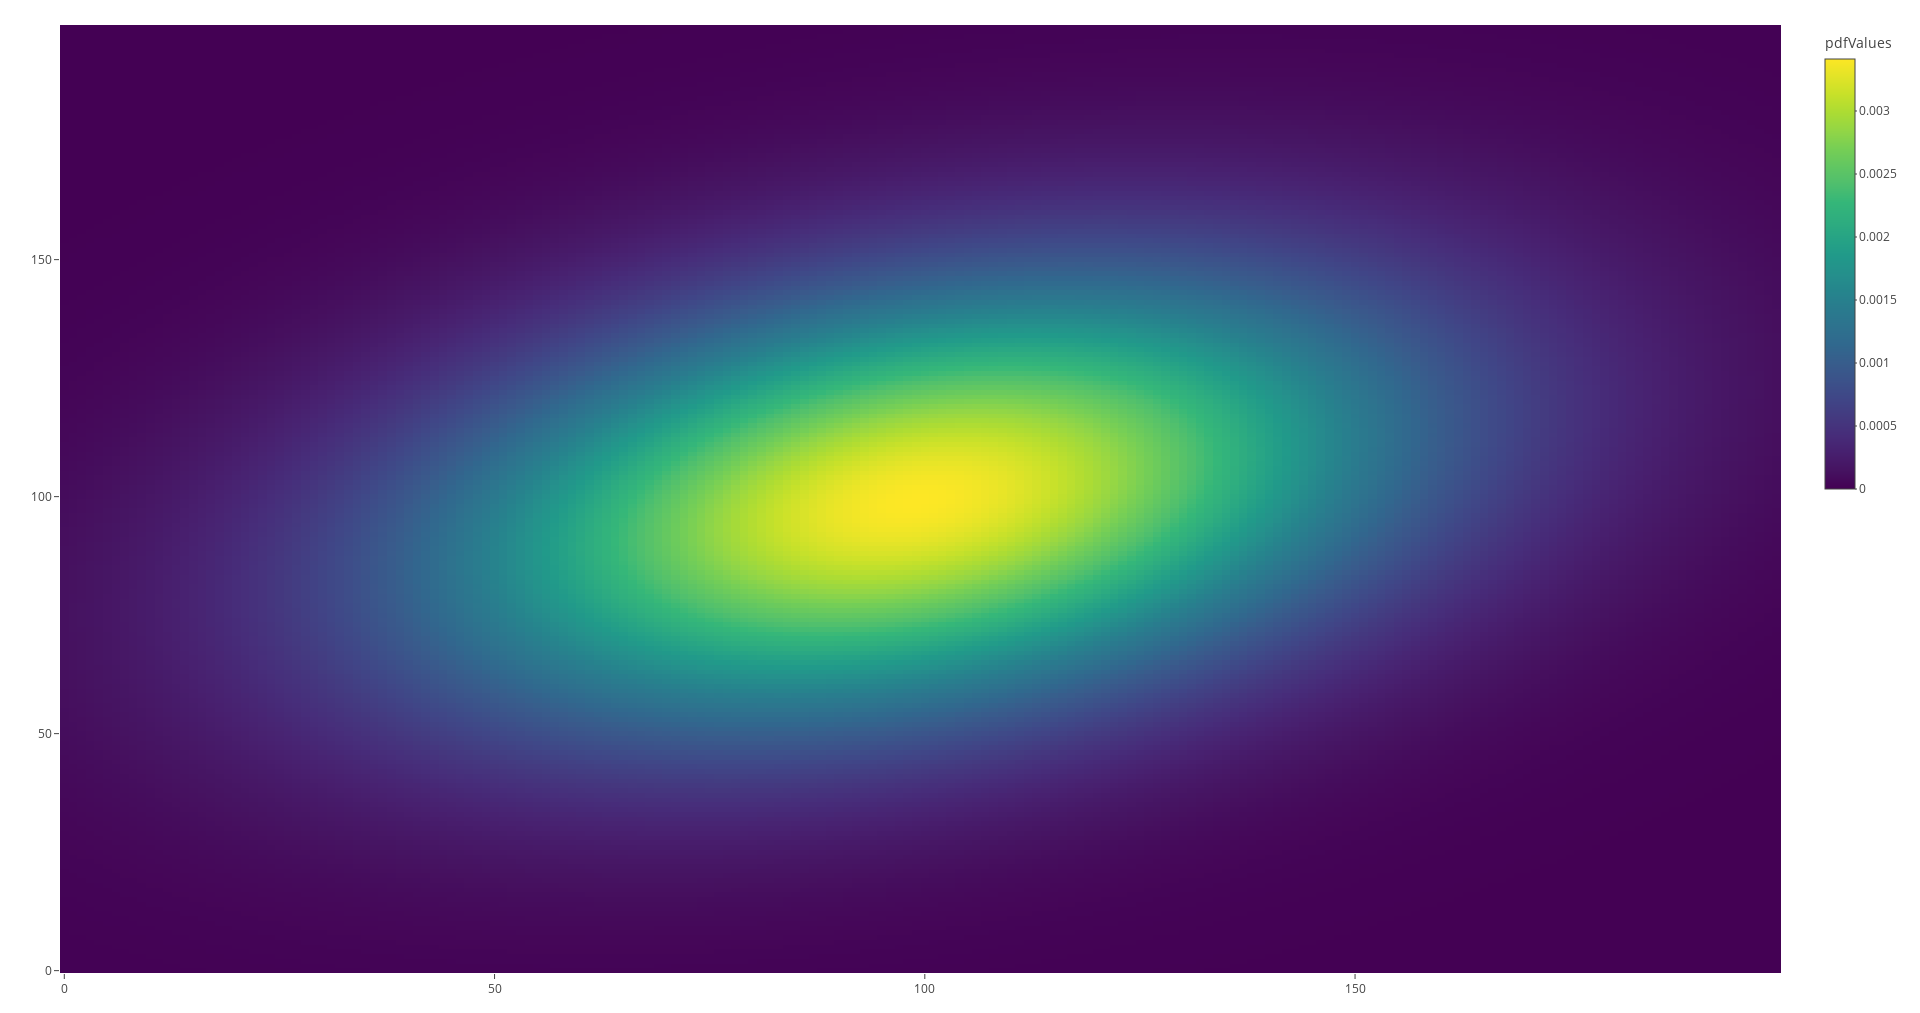
\includegraphics{./images/plotlyCNormalHeatmap.png}
\caption{\label{fig:plotlyCNormalHeatmap}Heatmap of density of Complex Normal distribution.}
\end{figure}

One special case of a Complex Normal distribution is a so called ``Circular Symmetric'' Complex Normal distribution. It is a distribution for which the direct variance equals to zero, which implies that the variances of the real and the imaginary parts are equal and that the covariance between them is equal to zero. This specific distribution is used extensively in signal processing literature \citep{referenceHere}.

The functions of the Complex Normal distribution are implemented as \texttt{dcnorm()}, \texttt{pcnorm()}, \texttt{qmcnorm()} and \texttt{rmcnorm()} in the \texttt{complex} package.

The Complex Normal distribution can be used for the joint estimation of parameters of a complex-valued model and for generation of prediction intervals from it. However, in some cases it might be more convenient to consider a c.r.v. model as a bivariate vector model based on \eqref{eq:complexFunctionVectors} and thus to revert to the multivariate normal distribution.

\hypertarget{multivariate-normal-distribution}{%
\subsection{Multivariate Normal distribution}\label{multivariate-normal-distribution}}

The same normal distribution for a complex variable can be parametrised via a covariance matrix \(\boldsymbol{\Sigma}\) from \eqref{eq:crvMomentSecondVarianceMatrix} instead of the conjugate and direct variances \(\sigma^2\) and \(\varsigma^2\). In general, the Probability Density Function for a vector of \(n\) variables can be written as:
\begin{equation}
    f(\mathbf{x}) = \frac{1}{(2 \pi)^{\frac{n}{2}} \sqrt{|\boldsymbol{\Sigma}|}} \exp\left(- \frac{1}{2}
        \begin{pmatrix} \mathbf{x} - \boldsymbol{\mu} \end{pmatrix}^\top \boldsymbol{\Sigma}^{-1} \begin{pmatrix} \mathbf{x} - \boldsymbol{\mu} \end{pmatrix}
    \right).
    \label{eq:MultivariateNormalPDF}
\end{equation}
For the bivariate case of a c.r.v. represented in a form of a vector, \(n=2\) and the covariance matrix \(\boldsymbol{\Sigma}\) has dimensionality of \(2 \times 2\). In that case the PDF will be the same as for the Complex Normal distribution. In fact, it is possible to recreate the covariance matrix based on the values of conjugate and direct variances:
\begin{equation}
    \boldsymbol{\Sigma} = \frac{1}{2} \begin{pmatrix} \sigma^2 + \mathcal{R}(\varsigma^2) & \mathcal{I}(\varsigma^2) \\
                                                      \mathcal{I}(\varsigma^2) & \sigma^2 - \mathcal{R}(\varsigma^2) \end{pmatrix} .
    \label{eq:MultivariateNormalPDFCovariance}
\end{equation}

When it comes to constructing confidence regions from the multivariate normal distribution then the following inequality is used to determine values of the vector of quantiles \(\mathbf{q}\):
\begin{equation}
    (\mathbf{x} - \mathbf{q})^{\top} \mathbf{\Sigma}^{-1} (\mathbf{x} - \mathbf{q}) \leq \chi^2(n, p) ,
    \label{eq:MultivariateNormalRegion}
\end{equation}
where \(p\) is the confidence level. For the case of c.r.v., when \(n=2\), the \(\chi^2(n, p)\) transforms into the exponential distribution \(\mathcal{E}(0.5)\).

Note however that working with confidence regions is challenging, because there is an infinite number of values of the vector \(\mathbf{q}\) that give the same critical value \(\chi^2(n, p)\). So, in order to make it practical, unconditional prediction intervals can be constructed for each of the parts, dropping the other one. In this case, the classical formula for the intervals can be used, for example for the real part of the c.r.v.:
\begin{equation}
    x_{r} \in \left( \mu_{x_r} + \sigma_{x_r} z \left({\frac{\alpha}{2}} \right) , \mu_{x_r} + \sigma_{x_r} z \left({\frac{1+\alpha}{2}} \right) \right),
    \label{eq:NormalInterval}
\end{equation}
where \(z\left({\frac{\alpha}{2}} \right)\) and \(z\left({\frac{1+\alpha}{2}} \right)\) are the respective lower and upper quantiles of the standard normal distribution.

\hypertarget{hotellings-t-squared-distribution}{%
\subsection{Hotelling's T-squared distribution}\label{hotellings-t-squared-distribution}}

When it comes to distribution of complex variables statistics, one of the most important ones is a distribution of a mean of a complex variable. In the case of real variables, it is well known that if the Central Limit Theorem (CLT) holds then the sample mean will follow Normal distribution, and confidence interval for the mean can be constructed using Student's t distribution (when the population variance is unknown, i.e.~in reality). For c.r.v., the situation is similar: when CLT holds, the c.r.v. follows Complex Normal distribution, but instead of Student's t distribution, we need to use its multivariate counterpart, which is called ``Hotelling's T-squared'' distribution. It is more convenient to consider the statistics for a c.r.v in a vector form (i.e.~treat it as bivariate). If we estimate the sample mean \(\hat{\boldsymbol{\mu}}_x\) and a sample covariance matrix of the mean \(\hat{\boldsymbol{\Sigma}}_{\mu_{x}}\) then the following holds (if CLT holds):
\begin{equation}
    (\hat{\boldsymbol{\mu}}_x - \boldsymbol{\mu}_x)^\prime \hat{\boldsymbol{\Sigma}}_{\mu_{x}}^{-1} (\hat{\boldsymbol{\mu}}_x - \boldsymbol{\mu}_x) \sim T^2(2, n-1) = \frac{2(n-1)}{n-2} F(2, n-2),
    \label{eq:hotellingT}
\end{equation}
where \(T^2(2, n-1)\) is a T-squared Hotelling's statistics with 2 and \(n-1\) degrees of freedom, and \(F(2, n-2)\) is the Fisher's distribution statistics with 2 and \(n-2\) degrees of freedom. Equation \eqref{eq:hotellingT} can be used to construct confidence interval for a multivariate mean or for testing statistical hypotheses. One of the possible hypotheses that would make sense in case of c.r.v. and could be tested based on \eqref{eq:hotellingT} is the following:
\begin{equation}
    \begin{aligned}
        & \mathrm{H}_0: \boldsymbol{\mu}_x = 0 \\
        & \mathrm{H}_1: \boldsymbol{\mu}_x \neq 0
    \end{aligned}
    \label{eq:hypothesisFirst}
\end{equation}
or equivalently:
\begin{equation}
    \begin{aligned}
        & \mathrm{H}_0: \mu_{x_r} = \mu_{x_i} = 0 \\
        & \mathrm{H}_1: \mu_{x_r} \neq 0 \vee \mu_{x_i} \neq 0
    \end{aligned}
    \label{eq:hypothesisSecond}
\end{equation}
However, from practical point of view, testing the joint hypothesis \eqref{eq:hypothesisSecond} might not be very useful. Instead, testing the classical hypotheses from the univariate context based on Student's t distribution might provide more detailed information, i.e.~whether the specific real or imaginary part of the variable equals to zero or not. In contrast, in case of the hypothesis \eqref{eq:hypothesisSecond}, rejecting the null hypothesis implies that something is not equal to zero, but it is not clear, what specifically.

\hypertarget{simpleCLR}{%
\chapter{Simple Complex Linear Regression}\label{simpleCLR}}

We start with the simplest Complex Linear Regression (CLR), which we call ``simple'', because it captures the relation between two variables. The main difference from the conventional Simple Linear Regression is that each of the variables is complex. This makes the model more complicated than the one in real numbers domain.

\hypertarget{simpleCLRModel}{%
\section{Model formulation}\label{simpleCLRModel}}

The simple Complex Linear Regression can be written as:
\begin{equation}
    \underline{y_j} = \underline{\beta_0} + \underline{\beta_1} \underline{x_j} + \underline{\epsilon_j},
    \label{eq:SimpleCLRComplex}
\end{equation}
where \(j\) is the index for an observation and every parameter and variable is a complex number, i.e.~\(\underline{y_j} = y_{r,j}+i y_{i,j}\) is the complex response variable, \(\underline{x_j} = x_{r,j}+i x_{i,j}\) is the complex explanatory variable, \(\underline{\beta_{l}} = \beta_{l,r} + i \beta_{l,i}\) is the \(l\)-th parameter and \(\underline{\epsilon_j} = \epsilon_{r,j} + i \epsilon_{i,j}\) is the error term. For now, we do not make any specific assumptions about the distribution of the complex error term, we will come back to this later in this chapter. Inserting these values in \eqref{eq:SimpleCLRComplex} leads to:
\begin{equation}
    y_{r,j}+i y_{i,j} = (\beta_{0,r} + i \beta_{0,i}) + (\beta_{1,r} + i \beta_{1,i}) (x_{r,j}+i x_{i,j}) + (\epsilon_{r,j} + i \epsilon_{i,j}),
    \label{eq:SimpleCLR}
\end{equation}
which is in fact a multivariate model, capturing how the change of values in pair of variables \(x_r\), \(x_i\) leads to the change in the pair of variables \(y_r\) and \(y_i\). Given that any complex equation can be represented as a system of two equations, the model \eqref{eq:SimpleCLR} can be represented as a system of two linear regressions:
\begin{equation}
    \begin{aligned}
        y_{r,j} = & \beta_{0,r} + \beta_{1,r} x_{r,j} - \beta_{1,i} x_{i,j} + \epsilon_{r,j} \\
        y_{i,j} = & \beta_{0,i} + \beta_{1,r} x_{i,j} + \beta_{1,i} x_{r,j} + \epsilon_{i,j}
    \end{aligned}
    \label{eq:SimpleCLRSystem}
\end{equation}
This model captures a very specific dynamics between the real and imaginary parts, given that they share the same set of parameters for the slope. But most importantly it shows how each complex variable \(y\) relates to variable \(x\) in a four dimensional space. Note that the real and imaginary parts of \(y\) can be exchanged without a serious impact on the model: in that case the values of parameters would change, but the relation between \(x\) and \(y\) would stay the same. Similarly, changing \(x_r\) with \(x_i\) would only lead to different estimates of parameters, the general relation will hold.

Given that we deal with a sample of values, the model \eqref{eq:SimpleCLRComplex} can be represented in a vector form for all observations \(j\) from 1 to \(n\) (based on discussion in Subsection \ref{vectorComplexVariables}):
\begin{equation}
    \underline{\mathbf{y}} = \underline{\mathbf{X}} \underline{\boldsymbol{\beta}} + \underline{\boldsymbol{\epsilon}} ,
    \label{eq:SimpleCLRVector}
\end{equation}
where \(\underline{\mathbf{y}}=\begin{pmatrix} \underline{{y}_1} \\ \underline{{y}_2} \\ \vdots \\ \underline{{y}_n} \end{pmatrix}\), \(\underline{\mathbf{X}} = \begin{pmatrix} 1 & \underline{{x}_1} \\ 1 & \underline{{x}_2}\\ \vdots \\ 1 & \underline{{x}_n} \end{pmatrix}\), \(\underline{\boldsymbol{\beta}} = \begin{pmatrix} \underline{{\beta}_0} \\ \underline{{\beta}_1} \end{pmatrix}\) and \(\underline{\boldsymbol{\epsilon}} = \begin{pmatrix} \underline{{\epsilon}_1} \\ \underline{{\epsilon}_2}\\ \vdots \\ \underline{{\epsilon}_n} \end{pmatrix}\), where each element of the objects above is a complex number.

Going even further, using the vector and matrix representations of complex variables, the same system of equations \eqref{eq:SimpleCLRSystem} can be rewritten as:
\begin{equation}
    \begin{pmatrix} y_{r,j} \\ y_{i,j} \end{pmatrix} = \begin{pmatrix} \beta_{0,r} \\ \beta_{0,i} \end{pmatrix} + \begin{pmatrix} x_{r,j} & -x_{i,j} \\ x_{i,j} & x_{r,j} \end{pmatrix} \begin{pmatrix} \beta_{1,r} \\ \beta_{1,i} \end{pmatrix} + \begin{pmatrix} \epsilon_{r,j} \\ \epsilon_{i,j} \end{pmatrix} ,
    \label{eq:SimpleCLRSystemVector01}
\end{equation}
or uniting all the parameters in one vector:
\begin{equation}
    \begin{pmatrix} y_{r,j} \\ y_{i,j} \end{pmatrix} = \begin{pmatrix} 1 & 0 & x_{r,j} & -x_{i,j} \\ 0 & 1 & x_{i,j} & x_{r,j} \end{pmatrix} \begin{pmatrix} \beta_{0,r} \\ \beta_{0,i} \\ \beta_{1,r} \\ \beta_{1,i} \end{pmatrix} + \begin{pmatrix} \epsilon_{r,j} \\ \epsilon_{i,j} \end{pmatrix} .
    \label{eq:SimpleCLRSystemVector02}
\end{equation}

This form can then be represented in a classical matrix notations:
\begin{equation}
    \mathbf{y}_j = \underset{\sim}{\mathbf{X}_j} {\boldsymbol{\beta}} + \boldsymbol{\epsilon}_j .
    \label{eq:SimpleCLRSystemVector03}
\end{equation}
And if we stack each of the vectors and matrices for each \(j=1 \dots n\) we get even more compact form:
\begin{equation}
    \mathbf{Y} = \underset{\sim}{\mathbf{X}} \boldsymbol{\beta} + \mathbf{E} ,
    \label{eq:SimpleCLRSystemVectorFinal}
\end{equation}
where \(\mathbf{Y}=\begin{pmatrix}\mathbf{y}_1 \\ \mathbf{y}_2\\ \vdots \\ \mathbf{y}_n \end{pmatrix}\), \(\underset{\sim}{\mathbf{X}}=\begin{pmatrix} \underset{\sim}{\mathbf{X}_1} \\ \underset{\sim}{\mathbf{X}_2} \\ \vdots \\ \underset{\sim}{\mathbf{X}_n} \end{pmatrix}\) and \(\mathbf{E}=\begin{pmatrix}\boldsymbol{\epsilon}_1 \\ \boldsymbol{\epsilon}_2\\ \vdots \\ \boldsymbol{\epsilon}_n \end{pmatrix}\). The form \eqref{eq:SimpleCLRSystemVectorFinal} shows the connection between the complex regression and the conventional real valued one. As it can be seen, they both can be represented in matrix forms, which means that some of the approaches used for the latter can be transferred to the former under some conditions.

\hypertarget{SCLREstimation}{%
\section{Estimation}\label{SCLREstimation}}

Whenever we estimate a model, we substitute the ``true'' parameters by their sample estimates. So, for the CLR, the model applied to the data should be written as:
\begin{equation}
    \underline{y_j} = \underline{b_0} + \underline{b_1} \underline{x_j} + \underline{e_j},
    \label{eq:SimpleCLRComplexEstimated}
\end{equation}
or
\begin{equation}
    y_{r,j}+i y_{i,j} = (b_{0,r} + i b_{0,i}) + (b_{1,r} + i b_{1,i}) (x_{r,j}+i x_{i,j}) + (e_{r,j} + i e_{i,j}),
    \label{eq:SimpleCLREstimated}
\end{equation}
or
\begin{equation}
    \begin{aligned}
        y_{r,j} = & b_{0,r} + b_{1,r} x_{r,j} - b_{1,i} x_{i,j} + e_{r,j} \\
        y_{i,j} = & b_{0,i} + b_{1,r} x_{i,j} + b_{1,i} x_{r,j} + e_{i,j}
    \end{aligned}
    \label{eq:SimpleCLRSystemEstimated}
\end{equation}
or equivalently in matrix notations:
\begin{equation}
    \mathbf{y}_j = \underset{\sim}{\mathbf{X}_j} \boldsymbol{b} + \boldsymbol{e}_j ,
    \label{eq:SimpleCLRSystemVector03Estimated}
\end{equation}
where \(\underline{b_{l}}\), \(b_{l,r}+ib_{l,i}\) and \(\boldsymbol{b}\) are the estimates of respective \(\underline{\beta_l}\), \(\beta_{l,r} + i \beta_{l,i}\) and \(\boldsymbol{\beta}\) and \(\underline{e_j}\), \(e_{r,j} + i e_{i,j}\) and \(\boldsymbol{e}_j\) are the residuals of the model. Now in order to get estimates of parameters, we can use one of several approaches.

\hypertarget{ordinary-least-squares}{%
\subsection{Ordinary Least Squares}\label{ordinary-least-squares}}

We start with the conventional Ordinary Least Squares (OLS), which relies on the multiplication by conjugate number. For the simple CLR, it comes to minimising the following loss based on the residuals:
\begin{equation}
    \sum_{j=1}^n (\underline{e_j} \underline{\tilde{e}_j}) = \sum_{j=1}^n (e_{r,j}^2 + e_{i,j}^2).
    \label{eq:SimpleCLROLSLoss}
\end{equation}
The residuals can be substituted as: \(\underline{e_j} = \underline{y_j} - \underline{b_0} - \underline{b_1} \underline{x_j}\) and \(\underline{\tilde{e}_j} = \underline{\tilde{y}_j} - \underline{\tilde{b}_0} - \underline{\tilde{b}_1} \underline{\tilde{x}_j}\) to get:
\begin{equation}
    \sum_{j=1}^n (\underline{y_j} - \underline{b_0} - \underline{b_1} \underline{x_j}) (\underline{\tilde{y}_j} - \underline{\tilde{b}_0} - \underline{\tilde{b}_1} \underline{\tilde{x}_j}),
    \label{eq:SimpleCLROLSLoss01}
\end{equation}
which after opening the brackets becomes:
\begin{equation}
    \sum_{j=1}^n \left(\underline{y_j} \underline{\tilde{y}_j} - \underline{y_j} \underline{\tilde{b}_0} - \underline{y_j} \underline{\tilde{b}_1} \underline{\tilde{x}_j} - \underline{b_0}\underline{\tilde{y}_j} + \underline{b_0} \underline{\tilde{b}_0} + \underline{b_0} \underline{\tilde{b}_1} \underline{\tilde{x}_j} - \underline{b_1} \underline{x_j} \underline{\tilde{y}_j} + \underline{b_1} \underline{x_j} \underline{\tilde{b}_0} + \underline{b_1} \underline{x_j} \underline{\tilde{b}_1} \underline{\tilde{x}_j} \right) .
    \label{eq:SimpleCLROLSLoss02}
\end{equation}
In order to minimise the sum of squared errors \eqref{eq:SimpleCLROLSLoss}, we need to take derivative of \eqref{eq:SimpleCLROLSLoss02} with respect to each of the parameters \(b_{0,r}\), \(b_{0,i}\), \(b_{1,r}\) and \(b_{1,i}\) and equate each of the resulting equations to zero to find the extrema:
\begin{equation}
    \begin{aligned}
        & \frac{d \sum_{j=1}^n (\underline{e_j} \underline{\tilde{e}_j})}{d b_{0,r}} = 0 \\
        & \frac{d \sum_{j=1}^n (\underline{e_j} \underline{\tilde{e}_j})}{d b_{0,i}} = 0 \\
        & \frac{d \sum_{j=1}^n (\underline{e_j} \underline{\tilde{e}_j})}{d b_{1,r}} = 0 \\
        & \frac{d \sum_{j=1}^n (\underline{e_j} \underline{\tilde{e}_j})}{d b_{1,i}} = 0
    \end{aligned}
    \label{eq:SimpleCLROLSLossSystem01}
\end{equation}
to get:
\begin{equation}
    \begin{aligned}
        & - \sum_{j=1}^n \underline{y_j} - \sum_{j=1}^n \underline{\tilde{y}_j} + 2 n b_{0,r} + \underline{\tilde{b}_1} \sum_{j=1}^n \underline{\tilde{x}_j} + \underline{b_1} \sum_{j=1}^n {x}_j = 0 \\
        & i \sum_{j=1}^n \underline{y_j} - i \sum_{j=1}^n \underline{\tilde{y}_j} + 2 n b_{0,i} + i \underline{\tilde{b}_1} \sum_{j=1}^n \underline{\tilde{x}_j} - i \underline{b_1} \sum_{j=1}^n {x}_j = 0 \\
        & - \sum_{j=1}^n \underline{y_j} \underline{\tilde{x}_j} + \underline{b_0} \sum_{j=1}^n \underline{\tilde{x}_j} - \sum_{j=1}^n \underline{x_j} \underline{\tilde{y}_j} + \underline{\tilde{b}_0} \sum_{j=1}^n {x}_j + 2 b_{1,r} \sum_{j=1}^n \underline{x_j} \underline{\tilde{x}_j} = 0 \\
        & i \sum_{j=1}^n \underline{y_j} \underline{\tilde{x}_j} - i \underline{b_0} \sum_{j=1}^n \underline{\tilde{x}_j} - i \sum_{j=1}^n \underline{x_j} \underline{\tilde{y}_j} + i \underline{\tilde{b}_0} \sum_{j=1}^n {x}_j + 2 b_{1,i} \sum_{j=1}^n \underline{x_j} \underline{\tilde{x}_j} = 0 .
    \end{aligned}
    \label{eq:SimpleCLROLSLossSystem02}
\end{equation}
As shown by \citet{Svetunkov2012}, solving the system of equations \eqref{eq:SimpleCLROLSLossSystem02} gives the following formulae for the parameters of the model:
\begin{equation}
    \begin{aligned}
        & \underline{b_1} = \frac{\sum_{j=1}^n (\underline{y_j}-\underline{\hat{\mu}_{y}}) (\underline{\tilde{x}_j}-\hat{\tilde{\mu}}_{x})}{\sum_{j=1}^n (\underline{{x}_j}-\underline{\hat{\mu}_{x}}) (\underline{\tilde{x}_j}-\hat{\tilde{\mu}}_{x})} \\
        & \underline{b_0} = \frac{1}{n} \sum_{j=1}^n \underline{y_j} - \underline{b_1} \sum_{j=1}^n \underline{x_j} ,
    \end{aligned}
    \label{eq:SimpleCLROLSLossParameters}
\end{equation}
which can also be written in terms of conjugate moments as:
\begin{equation}
    \begin{aligned}
        & \underline{b_1} = \frac{\hat{\sigma}_{x,y}}{\hat{\sigma}_x^2} \\
        & \underline{b_0} = \underline{\hat{\mu}_{y}} - \underline{b_1} \underline{\hat{\mu}_{x}} .
    \end{aligned}
    \label{eq:SimpleCLROLSLossParametersMoments}
\end{equation}
or after expanding the moments (based on formulae from Section \ref{crvSecondMoment}) as:
\begin{equation}
        \underline{b_1} = \frac{\hat{\sigma}_{x_r, y_r} + \hat{\sigma}_{x_i, y_i} + i (\hat{\sigma}_{x_r, y_i} - \hat{\sigma}_{x_i, y_r})}{\hat{\sigma}_{x_r}^2 + \hat{\sigma}_{x_i}^2}
    \label{eq:SimpleCLROLSLossParametersMomentsExpanded}
\end{equation}

As we can see, the formula \eqref{eq:SimpleCLROLSLossParametersMoments} is similar to the one that is typically used for the conventional simple linear regression with the only difference that the parameters in \eqref{eq:SimpleCLROLSLossParametersMoments} are complex and that each of the moments in \eqref{eq:SimpleCLROLSLossParametersMoments} is a moment for respective complex variable.

It is apparent what the estimates of parameters \eqref{eq:SimpleCLROLSLossParametersMoments} correspond to: they minimise the loss \eqref{eq:SimpleCLROLSLoss}, thus in the case, when \(\mathrm{E}(\underline{e_j})=0\) they minimise variances of real and imaginary parts of the complex residuals. A thing to note is that they ignore the potential covariance between them, which in some cases might be a desirable property, but in the others might cause issues.

In terms of properties of the estimator, it can be shown that \(\underline{b_1}\) equals to:
\begin{equation}
        \underline{b_1} = \frac{\mathrm{cov}(\underline{\tilde{x}}, \underline{y})}{\mathrm{cov}(\underline{\tilde{x}},\underline{x})} = \frac{\mathrm{cov}(\underline{\tilde{x}}, \underline{\beta_0} + \underline{\beta_1} \underline{x} + \underline{\epsilon})}{\mathrm{cov}(\underline{\tilde{x}},\underline{x})} = \frac{\mathrm{cov}(\underline{\tilde{x}}, \underline{\beta_0}) + \mathrm{cov}(\underline{\tilde{x}}, \underline{\beta_1} \underline{x}) + \mathrm{cov}(\underline{\tilde{x}}, \underline{\epsilon})}{\mathrm{cov}(\underline{\tilde{x}},\underline{x})},
    \label{eq:SimpleCLROLSb1Value01}
\end{equation}
which then simplifies to:
\begin{equation}
        \underline{b_1} = \underline{\beta_1} + \frac{\mathrm{cov}(\underline{\tilde{x}}, \underline{\epsilon})}{\mathrm{cov}(\underline{\tilde{x}},\underline{x})} = \underline{\beta_1} + \frac{\hat{\sigma}_{x,\epsilon}}{\hat{\sigma}_x^2} ,
    \label{eq:SimpleCLROLSb1Value02}
\end{equation}
or:
\begin{equation}
        \underline{b_1} = \underline{\beta_1} + \frac{\hat{\sigma}_{x_r, \epsilon_r} + \hat{\sigma}_{x_i, \epsilon_i} + i (\hat{\sigma}_{x_r, \epsilon_i} - \hat{\sigma}_{x_i, \epsilon_r})}{\hat{\sigma}_{x_r}^2 + \hat{\sigma}_{x_i}^2} .
    \label{eq:SimpleCLROLSb1Value03}
\end{equation}
On small samples, the covariance between the true error and the available \(\underline{x}\) can be not equal to zero, implying that the value of the estimated parameter would differ from the true one. If the basic regression assumptions hold, in the population estimated covariances will converge to their true values and then \({\sigma}_{x_r, \epsilon_r} = {\sigma}_{x_i, \epsilon_i} = {\sigma}_{x_r, \epsilon_i} = {\sigma}_{x_i, \epsilon_r}=0\), which implies that the expectation of \(\underline{b_1}\) is:
\begin{equation}
        \mathrm{E}(\underline{b_1}) = \underline{\beta_1} .
    \label{eq:SimpleCLROLSb1Expectation}
\end{equation}
This implies that OLS gives unbiased estimates of the slope parameter. The same property can be shown to hold for the intercept \(\underline{b_0}\).

The same formula \eqref{eq:SimpleCLROLSb1Value03} can be rewritten separately for the real and imaginary parts of the parameter:
\begin{equation}
    \begin{aligned}
        b_{1,r} = & \beta_{1,r} + \frac{\hat{\sigma}_{x_r, \epsilon_r} + \hat{\sigma}_{x_i, \epsilon_i}}{\hat{\sigma}_{x_r}^2 + \hat{\sigma}_{x_i}^2} \\
        b_{1,i} = & \beta_{1,i} + \frac{\hat{\sigma}_{x_r, \epsilon_i} - \hat{\sigma}_{x_i, \epsilon_r}}{\hat{\sigma}_{x_r}^2 + \hat{\sigma}_{x_i}^2} ,
    \end{aligned}
    \label{eq:SimpleCLROLSb1Value04}
\end{equation}
which shows what specific covariances impact different parts of the slope parameter.

As for the variance of \(\underline{b_1}\), for the real part of the parameter, it can be shown to be equal to:
\begin{equation}
    \mathrm{V}(b_{1,r}) = \mathrm{V}\left(\frac{\hat{\sigma}_{x_r, \epsilon_r} + \hat{\sigma}_{x_i, \epsilon_i}}{\hat{\sigma}_{x_r}^2 + \hat{\sigma}_{x_i}^2}\right) .
    \label{eq:SimpleCLROLSb1Variance}
\end{equation}
The variance for the imaginary part will be similar. We do not expand it further, because the formula \eqref{eq:SimpleCLROLSb1Variance} is sufficient for the comparison of OLS with other estimators.

\hypertarget{SCLREstimationCLS}{%
\subsection{Complex Least Squares}\label{SCLREstimationCLS}}

An alternative estimation technique involves the minimisation of a rather exotic loss function:
\begin{equation}
    \sum_{j=1}^n (\underline{e_j} \underline{e_j}) = \sum_{j=1}^n (e_{r,j}^2 - e_{i,j}^2 + i 2 e_{r,j} e_{i,j}),
    \label{eq:SimpleCLRCLSLoss}
\end{equation}
for which in case of \(\mathrm{E}(\underline{e_j})=0\), the real part corresponds to the difference between the variances of the real and imaginary parts of the residuals, while the imaginary parts corresponds to the covariance between them. This loss be considered exotic, because its value is a complex number. It is difficult to explain how one can minimise a complex number, but from what follows, we show that the estimation technique has some meaning, works and gives adequate estimates of parameters.

The logic for the derivation of CLS is similar to OLS. We expand \eqref{eq:SimpleCLRCLSLoss} to:
\begin{equation}
    \sum_{j=1}^n (\underline{e_j} \underline{e_j}) = \sum_{j=1}^n \underline{y_j}^2 + n \underline{b_0}^2 + \underline{b_1}^2 \sum_{j=1}^n \underline{x_j}^2 - 2 \underline{b_0} \sum_{j=1}^n \underline{y_j} - 2 \underline{b_1} \sum_{j=1}^n \underline{x_j} \underline{y_j} + 2 \underline{b_0} \underline{b_1} \sum_{j=1}^n \underline{x_j} 
    \label{eq:SimpleCLRCLSLoss02}
\end{equation}
and then take derivatives of \eqref{eq:SimpleCLRCLSLoss02} with respect to parameter \(\underline{b_0}\) and \(\underline{b_1}\) and then equate the resulting equations to zero:
\begin{equation}
    \begin{aligned}
        & \frac{d \sum_{j=1}^n (\underline{e_j}^2)}{d \underline{b_0}} = 0 \\
        & \frac{d \sum_{j=1}^n (\underline{e_j}^2)}{d \underline{b_1}} = 0 .
    \end{aligned}
    \label{eq:SimpleCLRCLSLossSystem01}
\end{equation}
The derivatives \eqref{eq:SimpleCLRCLSLossSystem01} give the following system of complex equations:
\begin{equation}
    \begin{aligned}
        & 2 n \underline{b_0} - 2 \sum_{j=1}^n \underline{y_j} + 2 \underline{b_1} \sum_{j=1}^n \underline{x_j} = 0 \\
        & 2 \underline{b_1} \sum_{j=1}^n \underline{x_j}^2 - 2 \sum_{j=1}^n \underline{x_j} \underline{y_j} + 2 \underline{b_0} \sum_{j=1}^n \underline{x_j} = 0 .
    \end{aligned}
    \label{eq:SimpleCLRCLSLossSystem02}
\end{equation}
The solution for this system of equations, as it was shown by \citet{Svetunkov2012}, is:
\begin{equation}
    \begin{aligned}
        & \underline{b_1} = \frac{\sum_{j=1}^n (\underline{y_{j}}-\underline{\hat{\mu}_{y}}) (\underline{{x}_j}-\underline{\hat{\mu}_{x}})}{\sum_{j=1}^n (\underline{{x}_j}-\underline{\hat{\mu}_{x}})^2} \\
        & \underline{b_0} = \frac{1}{n} \sum_{j=1}^n \underline{y_j} - \underline{b_1} \sum_{j=1}^n \underline{x_j} ,
    \end{aligned}
    \label{eq:SimpleCLRCLSLossParameters}
\end{equation}
or in terms of direct moments for complex random variables:
\begin{equation}
    \begin{aligned}
        & \underline{b_1} = \frac{\hat{\varsigma}_{x,y}}{\hat{\varsigma}_x^2} \\
        & \underline{b_0} = \underline{\hat{\mu}_{y}} - \underline{b_1} \underline{\hat{\mu}_{x}} ,
    \end{aligned}
    \label{eq:SimpleCLRCLSLossParametersMoments}
\end{equation}
or after inserting the values for direct variance and covariance (from Section \ref{crvSecondMoment}):
\begin{equation}
    \begin{aligned}
        & \underline{b_1} = \frac{\hat{\sigma}_{x_r, y_r} - \hat{\sigma}_{x_i, y_i} + i (\hat{\sigma}_{x_i, y_r} + \hat{\sigma}_{x_r, y_i})}{\hat{\sigma}_{x_r}^2 - \hat{\sigma}_{x_i}^2 + i2 \hat{\sigma}_{x_r,x_i}} \\
        & \underline{b_0} = \underline{\hat{\mu}_{y}} - \underline{b_1} \underline{\hat{\mu}_{x}} .
    \end{aligned}
    \label{eq:SimpleCLRCLSLossParametersMomentsExpanded}
\end{equation}
Similarly to how it was done with OLS estimate of the slope, we can consider the estimate of \(\underline{b_1}\), expanding the covariance in the numerator of \eqref{eq:SimpleCLRCLSLossParametersMoments}:
\begin{equation}
        \underline{b_1} = \frac{\mathrm{cov}(\underline{x},\underline{y})}{V(\underline{x})} = \frac{\mathrm{cov}(\underline{x},\underline{\beta_0} + \underline{\beta_1} \underline{x} + \underline{\epsilon})}{V(\underline{x})},
    \label{eq:SimpleCLRCLSb1Expansion01}
\end{equation}
which after some simplifications becomes:
\begin{equation}
        \underline{b_1} = \underline{\beta_1} + \frac{\mathrm{cov}(\underline{x}, \underline{\epsilon})}{V(\underline{x})} ,
    \label{eq:SimpleCLRCLSb1Expansion02}
\end{equation}
which can be expanded to:
\begin{equation}
    \underline{b_1} = \underline{\beta_1} + \frac{\mathrm{cov}(x_r, \epsilon_r) - \mathrm{cov}(x_i, \epsilon_i) + i (\mathrm{cov}(x_r, \epsilon_i) + \mathrm{cov}(x_i, \epsilon_r))}{V(x_r) - V(x_i) + 2i \mathrm{cov}(x_r, x_i)} . 
    \label{eq:SimpleCLRCLSb1Expansion03}
\end{equation}
Note that both numerator and denominator of \eqref{eq:SimpleCLRCLSb1Expansion03} are complex numbers. In order to have a proper split into real and imaginary parts we need to multiply the fraction by the complex number conjugate to the denominator:
\begin{equation}
\resizebox{0.9\textwidth}{!}{$
        \underline{b_1} = \underline{\beta_1} + \frac{\left(\mathrm{cov}(x_r, \epsilon_r) - \mathrm{cov}(x_i, \epsilon_i) + i (\mathrm{cov}(x_r, \epsilon_i) + \mathrm{cov}(x_i, \epsilon_r))\right)\left(V(x_r) - V(x_i) - 2i \mathrm{cov}(x_r, x_i)\right)}{\left(V(x_r) - V(x_i)\right)^2 + 4 \mathrm{cov}(x_r, x_i)^2} $}.
    \label{eq:SimpleCLRCLSb1Expansion04}
\end{equation}
This then can be split into two parts:
\begin{equation}
\resizebox{0.9\textwidth}{!}{$
    \begin{aligned}
        b_{1,r} = & \beta_{1,r} + \frac{\left(\mathrm{cov}(x_r, \epsilon_r) - \mathrm{cov}(x_i, \epsilon_i)\right) \left(V(x_r) - V(x_i)\right) - 2 \mathrm{cov}(x_r, x_i) \left(\mathrm{cov}(x_r, \epsilon_i) + \mathrm{cov}(x_i, \epsilon_r)\right)}{\left(V(x_r) - V(x_i)\right)^2 + 4 \mathrm{cov}(x_r, x_i)^2} \\
        b_{1,i} = & \beta_{1,i} + \frac{\left( \mathrm{cov}(x_r, \epsilon_i) + \mathrm{cov}(x_i, \epsilon_r)\right)\left(V(x_r) - V(x_i) \right) + 2 \mathrm{cov}(x_r, x_i) \left(\mathrm{cov}(x_i, \epsilon_i) - \mathrm{cov}(x_r, \epsilon_r)\right)}{\left(V(x_r) - V(x_i)\right)^2 + 4 \mathrm{cov}(x_r, x_i)^2} 
    \end{aligned}$}
    \label{eq:SimpleCLRCLSb1Expansion05}
\end{equation}
or
\begin{equation}
    \begin{aligned}
        b_{1,r} = & \beta_{1,r} + \frac{\left(\hat{\sigma}_{x_r, \epsilon_r} - \hat{\sigma}_{x_i, \epsilon_i}\right) \left(\hat{\sigma}_{x_r}^2 - \hat{\sigma}_{x_i}^2 \right) - 2 \hat{\sigma}_{x_r, x_i} \left(\hat{\sigma}_{x_r, \epsilon_i} + \hat{\sigma}_{x_i, \epsilon_r}\right)}{\left(\hat{\sigma}_{x_r}^2 - \hat{\sigma}_{x_i}^2\right)^2 + 4 \hat{\sigma}_{x_r, x_i}^2} \\
        b_{1,i} = & \beta_{1,i} + \frac{\left( \hat{\sigma}_{x_r, \epsilon_i} + \hat{\sigma}_{x_i, \epsilon_r}\right)\left(\hat{\sigma}_{x_r}^2 - \hat{\sigma}_{x_i}^2 \right) + 2 \hat{\sigma}_{x_r, x_i} \left(\hat{\sigma}_{x_i, \epsilon_i} - \hat{\sigma}_{x_r, \epsilon_r}\right)}{\left(\hat{\sigma}_{x_r}^2 - \hat{\sigma}_{x_i}^2\right)^2 + 4 \hat{\sigma}_{x_r, x_i}^2}
    \end{aligned}
    \label{eq:SimpleCLRCLSb1Expansion06}
\end{equation}
If we now consider the properties of \(b_{1,r}\), we can see that it is an asymptotically unbiased estimate of \(\beta_{1,r}\) when the basic regression assumptions hold (i.e.~\({\sigma}_{x_r, \epsilon_r} = {\sigma}_{x_i, \epsilon_i} = {\sigma}_{x_r, \epsilon_i} = {\sigma}_{x_i, \epsilon_r}=0\)). Similar holds for the \(b_{1,i}\).

The variance of \(b_{1,r}\) can be written as:
\begin{equation}
    \mathrm{V}(b_{1,r}) = \mathrm{V}\left(\frac{\left(\hat{\sigma}_{x_r, \epsilon_r} - \hat{\sigma}_{x_i, \epsilon_i}\right) \left(\hat{\sigma}_{x_r}^2 - \hat{\sigma}_{x_i}^2 \right) - 2 \hat{\sigma}_{x_r, x_i} \left(\hat{\sigma}_{x_r, \epsilon_i} + \hat{\sigma}_{x_i, \epsilon_r}\right)}{\left(\hat{\sigma}_{x_r}^2 - \hat{\sigma}_{x_i}^2\right)^2 + 4 \hat{\sigma}_{x_r, x_i}^2}\right) .
    \label{eq:SimpleCLRCLSb1Variance}
\end{equation}
We will come back to this variance, when comparing the efficiency of OLS and CLS estimators in Section \ref{SCLREstimatorsComparison}.

In order to better understand what is specifically minimised, when the formulae \eqref{eq:SimpleCLRCLSLossParametersMoments} are used for the estimation of parameters, we conduct a small experiment in R with the following code:

\begin{Shaded}
\begin{Highlighting}[]
\CommentTok{\# Create real part of a c.r.v. x}
\NormalTok{xr }\OtherTok{\textless{}{-}} \FunctionTok{rnorm}\NormalTok{(}\DecValTok{1000}\NormalTok{,}\DecValTok{0}\NormalTok{,}\DecValTok{10}\NormalTok{)}
\CommentTok{\# Create a c.r.v. x}
\NormalTok{x }\OtherTok{\textless{}{-}} \FunctionTok{complex}\NormalTok{(}\AttributeTok{real=}\NormalTok{xr, }\AttributeTok{imaginary=}\FloatTok{1.5}\SpecialCharTok{*}\NormalTok{xr}\SpecialCharTok{+}\FunctionTok{rnorm}\NormalTok{(}\DecValTok{1000}\NormalTok{,}\DecValTok{0}\NormalTok{,}\DecValTok{10}\NormalTok{))}
\CommentTok{\# Create a c.r.v. y}
\NormalTok{y }\OtherTok{\textless{}{-}}\NormalTok{ (}\FloatTok{1.5} \SpecialCharTok{+} \FloatTok{1.2}\NormalTok{i) }\SpecialCharTok{*}\NormalTok{ x }\SpecialCharTok{+}
    \FunctionTok{complex}\NormalTok{(}\AttributeTok{real=}\FunctionTok{rnorm}\NormalTok{(}\DecValTok{1000}\NormalTok{,}\DecValTok{0}\NormalTok{,}\DecValTok{10}\NormalTok{), }\AttributeTok{imaginary=}\FunctionTok{rnorm}\NormalTok{(}\DecValTok{1000}\NormalTok{,}\DecValTok{0}\NormalTok{,}\DecValTok{10}\NormalTok{))}

\CommentTok{\# Define number of iterations and the matrix with the values}
\NormalTok{nsim }\OtherTok{\textless{}{-}} \DecValTok{10000}
\NormalTok{clsValues }\OtherTok{\textless{}{-}} \FunctionTok{matrix}\NormalTok{(}\ConstantTok{NA}\NormalTok{, nsim, }\DecValTok{4}\NormalTok{,}
                    \AttributeTok{dimnames=}\FunctionTok{list}\NormalTok{(}\ConstantTok{NULL}\NormalTok{,}
                                  \FunctionTok{c}\NormalTok{(}\StringTok{"b1r"}\NormalTok{,}\StringTok{"b1i"}\NormalTok{,}\StringTok{"CLSr"}\NormalTok{,}\StringTok{"CLSi"}\NormalTok{)))}

\CommentTok{\# CLS loss function}
\NormalTok{clsLoss }\OtherTok{\textless{}{-}} \ControlFlowTok{function}\NormalTok{(y, yHat)\{}
    \FunctionTok{return}\NormalTok{(}\FunctionTok{sum}\NormalTok{((y }\SpecialCharTok{{-}}\NormalTok{ yHat)}\SpecialCharTok{\^{}}\DecValTok{2}\NormalTok{))}
\NormalTok{\}}

\CommentTok{\# Loop for values of b1r from 0.52 to 2.5 and}
\CommentTok{\# for b1i from 0.22 to 2.2}
\NormalTok{l }\OtherTok{\textless{}{-}} \DecValTok{1}
\ControlFlowTok{for}\NormalTok{(i }\ControlFlowTok{in} \DecValTok{1}\SpecialCharTok{:}\NormalTok{(nsim}\SpecialCharTok{/}\DecValTok{100}\NormalTok{))\{}
    \ControlFlowTok{for}\NormalTok{(j }\ControlFlowTok{in} \DecValTok{1}\SpecialCharTok{:}\NormalTok{(nsim}\SpecialCharTok{/}\DecValTok{100}\NormalTok{))\{}
\NormalTok{        b }\OtherTok{\textless{}{-}} \FunctionTok{complex}\NormalTok{(}\AttributeTok{real=}\NormalTok{i}\SpecialCharTok{/}\DecValTok{100}\SpecialCharTok{*}\DecValTok{2}\FloatTok{+0.5}\NormalTok{, }\AttributeTok{imaginary=}\NormalTok{j}\SpecialCharTok{/}\DecValTok{100}\SpecialCharTok{*}\DecValTok{2}\FloatTok{+0.2}\NormalTok{)}
\NormalTok{        yHat }\OtherTok{\textless{}{-}}\NormalTok{ (}\DecValTok{10} \SpecialCharTok{+}\NormalTok{ 15i) }\SpecialCharTok{+}\NormalTok{ b }\SpecialCharTok{*}\NormalTok{ x}
\NormalTok{        clsResult }\OtherTok{\textless{}{-}} \FunctionTok{clsLoss}\NormalTok{(y, yHat)}
\NormalTok{        clsValues[l,}\DecValTok{1}\NormalTok{] }\OtherTok{\textless{}{-}} \FunctionTok{Re}\NormalTok{(b);}
\NormalTok{        clsValues[l,}\DecValTok{2}\NormalTok{] }\OtherTok{\textless{}{-}} \FunctionTok{Im}\NormalTok{(b);}
\NormalTok{        clsValues[l,}\DecValTok{3}\NormalTok{] }\OtherTok{\textless{}{-}} \FunctionTok{Re}\NormalTok{(clsResult);}
\NormalTok{        clsValues[l,}\DecValTok{4}\NormalTok{] }\OtherTok{\textless{}{-}} \FunctionTok{Im}\NormalTok{(clsResult);}
\NormalTok{        l }\OtherTok{\textless{}{-}}\NormalTok{ l}\SpecialCharTok{+}\DecValTok{1}\NormalTok{;}
\NormalTok{    \}}
\NormalTok{\}}

\CommentTok{\# Estimate b1 using CLS}
\NormalTok{bOptimal }\OtherTok{\textless{}{-}} \FunctionTok{ccov}\NormalTok{(x, y, }\AttributeTok{method=}\StringTok{"direct"}\NormalTok{) }\SpecialCharTok{/}
            \FunctionTok{cvar}\NormalTok{(x, }\AttributeTok{method=}\StringTok{"direct"}\NormalTok{)}
\CommentTok{\# Produce fitted values}
\NormalTok{yHat }\OtherTok{\textless{}{-}}\NormalTok{ bOptimal }\SpecialCharTok{*}\NormalTok{ x}
\CommentTok{\# Calculate the loss}
\NormalTok{clsResult }\OtherTok{\textless{}{-}} \FunctionTok{clsLoss}\NormalTok{(y, yHat)}
\end{Highlighting}
\end{Shaded}

In this experiment we generate complex variables \(x\) and \(y\) and then calculate values of the complex loss function based on a combination of values of the complex slope \(\underline{b_1}\) (which we call just \texttt{b} in the code). After running the code above we end up with 10,000 values of the loss function and one additional, which corresponds to the optimal point according to \eqref{eq:SimpleCLRCLSLossParametersMoments}. We can then produce several plots to better understand what is happening.

\begin{Shaded}
\begin{Highlighting}[]
\FunctionTok{plot}\NormalTok{(clsValues[,}\DecValTok{3}\SpecialCharTok{:}\DecValTok{4}\NormalTok{], }\AttributeTok{type=}\StringTok{"p"}\NormalTok{,}
     \AttributeTok{xlab=}\StringTok{"Re(CLS loss)"}\NormalTok{, }\AttributeTok{ylab=}\StringTok{"Im(CLS loss)"}\NormalTok{)}
\FunctionTok{abline}\NormalTok{(}\AttributeTok{h=}\DecValTok{0}\NormalTok{, }\AttributeTok{col=}\StringTok{"grey"}\NormalTok{, }\AttributeTok{lty=}\DecValTok{2}\NormalTok{, }\AttributeTok{lwd=}\DecValTok{2}\NormalTok{)}
\FunctionTok{abline}\NormalTok{(}\AttributeTok{v=}\DecValTok{0}\NormalTok{, }\AttributeTok{col=}\StringTok{"grey"}\NormalTok{, }\AttributeTok{lty=}\DecValTok{2}\NormalTok{, }\AttributeTok{lwd=}\DecValTok{2}\NormalTok{)}
\FunctionTok{points}\NormalTok{(}\FunctionTok{Re}\NormalTok{(clsResult), }\FunctionTok{Im}\NormalTok{(clsResult), }\AttributeTok{col=}\StringTok{"red"}\NormalTok{, }\AttributeTok{pch=}\DecValTok{19}\NormalTok{)}
\end{Highlighting}
\end{Shaded}

\begin{figure}
\centering
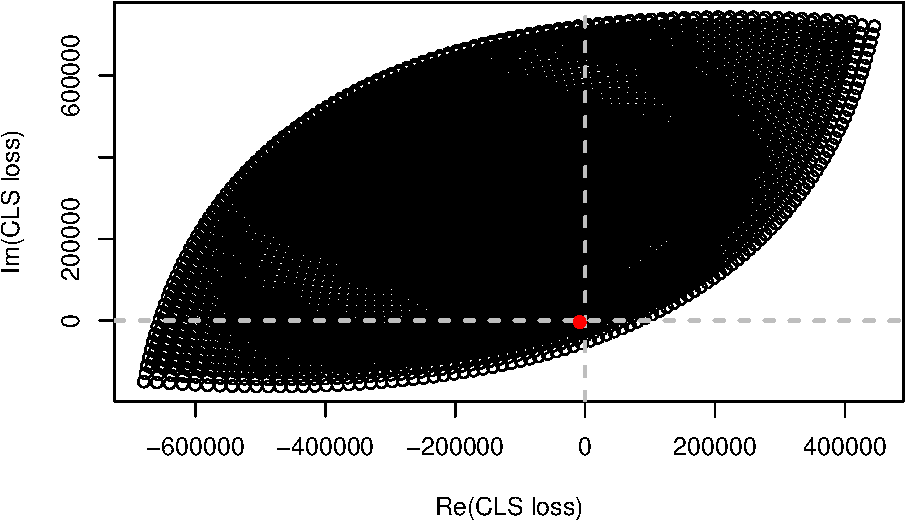
\includegraphics{Svetunkov---Svetunkov---Complex-Dynamic-Models_files/figure-latex/clsScatter-1.pdf}
\caption{\label{fig:clsScatter}Variety of CLS loss function values for different values of \(\underline{b_1}\).}
\end{figure}

Figure \ref{fig:clsScatter} shows a scatterplot of values of the complex loss \eqref{eq:SimpleCLRCLSLoss}. The red point close to the origin corresponds to the estimate obtained using \eqref{eq:SimpleCLRCLSLossParametersMoments}. As we can see, it is close to the origin, which implies that the minimisation of the loss \eqref{eq:SimpleCLRCLSLoss} is equivalent to making both real and imaginary parts of it close to zero. This means that CLS makes variances of real and imaginary residuals similar and shrinks the covariance between them to zero.

Another way of looking at how CLS works is to reduce its dimensionality via the Multidimensional Scaling \citep{Gower} and then visualise it. The R code below is relatively slow but produces a solution for this task.

\begin{Shaded}
\begin{Highlighting}[]
\CommentTok{\# Calculate distance matrix for all losses}
\CommentTok{\# (including the CLS point)}
\NormalTok{clsMDSDistance }\OtherTok{\textless{}{-}} \FunctionTok{dist}\NormalTok{(}\FunctionTok{rbind}\NormalTok{(clsValues[,}\DecValTok{3}\SpecialCharTok{:}\DecValTok{4}\NormalTok{],}
                             \FunctionTok{c}\NormalTok{(}\FunctionTok{Re}\NormalTok{(clsResult),}\FunctionTok{Im}\NormalTok{(clsResult))))}

\CommentTok{\# Do Multidimensional scaling}
\NormalTok{clsMDS }\OtherTok{\textless{}{-}} \FunctionTok{cmdscale}\NormalTok{(clsMDSDistance, }\AttributeTok{k=}\DecValTok{1}\NormalTok{)}

\CommentTok{\# Create a data frame with the coordinates}
\NormalTok{clsMDSValues }\OtherTok{\textless{}{-}} \FunctionTok{data.frame}\NormalTok{(}\AttributeTok{z=}\NormalTok{clsMDS,}
                           \AttributeTok{x=}\FunctionTok{c}\NormalTok{(clsValues[,}\DecValTok{1}\NormalTok{],}\FunctionTok{Re}\NormalTok{(bOptimal)),}
                           \AttributeTok{y=}\FunctionTok{c}\NormalTok{(clsValues[,}\DecValTok{2}\NormalTok{],}\FunctionTok{Im}\NormalTok{(bOptimal)))}

\CommentTok{\# Create a matrix with loss values for 3d plotting}
\NormalTok{clsMDSValuesZ }\OtherTok{\textless{}{-}} \FunctionTok{matrix}\NormalTok{(clsMDSValues}\SpecialCharTok{$}\NormalTok{z[}\SpecialCharTok{{-}}\DecValTok{10001}\NormalTok{], }\DecValTok{100}\NormalTok{, }\DecValTok{100}\NormalTok{)}
\end{Highlighting}
\end{Shaded}

Then, to produce the 3d surface on the plane of ``loss - \(b_{1,r}\) - \(b_{1,i}\), we can use functions from the \texttt{plotly} package in R as shown in the code below:

\begin{Shaded}
\begin{Highlighting}[]
\FunctionTok{plot\_ly}\NormalTok{(}\AttributeTok{z=}\NormalTok{clsMDSValuesZ,}
        \AttributeTok{x=}\FunctionTok{unique}\NormalTok{(clsMDSValues}\SpecialCharTok{$}\NormalTok{x[}\SpecialCharTok{{-}}\DecValTok{10001}\NormalTok{]),}
        \AttributeTok{y=}\FunctionTok{unique}\NormalTok{(clsMDSValues}\SpecialCharTok{$}\NormalTok{y[}\SpecialCharTok{{-}}\DecValTok{10001}\NormalTok{])) }\SpecialCharTok{|\textgreater{}}
\NormalTok{    plotly}\SpecialCharTok{::}\FunctionTok{layout}\NormalTok{(}\AttributeTok{scene=}\FunctionTok{list}\NormalTok{(}\AttributeTok{xaxis =} \FunctionTok{list}\NormalTok{(}\AttributeTok{title =} \StringTok{"Re(b1)"}\NormalTok{),}
                      \AttributeTok{yaxis =} \FunctionTok{list}\NormalTok{(}\AttributeTok{title =} \StringTok{"Im(b1)"}\NormalTok{),}
                      \AttributeTok{zaxis =} \FunctionTok{list}\NormalTok{(}\AttributeTok{title =} \StringTok{"MDS of CLS loss"}\NormalTok{))) }\SpecialCharTok{|\textgreater{}}
    \FunctionTok{add\_surface}\NormalTok{() }\SpecialCharTok{|\textgreater{}}
    \FunctionTok{add\_trace}\NormalTok{(}\AttributeTok{data =} \FunctionTok{tail}\NormalTok{(clsMDSValues,}\DecValTok{1}\NormalTok{),}
              \AttributeTok{x =} \SpecialCharTok{\textasciitilde{}}\NormalTok{x,}
              \AttributeTok{y =} \SpecialCharTok{\textasciitilde{}}\NormalTok{y,}
              \AttributeTok{z =} \SpecialCharTok{\textasciitilde{}}\NormalTok{z,}
              \AttributeTok{mode =} \StringTok{"markers"}\NormalTok{,}
              \AttributeTok{type =} \StringTok{"scatter3d"}\NormalTok{,}
              \AttributeTok{marker =} \FunctionTok{list}\NormalTok{(}\AttributeTok{size =} \DecValTok{10}\NormalTok{))}
\end{Highlighting}
\end{Shaded}

\begin{figure}
\centering
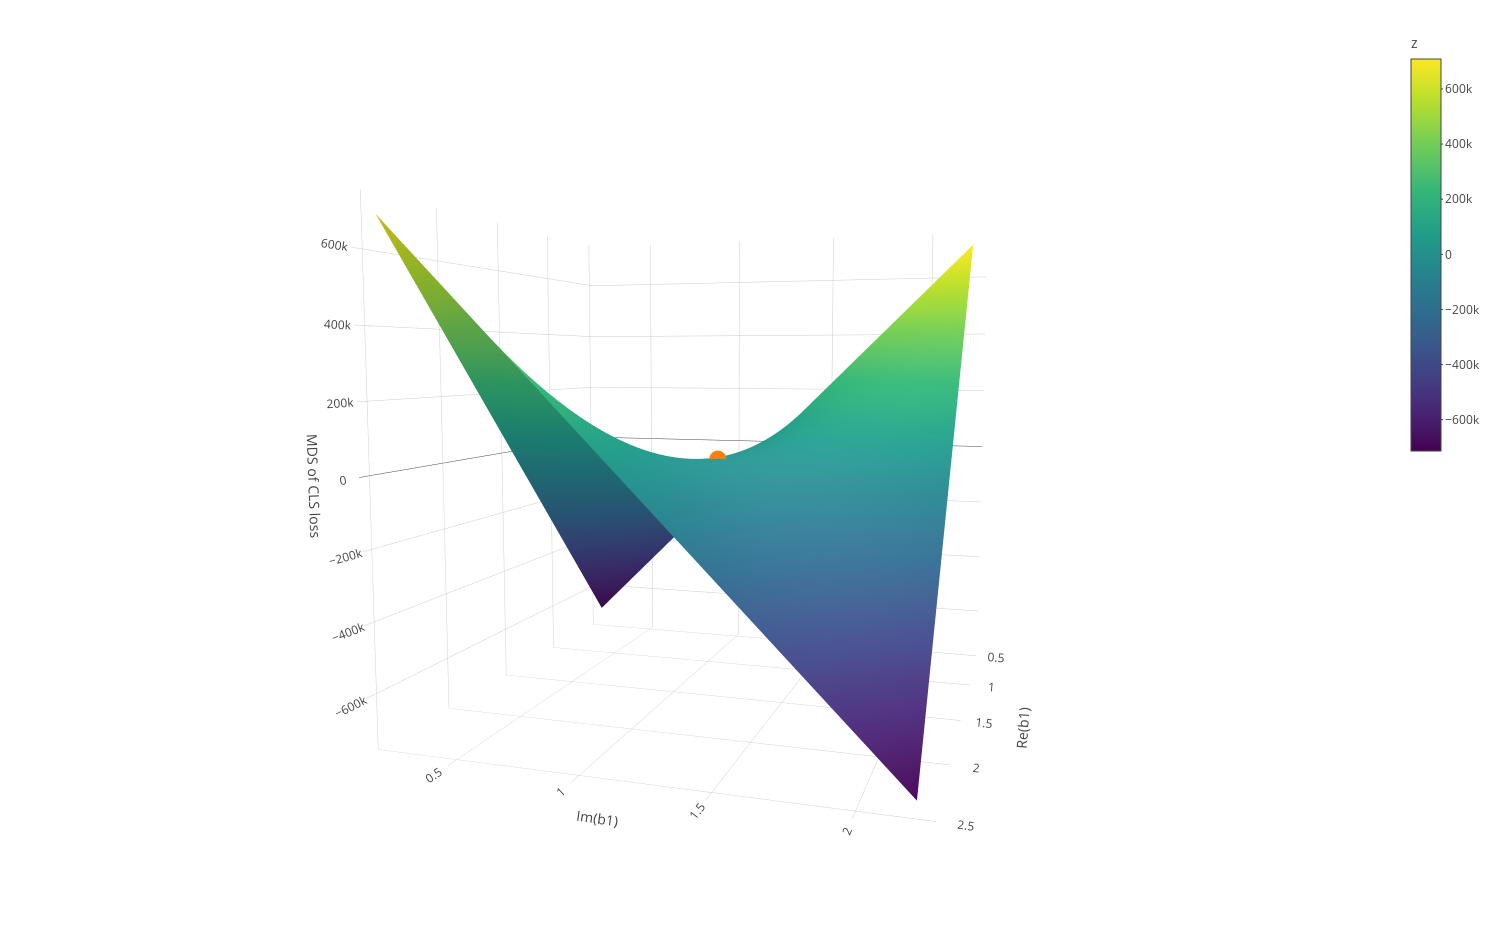
\includegraphics{images/CLSPlot.png}
\caption{\label{fig:plotlyCLS}Plot of the 3d surface for the MDS of the CLS loss.}
\end{figure}

Figure \ref{fig:plotlyCLS} demonstrates how the projection of the two-dimensional loss behaves for a variety of parameters of the regression. The orange point in the middle corresponds to the one obtained via CLS. We can see that it corresponds to the loss being close to zero, and represents a 2-dimensional inflection point, where the surface bends in different directions.

So, we can see that despite being counter-intuitive, the CLS produces the estimates of parameters that lead to the residuals being close to spherical (normal if we assume normality), because the variances of real and imaginary parts of the residuals become closer to each other, while the covariance between them becomes close to zero.

\hypertarget{SCLREstimationLikelihood}{%
\subsection{Likelihood}\label{SCLREstimationLikelihood}}

Finally, another way of estimating the simple CLR is by assuming a distribution of the residuals and maximising the respective likelihood. Given the connection between the linear and the vector forms of the complex regression, we can assume that the error term follows a multivariate normal distribution with a covariance matrix:
\begin{equation}
    \boldsymbol{\Sigma}_\epsilon = \begin{pmatrix} \sigma_{\epsilon_r}^2 & \sigma_{\epsilon_r, \epsilon_i} \\ \sigma_{\epsilon_r, \epsilon_i} & \sigma_{\epsilon_i}^2 \end{pmatrix} .
    \label{eq:SimpleCLRLikelihoodSigma}
\end{equation}
The log-likelihood in this case can be written as:
\begin{equation}
    \ell(\boldsymbol{\theta}, \boldsymbol{\Sigma}_\epsilon | \mathbf{Y}) = -\frac{n}{2} \left( 2 \log(2 \pi) + \log | \boldsymbol{\Sigma}_\epsilon| \right) -\frac{1}{2} \sum_{j=1}^n \left( \boldsymbol{\epsilon}_j^\prime \boldsymbol{\Sigma}_\epsilon^{-1} \boldsymbol{\epsilon}_j \right) ,
    \label{eq:additiveLogLik}
\end{equation}
where \(\boldsymbol{\theta}\) is the vector of estimated parameters and \(\boldsymbol{\epsilon}_j = \begin{pmatrix} \epsilon_{r,j} \\ \epsilon_{i,j} \end{pmatrix}\) is the two dimensional error term. This likelihood is maximised when the covariance matrix \eqref{eq:SimpleCLRLikelihoodSigma} is estimated via:
\begin{equation}
    \hat{\boldsymbol{\Sigma}}_\epsilon = \frac{1}{n} \sum_{j=1}^{n} \boldsymbol{e}_j \boldsymbol{e}_j^\prime .
    \label{eq:Sigmaest}
\end{equation}
It can be shown that if the \eqref{eq:Sigmaest} is inserted in \eqref{eq:additiveLogLik} then the following concentrated log-likelihood can be obtained \citep[see, for example,][]{Snyder2017}:
\begin{equation}
    \ell^*(\boldsymbol{\theta}, \hat{\boldsymbol{\Sigma}}_\epsilon | \mathbf{Y}) = -\frac{n}{2} \left( 2 \log(2 \pi e) + \log | \hat{\boldsymbol{\Sigma}}_\epsilon | \right) .
    \label{eq:additiveLogLikConcentrated}
\end{equation}
It is obvious that the maximisation of the log-likelihood \eqref{eq:additiveLogLikConcentrated} is equivalent to minimising the generalised variance of the complex error term (as discussed in Subsection \ref{crvSecondMoment}):
\begin{equation}
    \mathrm{GV} = |\hat{\boldsymbol{\Sigma}}_\epsilon| = \sigma_{\epsilon_r}^2 \sigma_{\epsilon_i}^2 - \sigma_{\epsilon_r, \epsilon_i}^2 .
    \label{eq:additiveLogLikConcentratedGV}
\end{equation}
The minimisation of GV in its turn implies the joint minimisation of variances of the real and imaginary part of the residuals and a maximisation of the square of the covariance between them, thus making the residuals more linearly related. This loss function might be especially useful if we indeed can assume that the real and imaginary part of the residuals are linearly related and we want to use this information in the estimation.

The main difference between the Likelihood and the other two estimators discussed in this Section is that the former can only be maximised via a numeric optimisation - there is no analytical solution for estimates of parameters via likelihood.

\hypertarget{SCLREstimatorsComparison}{%
\section{Comparing different estimators for SCLR}\label{SCLREstimatorsComparison}}

Arguably, all three estimators discussed in this Section give adequate estimates of parameters, but inevitably they will have different efficiency and would be appropriate in different situations. In this subsection, we will explore the performance of estimators with the increase of sample size.

First, comparing variances of OLS and CLS estimates of \(b_{1,r}\) \eqref{eq:SimpleCLRCLSb1Variance} with \eqref{eq:SimpleCLROLSb1Variance}:
\begin{equation*}
    \begin{aligned}
        \mathrm{V}(b_{1,r}^{\mathrm{OLS}}) = & \mathrm{V}\left(\frac{\hat{\sigma}_{x_r, \epsilon_r} + \hat{\sigma}_{x_i, \epsilon_i}}{\hat{\sigma}_{x_r}^2 + \hat{\sigma}_{x_i}^2}\right) \\
        \mathrm{V}(b_{1,r}^{\mathrm{CLS}}) = & \mathrm{V}\left(\frac{\left(\hat{\sigma}_{x_r, \epsilon_r} - \hat{\sigma}_{x_i, \epsilon_i}\right) \left(\hat{\sigma}_{x_r}^2 - \hat{\sigma}_{x_i}^2 \right) - 2 \hat{\sigma}_{x_r, x_i} \left(\hat{\sigma}_{x_r, \epsilon_i} + \hat{\sigma}_{x_i, \epsilon_r}\right)}{\left(\hat{\sigma}_{x_r}^2 - \hat{\sigma}_{x_i}^2\right)^2 + 4 \hat{\sigma}_{x_r, x_i}^2}\right)
    \end{aligned}
\end{equation*}
we can conclude that there are some situations, when the estimates of parameters via CLS are less efficient than the estimates via OLS. There are some cases, when the variance \eqref{eq:SimpleCLRCLSb1Variance} is much higher than \eqref{eq:SimpleCLROLSb1Variance}. For example, when the real and imaginary parts of \(x\) are not correlated (i.e.~\(\hat{\sigma}_{x_r, x_i}=0\)) and when the variances of the real and imaginary parts of \(x\) are equal, the variance of \(b_{1,r}\) explodes. However, there are also some cases, when CLS estimates are more efficient than the OLS ones. For example, when \(\hat{\sigma}_{x_r, \epsilon_i}=\hat{\sigma}_{x_i, \epsilon_i}\) and \(\hat{\sigma}_{x_r, x_i}=0\), the variance \eqref{eq:SimpleCLROLSb1Variance} will be equal to zero, while the variance \eqref{eq:SimpleCLRCLSb1Variance} will be greater than zero. So, in general, we cannot conclude which of the estimators will be more efficient, but we know that in different circumstances, they will have different properties.

We cannot compare the efficiency of the likelihood estimator directly with the OLS and CLS, but we know from the statistics literature \citep{referenceLikelihoodPaper} that likelihood gives consistent and asymptotically efficient estimates of parameters.

In terms of consistency, in one specific situation, when \(\hat{\sigma}_{x_r}^2 = \hat{\sigma}_{x_i}^2\) and \(\hat{\sigma}_{x_r, x_i}=0\), CLS might produce non-consistent estimates of parameters. This means that if we deal with explanatory variables with these properties, we should use either OLS or Likelihood.

Similar analysis can be done for the coefficient \(b_{1,i}\), with the conclusions similar to the above, so we skip this discussion.

In order to do a more thorough comparison of the three estimators, we set up an experiment based on the following simple CLR:
\begin{equation*}
    y_r + i y_i = 10+15i + (2-1.5i) (x_r + i x_i) + (\epsilon_r + i \epsilon_i)
\end{equation*}
with several scenarios, parameters for which are shown in Table \ref{tab:scenariosEstimators}. They covered several important situations: when \(x_r\) and \(x_i\) are not correlated, have medium correlation and perfectly correlated, when their variances are similar or different and then when the real and imaginary parts of the error term are not correlated, have medium correlation, are equal to zero and when their variances have high or low values.

\begin{table}

\caption{\label{tab:scenariosEstimators}Several scenarios for the comparison of estimators.}
\centering
\resizebox{\linewidth}{!}{
\fontsize{12}{14}\selectfont
\begin{tabular}[t]{l|l|l|l|l}
\hline
  & cor($x_r$, $x_i$) & std.dev. of $x_r$ and $x_i$ & cor($\epsilon_r$, $\epsilon_i$) & std.dev. of $\epsilon_r$ and $\epsilon_i$\\
\hline
Scenario 1 & 0 & $\sigma_{x_r}=10$, $\sigma_{x_i}=20$ & 0 & $\sigma_{\epsilon_r}=\sigma_{\epsilon_i}=1.5$\\
\hline
Scenario 2 & 1 & $\sigma_{x_r}=10$, while $\sigma_{x_i}=15$ & 0 & $\sigma_{\epsilon_r}=\sigma_{\epsilon_i}=1.5$\\
\hline
Scenario 3 & 0 & $\sigma_{x_r}=\sigma_{x_i}=20$ & 0 & $\sigma_{\epsilon_r}=\sigma_{\epsilon_i}=1.5$\\
\hline
Scenario 4 & medium & $\sigma_{x_r}=10$, $\sigma_{x_i}=15$ & NA & $\sigma_{\epsilon_r}=\sigma_{\epsilon_i}=0$\\
\hline
Scenario 5 & medium & $\sigma_{x_r}=10$, $\sigma_{x_i}=15$ & medium & $\sigma_{\epsilon_r}=10$, $\sigma_{\epsilon_i}=8$\\
\hline
Scenario 6 & medium & $\sigma_{x_r}=10$, $\sigma_{x_i}=15$ & 0 & $\sigma_{\epsilon_r}=\sigma_{\epsilon_i}=100$\\
\hline
\end{tabular}}
\end{table}

These six scenarios in Table \ref{tab:scenariosEstimators} cover different theoretically possible situations and show how the three estimators behave in these conditions. The sample size was first set to 20 observations and then was increased iteratively by one observation until reaching 10,000. This should give us an understanding of how the estimators behave both on small samples and asymptotically. While we recorded both values of estimated intercept and slope, we are mainly interested in the latter, and the plots shown below focus on how the complex \(\underline{b_1}\) is estimated. The experiments were done using \texttt{clm()} function from the \texttt{complex} package with \texttt{method} parameter equal to ``OLS'', ``CLS'' and ``likelihood'' for each of the respective estimators. A sample of the script used in the experiments is shown below:

\begin{Shaded}
\begin{Highlighting}[]
\NormalTok{obs }\OtherTok{\textless{}{-}} \DecValTok{10000}
\NormalTok{x0 }\OtherTok{\textless{}{-}} \FunctionTok{rnorm}\NormalTok{(obs,}\DecValTok{10}\NormalTok{,}\DecValTok{10}\NormalTok{)}
\NormalTok{x }\OtherTok{\textless{}{-}} \FunctionTok{complex}\NormalTok{(}\AttributeTok{real=}\NormalTok{x0,}\AttributeTok{imaginary=}\FunctionTok{rnorm}\NormalTok{(obs,}\DecValTok{0}\NormalTok{,}\DecValTok{10}\NormalTok{))}

\NormalTok{b0 }\OtherTok{\textless{}{-}} \DecValTok{10} \SpecialCharTok{+}\NormalTok{ 15i}
\NormalTok{b1 }\OtherTok{\textless{}{-}} \DecValTok{2}\FloatTok{{-}1.5}\NormalTok{i}
\NormalTok{y }\OtherTok{\textless{}{-}}\NormalTok{ b0 }\SpecialCharTok{+}\NormalTok{ b1 }\SpecialCharTok{*}\NormalTok{ x }\SpecialCharTok{+} \FloatTok{1.5}\SpecialCharTok{*}\FunctionTok{complex}\NormalTok{(}\AttributeTok{real=}\FunctionTok{rnorm}\NormalTok{(obs,}\DecValTok{0}\NormalTok{,}\DecValTok{1}\NormalTok{),}
                               \AttributeTok{imaginary=}\FunctionTok{rnorm}\NormalTok{(obs,}\DecValTok{0}\NormalTok{,}\DecValTok{1}\NormalTok{))}

\NormalTok{complexData }\OtherTok{\textless{}{-}} \FunctionTok{cbind}\NormalTok{(y,x)}

\NormalTok{nsim }\OtherTok{\textless{}{-}} \DecValTok{9980}
\NormalTok{parametersValues }\OtherTok{\textless{}{-}}
    \FunctionTok{array}\NormalTok{(}\ConstantTok{NA}\NormalTok{, }\FunctionTok{c}\NormalTok{(nsim,}\DecValTok{3}\NormalTok{,}\DecValTok{2}\NormalTok{),}
          \AttributeTok{dimnames=}\FunctionTok{list}\NormalTok{(}\ConstantTok{NULL}\NormalTok{,}
                        \FunctionTok{c}\NormalTok{(}\StringTok{"CLS"}\NormalTok{,}\StringTok{"OLS"}\NormalTok{,}\StringTok{"Likelihood"}\NormalTok{),}
                        \FunctionTok{c}\NormalTok{(}\StringTok{"b0"}\NormalTok{,}\StringTok{"b1"}\NormalTok{)))}

\ControlFlowTok{for}\NormalTok{(i }\ControlFlowTok{in} \DecValTok{1}\SpecialCharTok{:}\NormalTok{nsim)\{}
\NormalTok{    test }\OtherTok{\textless{}{-}} \FunctionTok{clm}\NormalTok{(y}\SpecialCharTok{\textasciitilde{}}\NormalTok{x, complexData, }\AttributeTok{loss=}\StringTok{"CLS"}\NormalTok{,}
                \AttributeTok{subset=}\FunctionTok{sample}\NormalTok{(}\FunctionTok{c}\NormalTok{(}\DecValTok{1}\SpecialCharTok{:}\NormalTok{obs),}\DecValTok{20}\SpecialCharTok{+}\NormalTok{i))}
\NormalTok{    parametersValues[i,}\DecValTok{1}\NormalTok{,] }\OtherTok{\textless{}{-}} \FunctionTok{coef}\NormalTok{(test)}
\NormalTok{    test }\OtherTok{\textless{}{-}} \FunctionTok{clm}\NormalTok{(y}\SpecialCharTok{\textasciitilde{}}\NormalTok{x, complexData, }\AttributeTok{loss=}\StringTok{"OLS"}\NormalTok{,}
                \AttributeTok{subset=}\FunctionTok{sample}\NormalTok{(}\FunctionTok{c}\NormalTok{(}\DecValTok{1}\SpecialCharTok{:}\NormalTok{obs),}\DecValTok{20}\SpecialCharTok{+}\NormalTok{i))}
\NormalTok{    parametersValues[i,}\DecValTok{2}\NormalTok{,] }\OtherTok{\textless{}{-}} \FunctionTok{coef}\NormalTok{(test)}
\NormalTok{    test }\OtherTok{\textless{}{-}} \FunctionTok{clm}\NormalTok{(y}\SpecialCharTok{\textasciitilde{}}\NormalTok{x, complexData, }\AttributeTok{loss=}\StringTok{"likelihood"}\NormalTok{,}
                \AttributeTok{subset=}\FunctionTok{sample}\NormalTok{(}\FunctionTok{c}\NormalTok{(}\DecValTok{1}\SpecialCharTok{:}\NormalTok{obs),}\DecValTok{20}\SpecialCharTok{+}\NormalTok{i))}
\NormalTok{    parametersValues[i,}\DecValTok{3}\NormalTok{,] }\OtherTok{\textless{}{-}} \FunctionTok{coef}\NormalTok{(test)}
\NormalTok{\}}
\end{Highlighting}
\end{Shaded}

Figure \ref{fig:parametersUCDV} demonstrates how estimates of parameters change with the increase of sample size in Scenario 1.

\begin{figure}
\centering
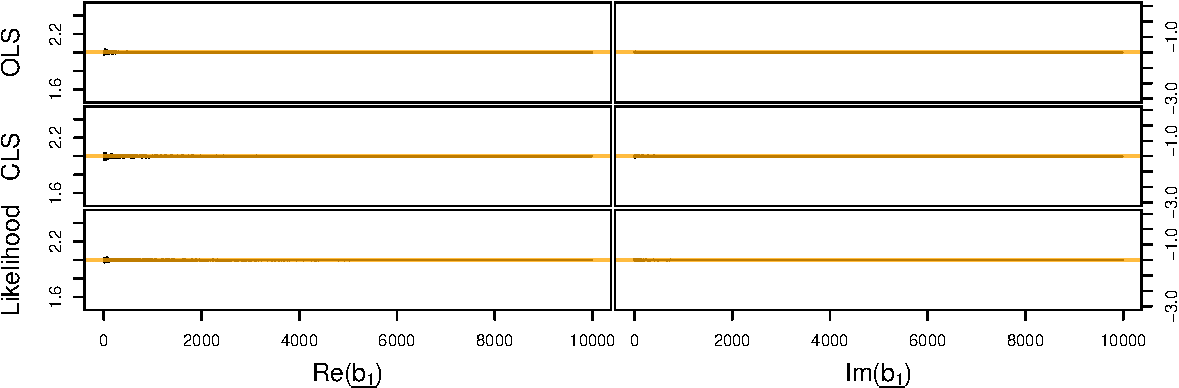
\includegraphics{Svetunkov---Svetunkov---Complex-Dynamic-Models_files/figure-latex/parametersUCDV-1.pdf}
\caption{\label{fig:parametersUCDV}Estimation of parameters using OLS, CLS and likelihood and their convergence to the true value of \(\underline{\beta_1}=2-1.5i\) (orange horizontal lines on the plot). Scenario 1.}
\end{figure}

Apparently, all three estimators produce very similar estimates of parameters in this case and converge to the true values quite fast. A similar behaviour is observed for the Scenario 2, shown in Figure \ref{fig:parametersPC}. The difference between the three estimators does not look substantial.

\begin{figure}
\centering
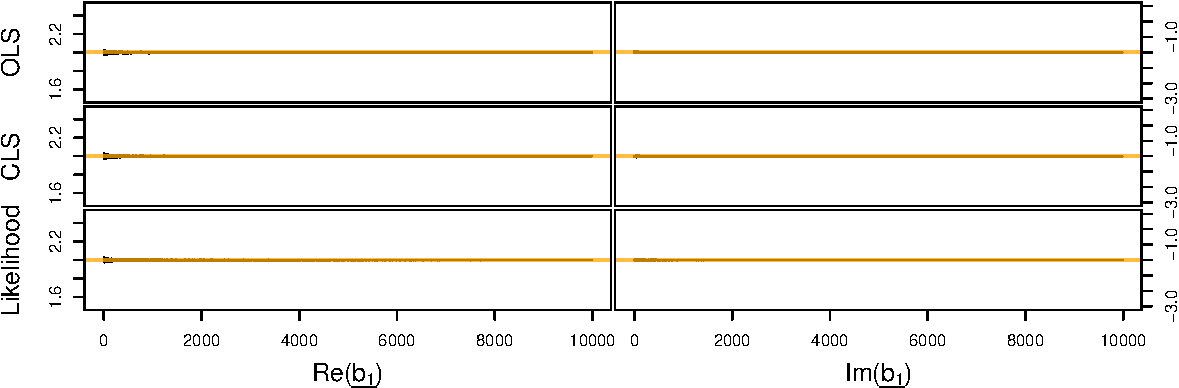
\includegraphics{Svetunkov---Svetunkov---Complex-Dynamic-Models_files/figure-latex/parametersPC-1.pdf}
\caption{\label{fig:parametersPC}Estimation of parameters using OLS, CLS and likelihood and their convergence to the true value of \(\underline{\beta_1}=2-1.5i\) (orange horizontal lines on the plot). Scenario 2.}
\end{figure}

In both Scenarios 1 and 2 the error term has a small variance, in Scenario 2 \(x_r\) and \(x_i\) are perfectly correlated, transforming the original model into: \(y_r + i y_i = 10+15i + (2-1.5i) (1 + 1.5 i) x_r + (\epsilon_r + i \epsilon_i)\).

The Scenario 3 demonstrates an exotic case, when the variances of \(x_r\) and \(x_i\) are the same (as shown in Figure \ref{fig:parametersUCSV}).

\begin{figure}
\centering
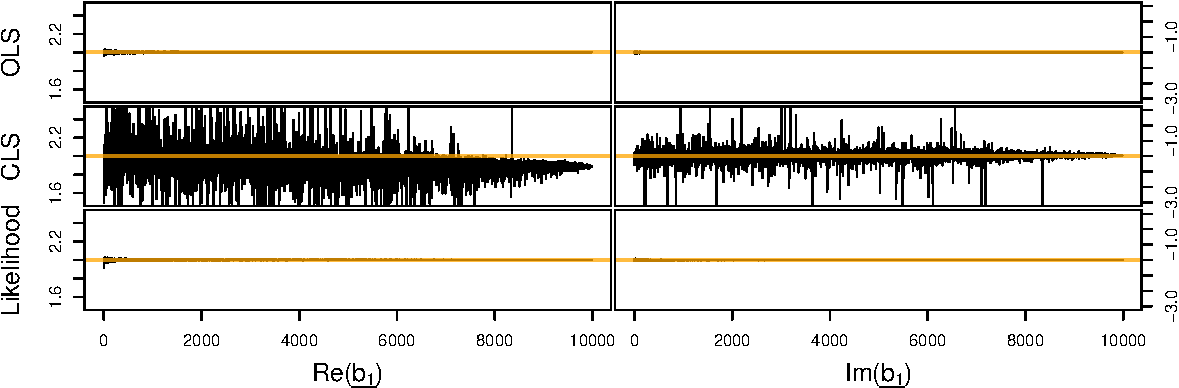
\includegraphics{Svetunkov---Svetunkov---Complex-Dynamic-Models_files/figure-latex/parametersUCSV-1.pdf}
\caption{\label{fig:parametersUCSV}Estimation of parameters using OLS, CLS and likelihood and their convergence to the true value of \(\underline{\beta_1}=2-1.5i\) (orange horizontal lines on the plot). Scenario 3.}
\end{figure}

In this scenario, OLS and Likelihood produce efficient, unbiased and consistent estimates of parameters, which cannot be said about the CLS. The behaviour of CLS is explainable because for this specific scenario the direct variance of the complex variable \(x_r + i x_i\) becomes close to zero. As a result, the direct covariance in \eqref{eq:SimpleCLRCLSLossParametersMomentsExpanded} is divided by zero, and the estimate of the parameter becomes unstable. Scenarios 1 and 3 could be considered as two special cases of the spectrum of values, showing that the closer the variances of the real and imaginary parts of \(x\) are, the less consistent, efficient and unbiased estimates of parameters are produced by CLS. Scenario 2 is complimentary, because it shows that if the real and imaginary parts are correlated, the CLS estimates of parameters become as good (in statistical terms) as the estimates of OLS and/or Likelihood. So, the CLS becomes unreliable in a special case, when \(\sigma_{x_r}^2 = \sigma_{x_i}^2\) and \(\sigma_{x_r,x_i}=0\).

Next, the three estimators give the same estimates of parameters in Scenario 4 of functional relation between \(x\) and \(y\), which is shown in Figure \ref{fig:parametersFR}.

\begin{figure}
\centering
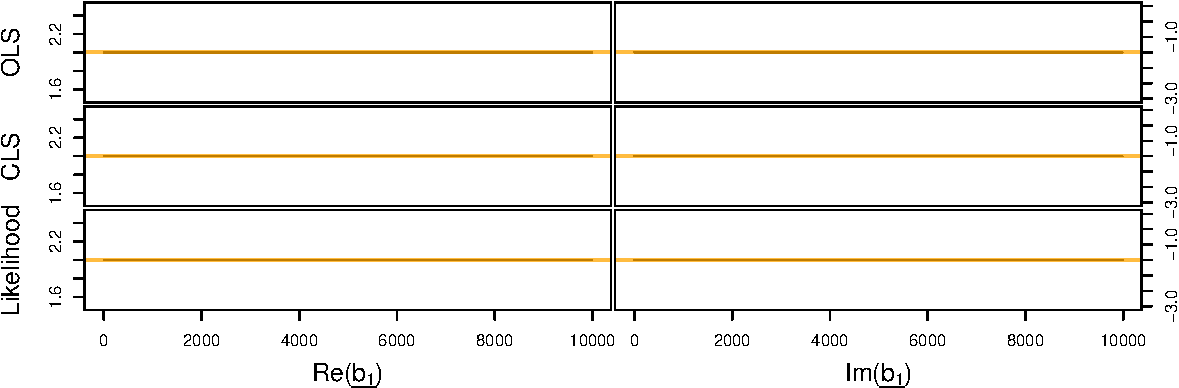
\includegraphics{Svetunkov---Svetunkov---Complex-Dynamic-Models_files/figure-latex/parametersFR-1.pdf}
\caption{\label{fig:parametersFR}Estimation of parameters using OLS, CLS and likelihood and their convergence to the true value of \(\underline{\beta_1}=2-1.5i\) (orange horizontal lines on the plot). Scenario 4.}
\end{figure}

The main difficulties for the estimators appear, when the variance of the error term increases. Figure \ref{fig:parametersCorError} shows how the three perform in case of a higher variance of the error term in Scenario 5.

\begin{figure}
\centering
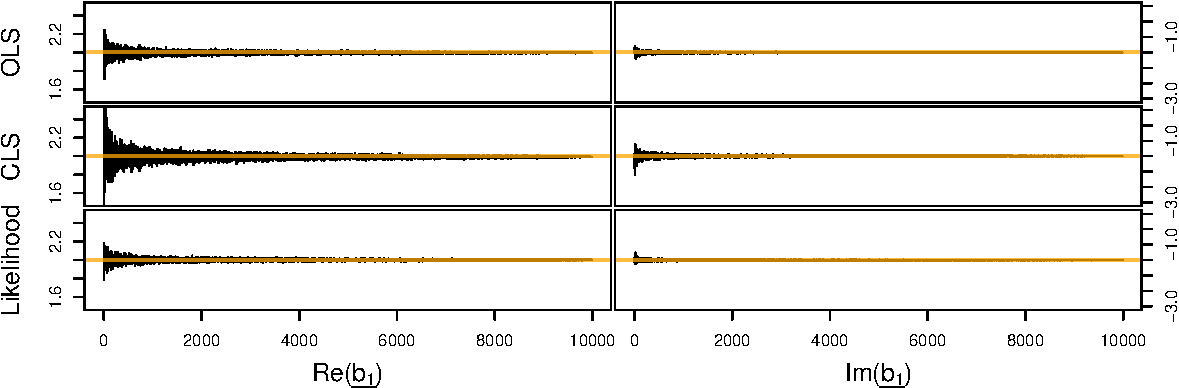
\includegraphics{Svetunkov---Svetunkov---Complex-Dynamic-Models_files/figure-latex/parametersCorError-1.pdf}
\caption{\label{fig:parametersCorError}Estimation of parameters using OLS, CLS and likelihood and their convergence to the true value of \(\underline{\beta_1}=2-1.5i\) (orange horizontal lines on the plot). Scenario 5.}
\end{figure}

It becomes apparent that OLS and Likelihood produce more efficient estimates of parameters than CLS on small samples. This is because the variability of estimates of parameter is higher for CLS than for the other two on small samples.

The situations worsens for the three estimators when we consider Scenario 6, when the variances of the error term become much higher than before, which is shown in Figure \ref{fig:parametersHVError}.

\begin{figure}
\centering
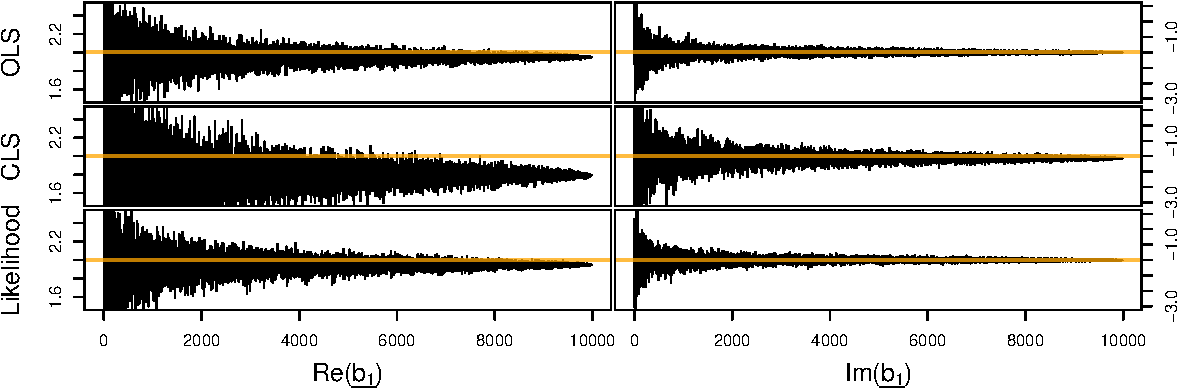
\includegraphics{Svetunkov---Svetunkov---Complex-Dynamic-Models_files/figure-latex/parametersHVError-1.pdf}
\caption{\label{fig:parametersHVError}Estimation of parameters using OLS, CLS and likelihood and their convergence to the true value of \(\underline{\beta_1}=2-1.5i\) (orange horizontal lines on the plot). Scenario 6.}
\end{figure}

In addition to being less efficient, the real parts of estimates of parameters exhibit a bias, which is diminished with the increase of sample size. Comparing the three estimators, it appears that CLS produces less efficient and more biased estimates of parameters than OLS or Likelihood in this Scenario.

These six scenarios show a variety of situations in which the three estimators produce different estimates of parameters. Arguably, OLS and Likelihood could be considered as robust alternatives, but all the three estimators seem to perform well in several sensible situations.

\hypertarget{correlationAnalysis}{%
\chapter{Correlation analysis of complex random variables}\label{correlationAnalysis}}

When it comes to measuring associations between variables, most frequently analysts use coefficient of correlation. While it is straightforward for real-valued variables, for complex variables this become challenging, because each c.r.v. has two parts, so the correlation needs to take them both into account.

For modelling purposes, it might be useful to have the information about all possible correlations involved relation of two c.r.v. This comes to analysing the following covariances for variables \(\underline{x}\) and \(\underline{y}\):

\begin{enumerate}
\def\labelenumi{\arabic{enumi}.}
\tightlist
\item
  \(\sigma_{x_r,x_i}\),
\item
  \(\sigma_{y_r,y_i}\),
\item
  \(\sigma_{x_r,y_r}\),
\item
  \(\sigma_{x_i,y_i}\),
\item
  \(\sigma_{x_r,y_i}\),
\item
  \(\sigma_{y_r,x_i}\).
\end{enumerate}

\hypertarget{correlationVisual}{%
\section{Visualisation of relations}\label{correlationVisual}}

In order to better understand what correlations between c.r.v. imply, we need to understand how to produce scatterplots for them. While in case of two real variables it is straightforward (a variable per axes), in our situation, this becomes challenging. We propose considering a set of scatterplots shown in Figure \ref{fig:crvScatterplots} for two generated complex random variables \(\underline{x}\) and \(\underline{y}\), created using \texttt{cplot()} function from \texttt{complex} package in R.

\begin{Shaded}
\begin{Highlighting}[]
\CommentTok{\# Create real part of a c.r.v. x}
\NormalTok{xr }\OtherTok{\textless{}{-}} \FunctionTok{rnorm}\NormalTok{(}\DecValTok{1000}\NormalTok{,}\DecValTok{0}\NormalTok{,}\DecValTok{10}\NormalTok{)}
\CommentTok{\# Create a c.r.v. x}
\NormalTok{x }\OtherTok{\textless{}{-}} \FunctionTok{complex}\NormalTok{(}\AttributeTok{real=}\NormalTok{xr, }\AttributeTok{imaginary=}\FloatTok{1.5}\SpecialCharTok{*}\NormalTok{xr}\SpecialCharTok{+}\FunctionTok{rnorm}\NormalTok{(}\DecValTok{1000}\NormalTok{,}\DecValTok{0}\NormalTok{,}\DecValTok{10}\NormalTok{))}
\CommentTok{\# Create a c.r.v. y}
\NormalTok{y }\OtherTok{\textless{}{-}}\NormalTok{ (}\DecValTok{10} \SpecialCharTok{+}\NormalTok{ 15i) }\SpecialCharTok{+}\NormalTok{ (}\FloatTok{1.5} \SpecialCharTok{+} \FloatTok{1.2}\NormalTok{i) }\SpecialCharTok{*}\NormalTok{ x }\SpecialCharTok{+}
    \FunctionTok{complex}\NormalTok{(}\AttributeTok{real=}\FunctionTok{rnorm}\NormalTok{(}\DecValTok{1000}\NormalTok{,}\DecValTok{0}\NormalTok{,}\DecValTok{10}\NormalTok{), }\AttributeTok{imaginary=}\FunctionTok{rnorm}\NormalTok{(}\DecValTok{1000}\NormalTok{,}\DecValTok{0}\NormalTok{,}\DecValTok{10}\NormalTok{))}
\CommentTok{\# Produce the plot}
\FunctionTok{cplot}\NormalTok{(x, y, }\AttributeTok{which=}\DecValTok{1}\NormalTok{)}
\end{Highlighting}
\end{Shaded}

\begin{figure}
\centering
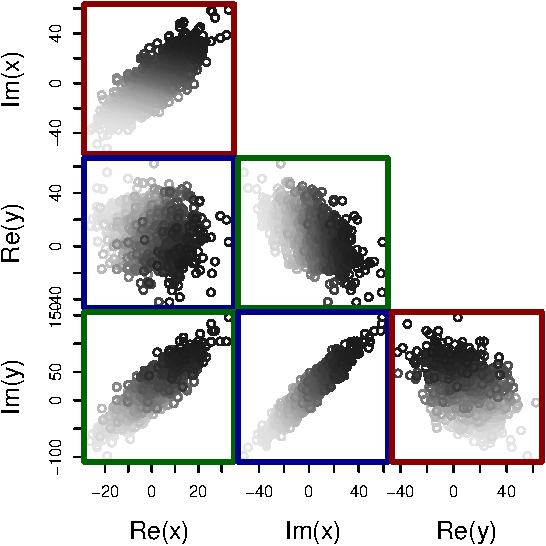
\includegraphics{Svetunkov---Svetunkov---Complex-Dynamic-Models_files/figure-latex/crvScatterplots-1.pdf}
\caption{\label{fig:crvScatterplots}Visualisation of relations between two complex variables}
\end{figure}

This scatterplot has several important elements in it:

\begin{itemize}
\tightlist
\item
  It shows relations between real and imaginary parts of each variable (e.g.~the two scatterplots in the bold dark red frame),
\item
  It shows cross-relations between parts of one variable and parts of the other one (e.g.~the rest four plots),
\item
  The colour shows ordering of the original variable \(\underline{x}\) with dark values corresponding to point with higher magnitude and light ones being closer to zero. This way, we can see what the original points in \(\underline{x}\) correspond to in \(\underline{y}\).
\end{itemize}

The plots are positioned to satisfy two rules:

\begin{enumerate}
\def\labelenumi{\arabic{enumi}.}
\tightlist
\item
  When a scatterplot for a c.r.v. is produced, the real part should be in x-axis, while the imaginary should be in the y-axis.
\item
  When parts of variables \(\underline{x}\) and \(\underline{y}\) are compared, the part for \(\underline{x}\) should be in x-axis, while the part for \(\underline{y}\) should be in y-axis, which should the reflect the idea that \(\underline{x}\) could be an explanatory variable for \(\underline{y}\).
\end{enumerate}

While a simple scatterplot matrix could have been constructed instead of Figure \ref{fig:crvScatterplots}, we argue that the latter has a logical grouping and should be preferred for analysis of complex variables. For example, based on the plots in Figure \ref{fig:crvScatterplots} we can conclude that:

\begin{itemize}
\tightlist
\item
  There is a positive relation between the real and imaginary parts of \(\underline{x}\),
\item
  There is a negative relation between the real and imaginary parts of \(\underline{y}\),
\item
  Real parts of \(\underline{x}\) and \(\underline{y}\) do not exhibit a strong linear relation,
\item
  But the respective imaginary parts of \(\underline{x}\) and \(\underline{y}\) have the positive relation between them,
\item
  Finally, we see that with the increase of real and imaginary parts of \(\underline{x}\), the real part of \(\underline{y}\) decreases, while the imaginary one increases. This sort of behaviour implies positive complex slope in the potential linear regression (discussed in Section \ref{simpleCLR}).
\end{itemize}

We think that this visualisation is useful when analysing relations between two complex random variables. But it also shows how complicated it is to capture the relation between them and how many aspects need to be considered.

As an alternative to the plot above, it is also possible to use some dimensionality reduction techniques to plot complex variables on a two dimensional plot. For example, we can use Multidimensional Scaling for this \citep[MDS,][]{refMDS} to create a project of one complex variable on x-axis and another one on the y-axis. In R, we can use the \texttt{cmdscale()} function from \texttt{stats} package for this (in the example below, we use euclidean distance for the dissimilarities matrix via \texttt{dist()} function from \texttt{stats}, and we use the \texttt{complex2vec()} function from \texttt{complex} package to transform complex variable to a collection of vectors):

\begin{Shaded}
\begin{Highlighting}[]
\NormalTok{xScaled }\OtherTok{\textless{}{-}} \FunctionTok{cmdscale}\NormalTok{(}\FunctionTok{dist}\NormalTok{(}\FunctionTok{complex2vec}\NormalTok{(x)), }\AttributeTok{k=}\DecValTok{1}\NormalTok{)}
\NormalTok{yScaled }\OtherTok{\textless{}{-}} \FunctionTok{cmdscale}\NormalTok{(}\FunctionTok{dist}\NormalTok{(}\FunctionTok{complex2vec}\NormalTok{(y)), }\AttributeTok{k=}\DecValTok{1}\NormalTok{)}
\FunctionTok{plot}\NormalTok{(xScaled,yScaled)}
\end{Highlighting}
\end{Shaded}

The same code is implemented in \texttt{cplot()} function from \texttt{complex} package in R:

\begin{Shaded}
\begin{Highlighting}[]
\FunctionTok{cplot}\NormalTok{(x, y, }\AttributeTok{which=}\DecValTok{2}\NormalTok{, }\AttributeTok{main=}\StringTok{""}\NormalTok{)}
\end{Highlighting}
\end{Shaded}

\begin{figure}
\centering
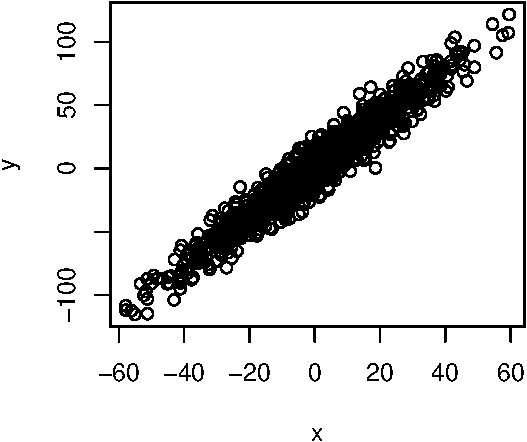
\includegraphics{Svetunkov---Svetunkov---Complex-Dynamic-Models_files/figure-latex/crvScatterplotMDS-1.pdf}
\caption{\label{fig:crvScatterplotMDS}Scatterplot of MDS of two complex variables.}
\end{figure}

The plot in Figure \ref{fig:crvScatterplotMDS} is much easier to read than the collection of scatterplots in Figure \ref{fig:crvScatterplots}, and in our example, we can conclude that the two complex variables exhibit strong linear relation.

\hypertarget{types-of-correlation-coefficients}{%
\section{Types of correlation coefficients}\label{types-of-correlation-coefficients}}

The literature knows two correlation coefficients for complex variables \citep{ref}: the conjugate and the direct correlation (the latter is known in the literature as ``pseudo-correlation''). Their formula are based on the respective covariances and variances (conjugate and direct discussed in Subsection \ref{crvSecondMoment}):

\begin{enumerate}
\def\labelenumi{\arabic{enumi}.}
\item
  Conjugate correlation
  \begin{equation}
   \rho_{x,y} = \frac{\sqrt{\sigma_{x,y} \sigma_{y,x}}}{\sigma_x \sigma_y},
   \label{eq:correlationConventional}
  \end{equation}
\item
  Direct correlation
  \begin{equation}
   \varrho_{x,y} = \frac{\varsigma_{x,y}}{\varsigma_x \varsigma_y}.
   \label{eq:correlationPseudo}
  \end{equation}
\end{enumerate}

Note that the conjugate correlation has the geometric mean of standard deviations in the numerator. This is needed because of the issue with the conjugate covariance (its value changes with the change of conjugate number). If we use only one of covariances \citep[as done, for example, by][]{Panchev1971} then the value of correlation coefficient will be ambiguous, implying that the correlation between \(\underline{x}\) and \(\underline{y}\) differs from the correlation between \(\underline{y}\) and \(\underline{x}\). Furthermore, such correlation coefficient would not work as intended. For example, if we have a positive functional linear relation between \(\underline{x}\) and \(\underline{y}\), the coefficient should be equal to one. But as an R example below demonstrates this value is obtained only if we have the geometric mean of covariances.

\begin{Shaded}
\begin{Highlighting}[]
\NormalTok{x }\OtherTok{\textless{}{-}} \FunctionTok{complex}\NormalTok{(}\AttributeTok{real=}\FunctionTok{rnorm}\NormalTok{(}\DecValTok{100}\NormalTok{,}\DecValTok{0}\NormalTok{,}\DecValTok{10}\NormalTok{), }\AttributeTok{imaginary=}\FunctionTok{rnorm}\NormalTok{(}\DecValTok{100}\NormalTok{,}\DecValTok{0}\NormalTok{,}\DecValTok{10}\NormalTok{))}
\NormalTok{y }\OtherTok{\textless{}{-}}\NormalTok{ (}\DecValTok{10} \SpecialCharTok{+}\NormalTok{ 15i) }\SpecialCharTok{+}\NormalTok{ (}\DecValTok{1} \SpecialCharTok{+}\NormalTok{ 1i) }\SpecialCharTok{*}\NormalTok{ x}
\CommentTok{\# Variant 1}
\FunctionTok{ccov}\NormalTok{(y,x,}\AttributeTok{method=}\StringTok{"conj"}\NormalTok{) }\SpecialCharTok{/}
    \FunctionTok{sqrt}\NormalTok{(}\FunctionTok{cvar}\NormalTok{(x,}\AttributeTok{method=}\StringTok{"conj"}\NormalTok{)}\SpecialCharTok{*}\FunctionTok{cvar}\NormalTok{(y,}\AttributeTok{method=}\StringTok{"conj"}\NormalTok{))}
\end{Highlighting}
\end{Shaded}

\begin{verbatim}
## [1] 0.7071068-0.7071068i
\end{verbatim}

\begin{Shaded}
\begin{Highlighting}[]
\CommentTok{\# Variant 2}
\FunctionTok{ccov}\NormalTok{(x,y,}\AttributeTok{method=}\StringTok{"conj"}\NormalTok{) }\SpecialCharTok{/}
    \FunctionTok{sqrt}\NormalTok{(}\FunctionTok{cvar}\NormalTok{(x,}\AttributeTok{method=}\StringTok{"conj"}\NormalTok{)}\SpecialCharTok{*}\FunctionTok{cvar}\NormalTok{(y,}\AttributeTok{method=}\StringTok{"conj"}\NormalTok{))}
\end{Highlighting}
\end{Shaded}

\begin{verbatim}
## [1] 0.7071068+0.7071068i
\end{verbatim}

\begin{Shaded}
\begin{Highlighting}[]
\CommentTok{\# Variant 3 (correct conjugate correlation)}
\FunctionTok{sqrt}\NormalTok{(}\FunctionTok{ccov}\NormalTok{(y,x,}\AttributeTok{method=}\StringTok{"conj"}\NormalTok{)}\SpecialCharTok{*}\FunctionTok{ccov}\NormalTok{(x,y,}\AttributeTok{method=}\StringTok{"conj"}\NormalTok{)) }\SpecialCharTok{/}
    \FunctionTok{sqrt}\NormalTok{((}\FunctionTok{cvar}\NormalTok{(x,}\AttributeTok{method=}\StringTok{"conj"}\NormalTok{)}\SpecialCharTok{*}\FunctionTok{cvar}\NormalTok{(y,}\AttributeTok{method=}\StringTok{"conj"}\NormalTok{)))}
\end{Highlighting}
\end{Shaded}

\begin{verbatim}
## [1] 1+0i
\end{verbatim}

The formulae \eqref{eq:correlationConventional} and \eqref{eq:correlationPseudo} are derived based on the original definition of Pearson's correlation coefficient \citep{refPearson}. It follows from the idea that the correlation coefficient equals to the geometric mean of slopes of two regression lines:
\begin{equation}
    \begin{aligned}
        &\underline{y} = \underline{\beta_0} + \underline{\beta_1} \underline{x} + \underline{\epsilon} \\
        &\underline{x} = \underline{\alpha_0} + \underline{\alpha_1} \underline{y} + \underline{\upsilon} ,
    \end{aligned}
    \label{eq:twoRegressions}
\end{equation}
where \(\underline{\alpha_0}\) and \(\underline{\beta_0}\) are the intercepts, \(\underline{\alpha_1}\) and \(\underline{\beta_1}\) are the slopes of the regression lines and \(\underline{\epsilon}\) and \(\underline{\upsilon}\) are the residuals of the models. Note that all of these variables and parameters in our case are complex. As discussed in Section \ref{simpleCLR}, the parameters of slope can be estimated using either Ordinary Least Squares, or the Complex Least Squares (discussed in Subsection \ref{SCLREstimation}). For the OLS, the formulae for the slopes are:
\begin{equation}
    \begin{aligned}
        &\underline{b_1} = \frac{\hat{\sigma}_{x,y}}{\hat{\sigma}_x} \\
        &\underline{a_1} = \frac{\hat{\sigma}_{y,x}}{\hat{\sigma}_y} .
    \end{aligned}
    \label{eq:twoRegressionsOLS}
\end{equation}
Taking their geometric means leads to:
\begin{equation}
    \hat{\rho}_{x,y} = \sqrt{\underline{a_1} \underline{b_1}},
    \label{eq:correlationConventionalEstimate}
\end{equation}
which then leads to the formula \eqref{eq:correlationConventional}. Similarly, for CLS estimated regressions, we have:
\begin{equation}
    \begin{aligned}
        &\underline{b_1} = \frac{\hat{\varsigma}_{x,y}}{\hat{\varsigma}_x} \\
        &\underline{a_1} = \frac{\hat{\varsigma}_{x,y}}{\hat{\varsigma}_y} ,
    \end{aligned}
    \label{eq:twoRegressionsCLS}
\end{equation}
which after taking the same geometric means leads to \eqref{eq:correlationPseudo}. Note that the estimates of the slope parameters will differ between the OLS and the CLS and thus the direct and conjugate correlations will differ as well.

\hypertarget{conjugate-correlation}{%
\section{Conjugate correlation}\label{conjugate-correlation}}

When it comes to the interpretation of the coefficients, the conjugate one is a real number. It can be written as:
\begin{equation}
    {\rho}_{x,y} = \frac{\sqrt{(\sigma_{x_r, y_r} + \sigma_{x_i, y_i})^2 + (\sigma_{x_i, y_r} - \sigma_{x_r, y_i})^2}}{\sqrt{(\sigma_{x_r}^2 + \sigma_{x_i}^2)(\sigma_{y_r}^2 + \sigma_{y_i}^2)}} .
    \label{eq:correlationConventionalExpanded}
\end{equation}
As can be seen from the formula \eqref{eq:correlationConventionalExpanded}, the coefficient is a real number, showing the average strength of linear relation between two complex variables \(\underline{x}\) and \(\underline{y}\). The coefficient will be equal to zero, when there are no linear relations between the respective real and imaginary parts of complex variables \(\underline{x}\) and \(\underline{y}\) and when the cross-covariances are equal (i.e.~\(\sigma_{x_r, y_r}=\sigma_{x_i, y_i}=0\) and \(\sigma_{x_i, y_r} = \sigma_{x_r, y_i}\)). A special case of this condition is when all the covariances are equal to zero. On the other hand, it will be close to one by absolute value if the complex relation between variables \(\underline{y}\) and \(\underline{x}\) is close to the linear, i.e.~\(\underline{a_1} = \frac{1}{\underline{b_1}}\).

In order to better understand what the conjugate correlation means, we expand the formula \eqref{eq:correlationConventionalEstimate} by substituting \(\underline{b_1} = b_{1,r} + i b_{1,i}\) and \(\underline{a_1} = a_{1,r} + i a_{1,i}\):
\begin{equation}
    \begin{aligned}
        \hat{\rho}_{x,y} = & \sqrt{(a_{1,r} + i a_{1,i}) (b_{1,r}+ib_{1,i})} = \\
        & \sqrt{a_{1,r} b_{1,r} - a_{1,i} b_{1,i} + i(a_{1,r} b_{1,i} + a_{1,i} b_{1,r})},
    \end{aligned}
    \label{eq:correlationConjugateExpanded01}
\end{equation}
or in the exponential form:
\begin{equation}
    \hat{\rho}_{x,y} = R^{\frac{1}{2}} e^{i \frac{1}{2} \phi} ,
    \label{eq:correlationConjugateExpanded02}
\end{equation}
where
\begin{equation}
    \begin{aligned}
        & R = \sqrt{(a_{1,r} b_{1,r} - a_{1,i} b_{1,i})^2 + (a_{1,r} b_{1,i} + a_{1,i} b_{1,r})^2} \\
        & \phi=\arctan\left(\frac{a_{1,r} b_{1,i} + a_{1,i} b_{1,r}}{a_{1,r} b_{1,r} - a_{1,i} b_{1,i}}\right),
    \end{aligned}
    \label{eq:correlationConjugateExpanded03}
\end{equation}
As can be seen from \eqref{eq:correlationConjugateExpanded03}, there is a multitude of combinations of parameters of the model that can give the unity magnitude \(R\). For example, if \(a_{1,r} = 0.5\), \(b_{1,r} = 1\), \(a_{1,i} = -0.5\) and \(b_{1,i} = 1\), \(R\) would be equal to one. Similarly, there is a multitude of values of parameters that would give angles of \(0\) and \(\pi\), leading to positive or negative real numbers. In fact, for the example above, \(\phi=0\), implying that the correlation coefficient will be equal to one, implying that the variables \(\underline{x}\) and \(\underline{y}\) exhibit a strong linear relation.

An R example of a conjugate correlation (via \texttt{ccor()} function from \texttt{complex} package) with the aforementioned values of parameters is shown below and in Figure \ref{fig:crvCorConjugate}.

\begin{Shaded}
\begin{Highlighting}[]
\CommentTok{\# Create a c.r.v. x}
\NormalTok{x }\OtherTok{\textless{}{-}} \FunctionTok{complex}\NormalTok{(}\AttributeTok{real=}\FunctionTok{rnorm}\NormalTok{(}\DecValTok{100}\NormalTok{,}\DecValTok{0}\NormalTok{,}\DecValTok{10}\NormalTok{), }\AttributeTok{imaginary=}\FunctionTok{rnorm}\NormalTok{(}\DecValTok{100}\NormalTok{,}\DecValTok{0}\NormalTok{,}\DecValTok{10}\NormalTok{))}
\CommentTok{\# Create a c.r.v. y}
\NormalTok{y }\OtherTok{\textless{}{-}}\NormalTok{ (}\DecValTok{10} \SpecialCharTok{+}\NormalTok{ 15i) }\SpecialCharTok{+}\NormalTok{ (}\DecValTok{1} \SpecialCharTok{+}\NormalTok{ 1i) }\SpecialCharTok{*}\NormalTok{ x }\SpecialCharTok{+}
    \FunctionTok{complex}\NormalTok{(}\AttributeTok{real=}\FunctionTok{rnorm}\NormalTok{(}\DecValTok{100}\NormalTok{,}\DecValTok{0}\NormalTok{,}\DecValTok{1}\NormalTok{), }\AttributeTok{imaginary=}\FunctionTok{rnorm}\NormalTok{(}\DecValTok{100}\NormalTok{,}\DecValTok{0}\NormalTok{,}\DecValTok{1}\NormalTok{))}
\CommentTok{\# Produce the plot}
\FunctionTok{cplot}\NormalTok{(x, y, }\AttributeTok{main=}\StringTok{""}\NormalTok{)}
\end{Highlighting}
\end{Shaded}

\begin{figure}
\centering
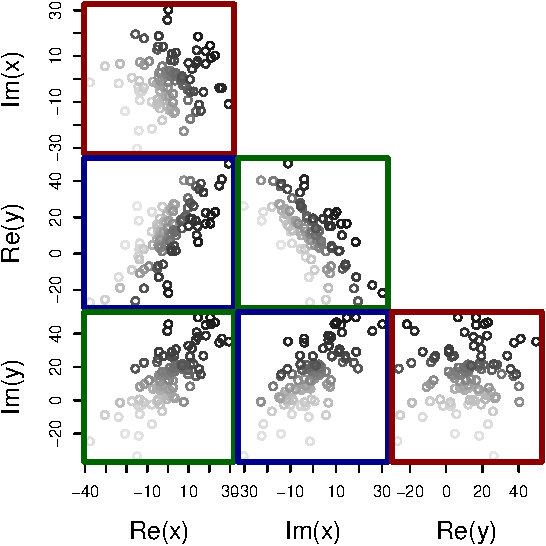
\includegraphics{Svetunkov---Svetunkov---Complex-Dynamic-Models_files/figure-latex/crvCorConjugate-1.pdf}
\caption{\label{fig:crvCorConjugate}Two complex variables with conjugate correlation being close to one.}
\end{figure}

\begin{Shaded}
\begin{Highlighting}[]
\CommentTok{\# Conjugate correlation}
\FunctionTok{ccor}\NormalTok{(x, y, }\AttributeTok{method=}\StringTok{"conjugate"}\NormalTok{)}
\end{Highlighting}
\end{Shaded}

\begin{verbatim}
## [1] 0.9981047+0i
\end{verbatim}

As can be seen from the Figure \ref{fig:crvCorConjugate} and the value of the conjugate correlation, there is a relation between the two complex variables \(\underline{x}\) and \(\underline{y}\). The conjugate correlation says that this is a strong linear relation, and one of ways how we can check this is by analysing the MDS of the two variables.

\begin{Shaded}
\begin{Highlighting}[]
\FunctionTok{cplot}\NormalTok{(x, y, }\AttributeTok{which=}\DecValTok{2}\NormalTok{, }\AttributeTok{main=}\StringTok{""}\NormalTok{)}
\end{Highlighting}
\end{Shaded}

\begin{figure}
\centering
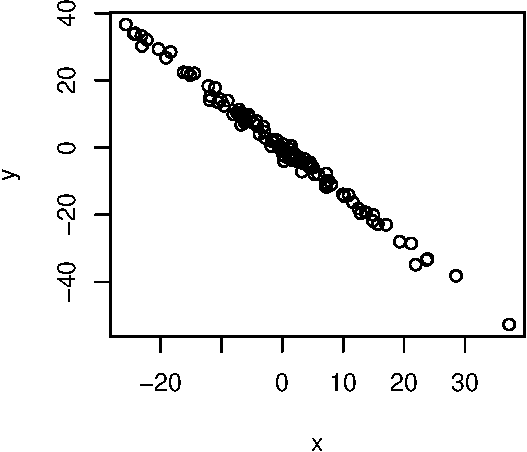
\includegraphics{Svetunkov---Svetunkov---Complex-Dynamic-Models_files/figure-latex/crvCorConjugateMDS-1.pdf}
\caption{\label{fig:crvCorConjugateMDS}Visualisation of relations between two complex variables}
\end{figure}

As can be seen from the plot in Figure \ref{fig:crvCorConjugateMDS}, it seems that the variables indeed exhibit a strong linear relation. So, the conjugate correlation has provided an adequate information about it.

\hypertarget{direct-correlation}{%
\section{Direct correlation}\label{direct-correlation}}

The direct correlation can be expanded to:
\begin{equation}
    {\varrho}_{x,y} = \frac{\sigma_{x_r, y_r} - \sigma_{x_i, y_i} + i (\sigma_{x_i, y_r} + \sigma_{x_r, y_i})}{\sqrt{(\sigma_{x_r}^2 - \sigma_{x_i}^2 + i2 \sigma_{x_r,x_i})(\sigma_{y_r}^2 - \sigma_{y_i}^2 + i2 \sigma_{y_r,y_i})}}.
    \label{eq:correlationPseudoExpanded}
\end{equation}
Given that it contains a complex number in the denominator, it is more complicated than the conjugate one. But it has several apparent properties:

\begin{enumerate}
\def\labelenumi{\arabic{enumi}.}
\item
  The magnitude of the coefficient will be equal to zero (and thus the coefficient will be equal to zero) only when \(\sigma_{x_i,y_r}=\sigma_{x_r,y_i}=0\) and \(\sigma_{x_r,y_r}=\sigma_{x_i,y_i}\). One of the special cases of this is when all cross-covariances between the real and imaginary parts of \(\underline{x}\) and \(\underline{y}\) are equal to zero.
\item
  When the complex variables \(\underline{x}\) and \(\underline{y}\) have functional relation between them, so that \(\underline{a_1} = \frac{1}{\underline{b_1}}\), the coefficient will be equal to one.
\end{enumerate}

Note however that due to the division by a complex number, the value of 1 can also be obtained due to the values of direct variance of variables \(\underline{x}\) and/or \(\underline{y}\).

Coefficient equal to -1 and to i.

\hypertarget{pearsons-correlation}{%
\section{Pearson's correlation}\label{pearsons-correlation}}

We can also use MDS to analyse the projections of complex variables on x and y axes, similar to how we have done that in Subsection \ref{correlationVisual}. In that case, we can calculate Pearson's correlation coefficient:

\begin{Shaded}
\begin{Highlighting}[]
\CommentTok{\# Create projections of two complex variables onto axes}
\NormalTok{xScaled }\OtherTok{\textless{}{-}} \FunctionTok{cmdscale}\NormalTok{(}\FunctionTok{dist}\NormalTok{(}\FunctionTok{complex2vec}\NormalTok{(x)), }\AttributeTok{k=}\DecValTok{1}\NormalTok{)}
\NormalTok{yScaled }\OtherTok{\textless{}{-}} \FunctionTok{cmdscale}\NormalTok{(}\FunctionTok{dist}\NormalTok{(}\FunctionTok{complex2vec}\NormalTok{(y)), }\AttributeTok{k=}\DecValTok{1}\NormalTok{)}
\CommentTok{\# Calculate the correlation coefficient}
\FunctionTok{cor}\NormalTok{(xScaled,yScaled)}
\end{Highlighting}
\end{Shaded}

\begin{verbatim}
##          [,1]
## [1,] 0.997496
\end{verbatim}

Or using the \texttt{ccor()} function with \texttt{method="pearson"}, which does exactly the same thing in one line of code:

\begin{Shaded}
\begin{Highlighting}[]
\FunctionTok{ccor}\NormalTok{(x, y, }\AttributeTok{method=}\StringTok{"pearson"}\NormalTok{)}
\end{Highlighting}
\end{Shaded}

The interpretation of the coefficient is straightforward and follows the conventional interpretation taught in any Statistics module. Note however that in general in the optimisation phase of MDS, it can reach the local optimum and not being able to get to the global one. As a result, the sign of the correlation might not represent the real relation between the two complex variables and in general should be ignored. Furthermore, inevitably when we move from four dimensions to two, we loose some information, so this approach is prone to possible mistakes and should be used with care. Finally, MDS is computationally expensive, especially on the long series. This means that in some cases it might take plenty of time before we get the Pearson's correlation value. Nonetheless, this is an additional way of analysing relations between complex variables.

\hypertarget{correlation-matrix}{%
\section{Correlation matrix}\label{correlation-matrix}}

Finally, as discussed in Subsection \ref{crvSecondMoment}, it is possible to calculate the covariance matrix between two c.r.v. Based on that matrix, we can calculate the correlation matrix, which will summarise all the relations between the real and imaginary parts of \(\underline{x}\) and \(\underline{y}\). This is done by dividing each element of the covariance matrix by geometric means of variances of the variables under consideration. In R, this can be done using \texttt{covar()} function from the \texttt{complex} package and \texttt{cov2cor()} function from the \texttt{stats} package:

\begin{Shaded}
\begin{Highlighting}[]
\FunctionTok{cov2cor}\NormalTok{(}\FunctionTok{covar}\NormalTok{(}\FunctionTok{cbind}\NormalTok{(x,y)))}
\end{Highlighting}
\end{Shaded}

\begin{verbatim}
##           x_r        x_i         y_r         y_i
## x_r 1.0000000  0.1166088  0.64563819  0.73476935
## x_i 0.1166088  1.0000000 -0.67970883  0.75751947
## y_r 0.6456382 -0.6797088  1.00000000 -0.03976467
## y_i 0.7347693  0.7575195 -0.03976467  1.00000000
\end{verbatim}

This matrix will not tell us how the variables \(\underline{x}\) and \(\underline{y}\) are related overall, but it will contain information about each of their individual elements.

\hypertarget{multipleCLR}{%
\chapter{Multiple Complex Linear Regression}\label{multipleCLR}}

We now move to the discussion of the multiple CLR, the model that captures relations between one complex random variable, \(y_r + i y_i\) and a set of explanatory complex random variables.

\hypertarget{model-formulation}{%
\section{Model formulation}\label{model-formulation}}

Similarly to how the multiple linear regression is formulated for real valued variables, the multiple complex linear regression can be written as:
\begin{equation}
    \underline{y_j} = \underline{\beta_0} + \underline{\beta_1} \underline{x_{1,j}} + \underline{\beta_2} \underline{x_{2,j}} + \dots + \underline{\beta_k} \underline{x_{k,j}} + \underline{\epsilon_j},
    \label{eq:MultipleCLRComplex}
\end{equation}
where \(k\) is the number of complex random variables. Similarly to how it was done with SCLR in \eqref{eq:SimpleCLRSystem}, we can expand the formula \eqref{eq:MultipleCLRComplex} as a system of two equations, taking that every parameter and every variable in \eqref{eq:MultipleCLRComplex} is complex:
\begin{equation}
    \begin{aligned}
        y_{r,j} = & \beta_{0,r} + \beta_{1,r} x_{1,r,j} - \beta_{1,i} x_{1,i,j} + \dots + \beta_{k,r} x_{k,r,j} - \beta_{k,i} x_{k,i,j} + \epsilon_{r,j} \\
        y_{i,j} = & \beta_{0,i} + \beta_{1,r} x_{1,i,j} + \beta_{1,i} x_{1,r,j} + \dots + \beta_{k,r} x_{k,i,j} + \beta_{k,i} x_{k,r,j} + \epsilon_{i,j} .
    \end{aligned}
    \label{eq:MultipleCLRSystem}
\end{equation}
As can be seen from \eqref{eq:MultipleCLRSystem}, the multiple CLR captures more complex dynamics than the conventional multiple linear regression. Both parts of the system use the same set of parameters and explanatory variables, but in different combinations, resulting in a versatile modelling framework.

This system can be represented in a more compact form, similarly to \eqref{eq:SimpleCLRVector}:
\begin{equation}
    \underline{\mathbf{y}} = \underline{\mathbf{X}} \underline{\boldsymbol{\beta}} + \underline{\boldsymbol{\epsilon}} ,
    \label{eq:CLRVector}
\end{equation}
where now \(\underline{\mathbf{X}} = \begin{pmatrix} 1 & \underline{{x}_{1,1}} & \dots & \underline{{x}_{k,1}} \\ 1 & \underline{{x}_{1,2}} & \dots & \underline{{x}_{k,2}} \\ \vdots & \vdots & \ddots & \vdots \\ 1 & \underline{{x}_{1,n}} & \dots & \underline{{x}_{k,n}} \end{pmatrix}\) and \(\underline{\boldsymbol{\beta}} = \begin{pmatrix} \underline{{\beta}_0} \\ \underline{{\beta}_1} \\ \vdots \\ \underline{{\beta}_k} \end{pmatrix}\), where each of the elements in the matrices and vectors above is a complex number.

Furthermore, the system \eqref{eq:MultipleCLRSystem} can also be used to represent the multiple CLR in a simple form using vector and matrix notations, avoiding complex numbers:
\begin{equation}
    \mathbf{y}_j = \underset{\sim}{\mathbf{X}_j} \boldsymbol{\beta} + \boldsymbol{\epsilon}_j ,
    \label{eq:MultipleCLRSystemVector}
\end{equation}
where \(\mathbf{y}_j = \begin{pmatrix} y_{r,j} \\ y_{i,j} \end{pmatrix}\), \(\underset{\sim}{\mathbf{X}_j} = \begin{pmatrix} 1 & 0 & x_{1,r,j} & -x_{1,i,j} & \dots & x_{k,r,j} & -x_{k,i,j} \\ 0 & 1 & x_{1,i,j} & x_{1,r,j} & \dots & x_{k,i,j} & x_{k,r,j} \end{pmatrix}\), \(\boldsymbol{\beta}^\prime = \begin{pmatrix} \beta_{0,r} & \beta_{0,i} & \beta_{1,r} & \beta_{1,i} & \dots & \beta_{1,k} & \beta_{1,k} \end{pmatrix}\) and \(\mathbf{\epsilon}_j = \begin{pmatrix} \epsilon_{r,j} \\ \epsilon_{i,j} \end{pmatrix}\). This can be then represented in the even more compact form, using the same principles as discussed in Section \ref{simpleCLRModel} in formula \eqref{eq:SimpleCLRSystemVectorFinal}:
\begin{equation}
    \mathbf{Y} = \underset{\sim}{\mathbf{X}} \boldsymbol{\beta} + \mathbf{E} 
    \label{eq:CLRSystemVectorFinal}
\end{equation}
with where \(\mathbf{Y}=\begin{pmatrix}\mathbf{y}_1 \\ \mathbf{y}_2\\ \vdots \\ \mathbf{y}_n \end{pmatrix}\), \(\underset{\sim}{\mathbf{X}}=\begin{pmatrix} \underset{\sim}{\mathbf{X}_1} \\ \underset{\sim}{\mathbf{X}_2} \\ \vdots \\ \underset{\sim}{\mathbf{X}_n} \end{pmatrix}\) and \(\mathbf{E}=\begin{pmatrix}\boldsymbol{\epsilon}_1 \\ \boldsymbol{\epsilon}_2\\ \vdots \\ \boldsymbol{\epsilon}_n \end{pmatrix}\). Formula \eqref{eq:CLRSystemVectorFinal} becomes especially useful for multiple CLR for the model estimation via OLS, CLS or Likelihood in the matrix form. The form \eqref{eq:CLRSystemVectorFinal} sidesteps complex numbers all together, representing the set of equations in matrices and vectors, containing real numbers only. This is convenient for many purposes and in inference.

The main difference between the form \eqref{eq:CLRVector} and \eqref{eq:CLRSystemVectorFinal} is that the former contains complex numbers inside each of the matrices and vectors.

\hypertarget{estimation}{%
\section{Estimation}\label{estimation}}

In order to estimate the parameters of the model \eqref{eq:CLRVector}, we can use the same methods as in the Chapter \ref{simpleCLR}: OLS, CLS and Likelihood. We will write the estimated model as:
\begin{equation}
    \underline{\mathbf{y}} = \underline{\mathbf{X}} \underline{\boldsymbol{b}} + \underline{\mathbf{e}} ,
    \label{eq:CLRVectorEstimated}
\end{equation}
where \(\underline{\boldsymbol{b}}\) is the estimate of \(\underline{\boldsymbol{\beta}}\) and \(\underline{\mathbf{e}}\) is the estimate of \(\underline{\mathbf{\epsilon}}\). And in case of matrix notations, instead of \eqref{eq:CLRSystemVectorFinal} we will have:
\begin{equation}
    \mathbf{Y} = \underset{\sim}{\mathbf{X}} \boldsymbol{b} + \mathbf{\hat{E}} 
    \label{eq:CLRSystemVectorFinalEstimated}
\end{equation}

\hypertarget{ordinary-least-squares-1}{%
\subsection{Ordinary Least Squares}\label{ordinary-least-squares-1}}

The criterion of OLS for multiple CLR can be written as:
\begin{equation}
    \min S^{\mathrm{OLS}}(\underline{\boldsymbol{b}}) = \min \left(\underline{\mathbf{e}}^\prime \underline{\mathbf{e}}\right),
    \label{eq:CLROLSCriterion}
\end{equation}
which can be expanded to:
\begin{equation}
    \begin{aligned}
    S^{\mathrm{OLS}}(\underline{\boldsymbol{b}}) = & \left( \underline{\mathbf{y}} - \underline{\mathbf{X}} \underline{\boldsymbol{b}} \right)^\prime \left( \underline{\mathbf{y}} - \underline{\mathbf{X}} \underline{\boldsymbol{b}} \right) = \\
    & \underline{\mathbf{y}}^\prime \underline{\mathbf{y}} - \underline{\mathbf{y}}^\prime \underline{\mathbf{X}} \underline{\boldsymbol{b}} - \underline{\boldsymbol{b}}^\prime \underline{\mathbf{X}}^\prime \underline{\mathbf{y}} + \underline{\boldsymbol{b}}^\prime \underline{\mathbf{X}}^\prime \underline{\mathbf{X}} \underline{\boldsymbol{b}}
    \end{aligned}. 
    \label{eq:CLROLSCriterionExpanded}
\end{equation}
Taking derivative of \eqref{eq:CLROLSCriterionExpanded} with respect to \(\underline{\boldsymbol{b}}\) and equating it to zero, results in the following system of normal equations:
\begin{equation}
    \underline{\mathbf{X}}^\prime \underline{\mathbf{X}} \underline{\boldsymbol{b}} = \underline{\mathbf{X}}^\prime \underline{\mathbf{y}} ,
    \label{eq:CLROLSSystemOfNormalEquations}
\end{equation}
which gives the classical formula for the estimation of parameters of the model \eqref{eq:CLRSystemVectorFinal}:
\begin{equation}
    \underline{\boldsymbol{b}} = \left( \underline{\mathbf{X}}^\prime \underline{\mathbf{X}} \right)^{-1} \underline{\mathbf{X}}^\prime \underline{\mathbf{y}}
    \label{eq:MCLROLSEstimate}
\end{equation}
Given that \eqref{eq:MCLROLSEstimate} corresponds to the classical OLS, it will maintain all of its conventional properties, i.e.~its estimates being unbiased, efficient and consistent. Note that, as discussed Subsection \ref{complexVariable}, the operator \(\prime\) denotes conjugate transposition, which means that for the special case of simple CLR, the formula \eqref{eq:MCLROLSEstimate} will become \eqref{eq:SimpleCLROLSLossParametersMoments}.

Finally, using the same principles, we can show that the estimates of parameters can be obtained if we use the form \eqref{eq:CLRSystemVectorFinalEstimated} instead of the vectors of complex variables:
\begin{equation}
    \boldsymbol{b} = \left( \underset{\sim}{\mathbf{\tilde{X}}}^\prime \underset{\sim}{\mathbf{X}}\right)^{-1} \underset{\sim}{\mathbf{\tilde{X}}}^\prime {\mathbf{Y}} .
    \label{eq:MCLROLSEstimateComplex}
\end{equation}
The form \eqref{eq:MCLROLSEstimateComplex} becomes especially useful for futher inference.

\hypertarget{complex-least-squares}{%
\subsection{Complex Least Squares}\label{complex-least-squares}}

As discussed in Section \ref{SCLREstimation}, there is also an alternative approach to estimation of CLR, the Complex Least Squares. In order to get the estimates based on it, we need to apply the same principles as with OLS, but directly to the form \eqref{eq:CLRVector}, i.e.~minimise the criterion (which is the same as the one discussed in Subsection \ref{SCLREstimationCLS}):
\begin{equation}
    \min S^{\mathrm{CLS}}(\underline{\boldsymbol{b}}) = \min \left(\underline{\mathbf{e}}^\top \underline{\mathbf{e}}\right).
    \label{eq:CLRCLSCriterion}
\end{equation}
Using the same logic as with OLS, it can be shown that the minimisation of this criterion implies the solution of the following system of normal equations:
\begin{equation}
    \underline{\mathbf{X}}^\top \underline{\mathbf{X}} \underline{\boldsymbol{b}} = \underline{\mathbf{X}}^\top \underline{\mathbf{y}} ,
    \label{eq:CLRCLSSystemOfNormalEquations}
\end{equation}
which then results in the following formula for the CLS estimate of parameters:
\begin{equation}
    \underline{\boldsymbol{b}} = \left( \underline{\mathbf{X}}^\top \underline{\mathbf{X}}\right)^{-1} \underline{\mathbf{X}}^\top \underline{\mathbf{y}} .
    \label{eq:MCLRCLSEstimate}
\end{equation}
For the simple CLR, the formula \eqref{eq:MCLRCLSEstimate} becomes equivalent to \eqref{eq:SimpleCLRCLSLossParameters}. The main difference between \eqref{eq:MCLRCLSEstimate} and \eqref{eq:MCLROLSEstimateComplex}, as we can see, is that in the CLS, the transposition is done without the conjugation.

Finally, based on the form \eqref{eq:CLRSystemVectorFinalEstimated}, it can be shown that the same estimates (but in a form of real-valued vector) can be obtained via:
\begin{equation}
    \boldsymbol{b} = \left( \underset{\sim}{\mathbf{X}}^\top \underset{\sim}{\mathbf{X}}\right)^{-1} \underset{\sim}{\mathbf{{X}}}^\top {\mathbf{Y}} .
    \label{eq:MCLRCLSEstimateTranspose}
\end{equation}
The two formulae \eqref{eq:MCLRCLSEstimate} and \eqref{eq:MCLRCLSEstimateTranspose} result in exactly the same values of parameters, but will be useful for inference in the following sections.

\hypertarget{CLREstimationIssue}{%
\subsection{Issues with OLS and CLS}\label{CLREstimationIssue}}

Note that both OLS and CLS imply that the individual contributions of the real and imaginary parts of the error term are lost, and that the estimates of parameters are obtained for an overall variance of the complex error. In case of the OLS, this can be seen from the criterion \eqref{eq:CLROLSCriterion}, the minimisation of which is equivalent to the minimisation of the sum of variances:
\begin{equation}
    \min S^{\mathrm{OLS}}(\underline{\boldsymbol{b}}) = \min \left(\underline{\mathbf{e}}^\prime \underline{\mathbf{e}}\right) \iff \min \left(\hat{\sigma}_{e_r}^2 + \hat{\sigma}_{e_i}^2 \right),
    \label{eq:CLROLSCriterionVariance}
\end{equation}
where \(\hat{\sigma}_{e_r}^2\) and \(\hat{\sigma}_{e_i}^2\) are the variances of the real and imaginary parts of the error term respectively. The connection becomes apparent if we recall tha the main assumption of a regression model is that the expectation of the error term equals to zero. Because of that, the estimates of OLS lead to averaged out performance, ignoring the individual contribution of \(e_r\) and \(e_i\) and the covariance between the parts.

When it comes to CLS, the criterion \eqref{eq:CLRCLSCriterion} implies that:
\begin{equation}
    \min S^{\mathrm{CLS}}(\underline{\boldsymbol{b}}) = \min \left(\underline{\mathbf{e}}^\top \underline{\mathbf{e}}\right) \iff \min \left(\hat{\sigma}_{e_r}^2 - \hat{\sigma}_{e_i}^2 + 2i \hat{\sigma}_{e_r, e_i} \right),
    \label{eq:CLRCLSCriterionVariance}
\end{equation}
which now takes the covariance into account but ignores the sizes of the individual variances of the real and imaginary parts of the complex residuals.

In order to take the individual variances into account, we need to use a different criterion and, as a result, a different estimator. One of such estimators is the Maximum Likelihood Estimator (MLE).

\hypertarget{likelihood}{%
\subsection{Likelihood}\label{likelihood}}

Similarly to how it was done in Subsection \ref{SCLREstimationLikelihood}, we can make an assumption about the distribution of the error term of the CLR. The conventional one is that it follows a normal distribution. If we formulate the model in the vector form \ref{MultipleCLRSystemVector} then after being estimated it becomes:
\begin{equation}
    \mathbf{y}_j = \underset{\sim}{\mathbf{X}_j} \boldsymbol{b} + \boldsymbol{e}_j .
    \label{eq:MultipleCLRSystemVectorEstimated}
\end{equation}
The concentrated log-likelihood for the complex regression model \eqref{eq:MultipleCLRSystemVectorEstimated} will be exactly the same as for the simple CLR:
\begin{equation*}
    \ell^*(\boldsymbol{\theta}, \hat{\boldsymbol{\Sigma}}_\epsilon | \mathbf{Y}) = -\frac{n}{2} \left( 2 \log(2 \pi e) + \log | \hat{\boldsymbol{\Sigma}}_\epsilon | \right) ,
\end{equation*}
where (as a reminder)
\begin{equation*}
    \hat{\boldsymbol{\Sigma}}_\epsilon = \frac{1}{n} \sum_{j=1}^{n} \boldsymbol{e}_j \boldsymbol{e}_j^\prime .
\end{equation*}
Maximising this likelihood, as discussed in Subsection \ref{SCLREstimationLikelihood}, implies minimising Generalised Variance and guarantees that the estimates of parameters are efficient and consistent.

\hypertarget{inference}{%
\section{Inference}\label{inference}}

It is possible to calculate the variance of estimates of parameters, using the same approach as used in conventional OLS for the real-valued regression, substituting the formula for parameters with either \eqref{eq:MCLROLSEstimate} or \eqref{eq:MCLRCLSEstimate}. The main issue in this approach, as discussed in Subsection \ref{CLREstimationIssue}, is that it does not distinguish the individual variances of real and imaginary parts of the model and thus the real and imaginary parts of parameters will have exactly the same overall variance, which does not make sense.

In order to get the individual effects correctly, we need to refer to the model form \eqref{eq:MultipleCLRSystemVectorEstimated}, and use the covariance matrix of the error term \(\hat{\Sigma}\) instead of either direct or conjugate variances.

\(\underline{\boldsymbol{b}} = \left( \underline{\mathbf{X}}^\prime \underline{\mathbf{X}} \right)^{-1} \underline{\mathbf{X}}^\prime (\underline{\mathbf{X}} \underline{\boldsymbol{\beta}} + \underline{\boldsymbol{\epsilon}})\)

\(\underline{\boldsymbol{b}} = \left( \underline{\mathbf{X}}^\prime \underline{\mathbf{X}} \right)^{-1} \underline{\mathbf{X}}^\prime \underline{\mathbf{X}} \underline{\boldsymbol{\beta}} + \left( \underline{\mathbf{X}}^\prime \underline{\mathbf{X}} \right)^{-1} \underline{\mathbf{X}}^\prime \underline{\boldsymbol{\epsilon}}\)

\(\underline{\boldsymbol{b}} = \underline{\boldsymbol{\beta}} + \left( \underline{\mathbf{X}}^\prime \underline{\mathbf{X}} \right)^{-1} \underline{\mathbf{X}}^\prime \underline{\boldsymbol{\epsilon}}\)

\(\mathrm{V}(\underline{\boldsymbol{b}}) = \mathrm{E}\left(\left(\left( \underline{\mathbf{X}}^\prime \underline{\mathbf{X}} \right)^{-1} \underline{\mathbf{X}}^\prime \underline{\boldsymbol{\epsilon}}\right) \left(\left( \tilde{\underline{\mathbf{X}}}^\prime \tilde{\underline{\mathbf{X}}} \right)^{-1} \tilde{\underline{\mathbf{X}}}^\prime \tilde{\underline{\boldsymbol{\epsilon}}} \right) \right)\)

If we consider the values of \(\underline{\mathbf{X}}\) as provided and known then \(\mathrm{V}\left(\left( \underline{\mathbf{X}}^\prime \underline{\mathbf{X}} \right)^{-1}\right)=0\), implying that:

In both OLS and CLS, the individual contributions of real and imaginary parts of regression are ignored, everything is averaged-out. We just get a vector of errors. In likelihood, the split is preserved.

Covariance of parameters of the three approaches.

Difference in covariance matrices\ldots{} Does OLS - CLS produce positive semidefinite matrix?

\hypertarget{diagnostics}{%
\section{Diagnostics}\label{diagnostics}}

\hypertarget{forecasting}{%
\section{Forecasting}\label{forecasting}}

\hypertarget{examples-of-application-production-functions}{%
\section{Examples of application (Production functions)}\label{examples-of-application-production-functions}}

  \bibliography{library.bib,packages.bib,websites.bib}

\end{document}
